% #############################################################################
% This is the MAIN DOCUMENT of the Thesis MSc TEMPLATE.
% The content for the Thesis MSc is to be written in separate documents
% located in the folder ./Chapters
%         Aknowledgments.tex
%         Abstract.tex
%         KeyWords.tex
%         Resumo.tex
%         PalavrasChave.tex
%         Acronyms.tex
%         Front_Cover.tex
%         Chapter_1.tex ....Chapter_2 .....
%         ApendixA.tex ... ApendixB.tex...
% -----------------------------------------------------------------------------
% The class "istulthesis" is based on the standard LaTeX 'report' class.
% It can be used for Instituto Superior Tecnico thesis, as it follows the 
% regulations published by the Scientific Council of IST.
% The class defines the document style. 
% IST requires the thesis to be written in Arial or similar. 
% Two arguments in '\documentclass' allow you to define the thesis font: 
% 'Helvetica' and 'AvantGarde', which transforms 
% the default LaTeX font into Helvetica or AvantGarde, respectively.
% #############################################################################
% The document is automatically set for english or portuguese by just selecting
% the MAIN LANGUAGE in file 'Thesis-MSc-Preamble_commands.tex' 
% #############################################################################
% Thesis-MSc
% Version 2.0, August 2018
% BY: Rui Santos Cruz, rui.s.cruz@tecnico.ulisboa.pt
% #############################################################################
% !TEX root = ./main.tex
% -----------------------------------------------------------------------------
%
\documentclass[defaultstyle,10pt,Helvetica]{istulthesis}
%
% -----------------------------------------------------------------------------
% The Preamble document contains all the necessary Packages for typesetting
% Modify it to suit your needs
% -----------------------------------------------------------------------------
% #############################################################################
% Preamble for Thesis-MSc in English or Portuguese
% Required Packages and commands
% --> Please Choose the MAIN LANGUAGE for the Thesis in package BABEL (below)
% !TEX root = ./main.tex
% #############################################################################
% Thesis-MSc
% Version 2.0, August 2018
% BY: Rui Santos Cruz, rui.s.cruz@tecnico.ulisboa.pt
% #############################################################################
%
% -----------------------------------------------------------------------------
% PACKAGES ucs, utf8x, babel, iflang:
% -----------------------------------------------------------------------------
% The 'ucs' package provides support for using UTF-8 in LaTeX documents. 
% However in most situations it is not required.
\usepackage{ucs}
% The 'utf8x' package contains support for using UTF-8 as input encoding. 
\usepackage[utf8x]{inputenc}
% The 'babel' package may correct some hyphenation issues of LaTeX. 
% Select your MAIN LANGUAGE for the Thesis with the 'main=' option.
\usepackage[main=english,portuguese]{babel}
% The 'iflang' package is used to help determine the language being used. 
\usepackage{iflang}

% -----------------------------------------------------------------------------
% PACKAGE scrbase:
% -----------------------------------------------------------------------------
% The 'scrbase' package is used to help redefining document structure.
\usepackage{scrbase}
% -----------------------------------------------------------------------------
% PACKAGE mathtools, amsmath, amsthm, amssymb, amsfonts, nicefrac:
% -----------------------------------------------------------------------------
% These packages are typically required. 
% Among many other things they add the possibility to put symbols in bold
% by using \boldsymbol (not \mathbf); defines additional fonts and symbols;
% adds the \eqref command for citing equations.
\usepackage{mathtools, amsmath, amsthm, amssymb, amsfonts}
\usepackage{nicefrac}
%
% -----------------------------------------------------------------------------
% PACKAGE tikz:
% -----------------------------------------------------------------------------
% Tikz  for creating graphics programmatically.
\usepackage{tikz}
\usetikzlibrary{shapes.geometric, arrows, positioning}
% -----------------------------------------------------------------------------
% PACKAGES array, booktabs, multirow, colortbl, ctable, spreadtab:
% -----------------------------------------------------------------------------
% These packages are most usefull for advanced tables. 
% 'multirow' allows to join rows throuhg the command \multirow which works
% similarly with the command \multicolumn.
% The 'colortbl' package allows to color the table (foreground and background)
% The 'ctable' package provides commands to easily typeset centered or left or
% right aligned tables.
% The package 'booktabs' provide some additional commands to enhance
% the quality of tables
% The 'longtable' package is only required when tables extend beyond the length
% of one page, which typically does not happen and should be avoided
\usepackage{array}
\usepackage{booktabs}
\usepackage{multirow}
\usepackage{colortbl}
\usepackage{ctable}
\usepackage{spreadtab}
\usepackage{longtable}
%
% -----------------------------------------------------------------------------
% PACKAGES graphicx, subfigure:
% -----------------------------------------------------------------------------
% The package 'graphicx' supports formats PNG and JPG.
% Package 'subfigure' allows to place figures within figures with own caption. 
% For each of the subfigures use the command \subfigure.
\usepackage{graphicx}
\usepackage[hang,small,bf,tight]{subfigure}
%
% -----------------------------------------------------------------------------
% PACKAGE caption:
% -----------------------------------------------------------------------------
% The 'caption' package offers customization of captions in floating 
% environments such figure and table
% \usepackage[hang,small,bf]{caption}
\usepackage[format=hang,labelfont=bf,font=small]{caption} 
% the following customization adds vertical space between caption and the table
\captionsetup[table]{skip=10pt}
%
% -----------------------------------------------------------------------------
% PACKAGE algorithmic, algorithm, algorithm2e:
% -----------------------------------------------------------------------------
% These packages are required if you need to describe an algorithm.
% The preference is for using 'algorithm2e'
%\usepackage{algorithmic}
%\usepackage[chapter]{algorithm}
\usepackage[ruled,vlined,algochapter,norelsize,\languagename]{algorithm2e}
%
% -----------------------------------------------------------------------------
% PACKAGE listings
% -----------------------------------------------------------------------------
% These packages are required if you need to list code snippets.
\usepackage{listings}
% Nicely syntax highlighted m-code in LaTeX documents with stylefile mcode.sty
% http://www.mathworks.com/matlabcentral/fileexchange/8015-m-code-latex-package
\usepackage[numbered]{./tables_and_code/mcode}
%
% -----------------------------------------------------------------------------
% Re-define listings captions and titles based on language.
\newcaptionname{portuguese}{\lstlistingname}{Listagem} % Listings CAPTIONS
\newcaptionname{portuguese}{\lstlistlistingname}{Listagens} % LIST of LISTINGS
%
% -----------------------------------------------------------------------------
% PACKAGE csquotes
% -----------------------------------------------------------------------------
% Quotation helper package
\usepackage{csquotes}
%
% -----------------------------------------------------------------------------
% PACKAGE todonotes
% -----------------------------------------------------------------------------
% Create TODO Notes in text
% The notes can be made invisible by just using the 'disable' option:
\usepackage[textwidth=2cm, textsize=small]{todonotes}
%\usepackage[textwidth=2cm, textsize=small, disable]{todonotes}
\setlength{\marginparwidth}{2cm}
%
% -----------------------------------------------------------------------------
% PACKAGE changes
% -----------------------------------------------------------------------------
% Track changes in document (changes in pdf preview).
%% Use "final" option to make all tracking markups invisible.
%\usepackage[authormarkup=superscript,authormarkuptext=id,markup=underlined,ulem={ULforem,normalbf},final]{changes}
\usepackage[authormarkup=superscript,authormarkuptext=id,markup=underlined,ulem={ULforem,normalbf}]{changes}
% commands:
% \added[id=xx]{text}
% \deleted[id=xx]{text}
% \replaced[id=xx]{deleted text}{added text}
% -----------------------------------------------------------------------------
% PACKAGES xcolor, color
% -----------------------------------------------------------------------------
% These packages are required for list code snippets.
\usepackage{xcolor}
\usepackage{color}
% The following special color definitions are used in the IST Thesis
\definecolor{forestgreen}{RGB}{34,139,34}
\definecolor{orangered}{RGB}{239,134,64}
\definecolor{lightred}{rgb}{1,0.4,0.5}
\definecolor{orange}{rgb}{1,0.45,0.13}	
\definecolor{darkblue}{rgb}{0.0,0.0,0.6}
\definecolor{lightblue}{rgb}{0.1,0.57,0.7}
\definecolor{gray}{rgb}{0.4,0.4,0.4}
\definecolor{lightgray}{rgb}{0.95, 0.95, 0.95}
\definecolor{darkgray}{rgb}{0.4, 0.4, 0.4}
\definecolor{editorGray}{rgb}{0.95, 0.95, 0.95}
\definecolor{editorOcher}{rgb}{1, 0.5, 0} % #FF7F00 -> rgb(239, 169, 0)
\definecolor{chaptergrey}{rgb}{0.6,0.6,0.6}
\definecolor{editorGreen}{rgb}{0, 0.5, 0} % #007C00 -> rgb(0, 124, 0)
\definecolor{olive}{rgb}{0.17,0.59,0.20}
\definecolor{brown}{rgb}{0.69,0.31,0.31}
\definecolor{purple}{rgb}{0.38,0.18,0.81}
%
% -----------------------------------------------------------------------------
% PACKAGE setspace:
% ----------------------------------------------------------------------------
% Provides support for setting the spacing between lines in a document. 
% Package options include single spacing, one half spacing, and double spacing. 
% Alternatively the spacing can be changed as required with:
% \singlespacing, \onehalfspacing, and \doublespacing commands
\usepackage{setspace}
\setlength{\parskip}{0pt}
%
% -----------------------------------------------------------------------------
% PACKAGE paralist
% -----------------------------------------------------------------------------
% This package provides the 'inparaenum' environment for inline lists
\usepackage{paralist}
% usage:
% \begin{inparaenum}[(a)]
% \item bla
% \item bla, bla
% \end{inparaenum}
% -----------------------------------------------------------------------------
% PACKAGE cite:
% -----------------------------------------------------------------------------
% The 'cite' package will result in citation numbers being automatically
% sorted and properly "ranged". i.e.,
% [1], [2], [5]--[7], [9]
\usepackage{cite}
%
% -----------------------------------------------------------------------------
% PACKAGE acronym:
% -----------------------------------------------------------------------------
% The package 'acronym' garantees that all acronyms definitions are 
% given at the first usage. 
% IMPORTANT: do not use acronyms in titles/captions; otherwise the definition 
% will appear on the table of contents.
\usepackage[printonlyused]{acronym}
%
% -----------------------------------------------------------------------------
% PACKAGE hyperref
% -----------------------------------------------------------------------------
% Set links for references and citations in document
\usepackage{hyperref}
% pre-configuration of hyperref
\hypersetup{ colorlinks=true,
             citecolor=cyan,
             linkcolor=darkgray,
             urlcolor=teal,
             breaklinks=true,
             bookmarksnumbered=true,
             bookmarksopen=true,
             pdftitle=\@title, % THESIS TITLE
             pdfauthor=\@author,  % YOUR NAME
             pdfcreator=\@author
}
%
% -----------------------------------------------------------------------------
% PACKAGE url:
% -----------------------------------------------------------------------------
% Provides better support for handling and breaking URLs.
\usepackage{url} 
%
% -----------------------------------------------------------------------------
% PACKAGE Cleveref:
% -----------------------------------------------------------------------------
% Clever Referencing of document parts
% Note: portuguese is supported through "brazilian" option
\usepackage[\IfLanguageName{english}{english}{brazilian}]{cleveref}
%
% -----------------------------------------------------------------------------
% PACKAGE enumitem:
% -----------------------------------------------------------------------------
%For enhanced enumeration of lists
%\usepackage{enumitem}
\usepackage[shortlabels]{enumitem}
\setlist[description]{leftmargin=\parindent,labelindent=\parindent,itemsep=1pt,parsep=0pt,topsep=0pt}
%
% #############################################################################
% GLOBAL FORMATTING OF THE THESIS DOCUMENT before using FANCY stuff
% Set paragraph counter to alphanumeric mode
\renewcommand{\theparagraph}{\Alph{paragraph}~--}
\hoffset 0in
\voffset 0in
\oddsidemargin 0 cm
\evensidemargin 0 cm
\marginparsep 0in
\topmargin -0.25cm
\textwidth 16 cm
\textheight 22.4 cm
\makeatletter
% package indentfirst says \let\@afterindentfalse\@afterindenttrue
% and we revert this modification, reinstating the original definitio
% of \@afterindentfalse
\def\@afterindentfalse{\let\if@afterindent\iffalse}
\makeatother
% -----------------------------------------------------------------------------
% PACKAGE fancyhdr:
% -----------------------------------------------------------------------------
% The fancyhdr macro package allows to customize page headers and footers.
\usepackage{fancyhdr}
\pagestyle{fancy}
\renewcommand{\chaptermark}[1]{\markboth{\thechapter.\ #1}{}}
\renewcommand{\sectionmark}[1]{\markright{\thesection\ #1}}
\fancyhead{}
\renewcommand{\headrulewidth}{0.0pt}
\renewcommand{\footrulewidth}{0.0pt}
\addtolength{\headheight}{2pt} % make space for the rule
\fancypagestyle{plain}{%
   \fancyhead{} % get rid of headers
   \renewcommand{\headrulewidth}{0pt} % and the line
   \renewcommand{\footrulewidth}{0pt}
}
\fancypagestyle{blank}{%
   \fancyhf{} % get rid of headers and footers
   \renewcommand{\headrulewidth}{0pt} % and the line
   \renewcommand{\footrulewidth}{0pt}
}
\fancypagestyle{abstract}{%
   \fancyhead{}
   \renewcommand{\headrulewidth}{0pt}
   \renewcommand{\footrulewidth}{0.0pt}
}
\fancypagestyle{document}{%
	\fancyhead{}
	\renewcommand{\headrulewidth}{0.5pt}
	\renewcommand{\footrulewidth}{0.5pt}
	\addtolength{\headheight}{2pt} % make space for the rule
}
\setcounter{secnumdepth} {5}
\setcounter{tocdepth} {5}
\renewcommand{\thesubsubsection}{\thesubsection.\Alph{subsubsection}}
\renewcommand{\subfigtopskip}{0.3 cm}
\renewcommand{\subfigbottomskip}{0.2 cm}
\renewcommand{\subfigcapskip}{0.3 cm}
\renewcommand{\subfigcapmargin}{0.2 cm}
%
% -----------------------------------------------------------------------------
% PACKAGE minitoc:
% -----------------------------------------------------------------------------
% Package 'minitoc' creates a mini-table of contents (a “minitoc”) at 
% the beginning of each chapter of a document.
% This packages are required for the \fancychapter configuration
\usepackage{minitoc}
\setcounter{minitocdepth}{1}
\setlength{\mtcindent}{24pt}
\renewcommand{\mtcfont}{\small\rm}
\renewcommand{\mtcSfont}{\small\bf}
\renewcommand*{\kernafterminitoc}{\kern0.\baselineskip\kern0.ex}
\mtcselectlanguage{\languagename} 
% Now prepare the MINITOC
\def\boxedverbatim{%
  \def\verbatim@processline{%
    {\setbox0=\hbox{\the\verbatim@line}%
    \hsize=\wd0 \the\verbatim@line\par}}%
  \@minipagetrue%%%DPC%%%
  \@tempswatrue%%%DPC%%%
  \setbox0=\vbox\bgroup\vspace*{0.2cm}\footnotesize\verbatim
}
\def\endboxedverbatim{%
  \endverbatim
  \unskip\setbox0=\lastbox %%%DPC%%%
  \hspace*{0.2cm}
  \vspace*{-0.2cm}
  \egroup
  \fbox{\box0}% <<<=== change here for centering,...
}
% Now prepare the CHAPTER Number
\newcommand*{\chapnumfont}{%
%   \usefont{T1}{\@defaultcnfont}{b}{n}\fontsize{100}{130}\selectfont%
  \usefont{T1}{pbk}{b}{n}
  \fontsize{150}{130}
  \selectfont
  \color{chaptergrey}
}
\makeatletter
\def\@makechapterhead#1{%
  \vspace*{50\p@}%
  {\parindent \z@ \raggedright \normalfont
    {\chapnumfont\ifnum \c@secnumdepth >\m@ne
%         \huge\bfseries \@chapapp\space \thechapter
        \raggedleft\bfseries \thechapter
        \par\nobreak
        \vskip 20\p@
    \fi}
    \interlinepenalty\@M
    {\raggedleft\Huge \bfseries #1\par\nobreak}
    \vskip 40\p@
  }}
\makeatother
% Now put it all together as a command \fancychapter
\newcommand{\fancychapter}[1]{\chapter{#1}\vfill\minitoc\pagebreak}
%
% #############################################################################
% ADDITIONAL COMMANDS AND CONFIGURATIONS
% #############################################################################
% This commmand allows to place horizontal lines with a custom width... 
% replaces the standard hline command
\newcommand{\hlinew}[1]{%
  \noalign{\ifnum0=`}\fi\hrule \@height #1 \futurelet
   \reserved@a\@xhline}
%   
% -----------------------------------------------------------------------------
% This command defines some marks... USEFUL FOR TABLES.
\def\Mark#1{\raisebox{0pt}[0pt][0pt]{\textsuperscript{\footnotesize\ensuremath{\ifcase#1\or *\or \dagger\or \ddagger\or%
    \mathsection\or \mathparagraph\or \|\or **\or \dagger\dagger%
    \or \ddagger\ddagger \else\textsuperscript{\expandafter\romannumeral#1}\fi}}}}
%
% -----------------------------------------------------------------------------
% The following configurations are used for LISTINGS of certain languages
\lstdefinestyle{XML} {
	language=XML,
	extendedchars=true, 
	breaklines=true,
	breakatwhitespace=true,
	emph={},
	emphstyle=\color{red},
	basicstyle=\small,
	xleftmargin=17pt,
	columns=fullflexible,
	commentstyle=\color{gray}\upshape,
	morestring=[b][\color{brown}]",
	morecomment=[s]{<?}{?>},
	morecomment=[s][\color{forestgreen}]{<!--}{-->},
	keywordstyle=\color{orangered},
	stringstyle=\ttfamily\color{black},
	% stringstyle=\ttfamily\color{black}\normalfont,
	tagstyle=\color{blue},
	% tagstyle=\color{darkblue}\bf,
	morekeywords={asn,action,addrType,abilityNAT,audioSampleRate,audiChannels,,bandwidth,bitmapSize,bitRate,connection,codecs,concurrentLinks,dependency,duration,frameRate,from,height,ip,id,lang,mimeType,onlineTime,peerMode,port,priority,peerProtocol,property,release,to,tier,type,transactionID,url,uploadBWlevel,version,width},
	otherkeywords={attribute,xmlns,schemaLocation,PresentationType,availabilityStartTime,availabilityEndTime,minimumUpdatePeriod,minBufferTime,UpdateTime},
}
% ----------------------------------------------------------------------------
\lstdefinelanguage{Assembler}{
	morecomment=[l];,
	keywords={ADD,ADDC,SUB,SUBB,CMP,MUL,DIV,MOD,NEG,AND,OR,NOT,XOR,TEST,BIT,SET,EI,EI0,EI1,EI2,EI3,SETC,EDMA,CLR,DI,DI0,DI1,DI2,DI3,CLRC,SHR,SHL,SHRA,SHLA,ROR,ROL,RORC,ROLC,MOV,MOVB,MOVBS,MOVP,MOVL,MOVH,SWAP,PUSH,POP,JZ,JNZ,JN,JNN,JP,JNP,JC,JNC,JV,JNV,JEQ,JNE,JLT,JLE,JGT,JGE,JA,JAE,JB,JBE,JMP,CALL,CALLF,RET,RETF,SWE,RFE,NOP},
	morekeywords={EQU,TABLE,WORD,STRING,PLACE},
} 
% ----------------------------------------------------------------------------
\lstdefinestyle{coloredASM}{
	language=Assembler,
	extendedchars=false,
	breaklines=true,
	tabsize=2,
	numberstyle=\tiny,
	numbers=left,
	breakatwhitespace=true,
	emph={},
	emphstyle=\color{red},
	fontadjust=true,
	basicstyle=\small\ttfamily,
	% basicstyle=\footnotesize\ttfamily,
	columns=fixed,
	xleftmargin=17pt,
	framexleftmargin=17pt,
	framexrightmargin=5pt,
	framexbottommargin=4pt,
	commentstyle=\color{forestgreen}\upshape,
	morestring=[b][\color{brown}]",
	keywordstyle=\color{darkblue},
	stringstyle=\ttfamily\color{black},
	literate={á}{{\'a}}1 {ã}{{\~a}}1 {â}{{\^a}}1 {é}{{\'e}}1 {É}{{\'E}}1 {ê}{{\^e}}1 {õ}{{\~o}}1 {ó}{{\'o}}1 {í}{{\'i}}1 {ç}{{\c{c}}}1 {Ç}{{\c{C}}}1,
}    
% ----------------------------------------------------------------------------
\lstdefinelanguage{CSS}{
	sensitive=true,
	morecomment=[l]{//},
	morecomment=[s]{/*}{*/},
	morestring=[b]',
	morestring=[b]",
	alsoletter={:},
	alsodigit={-},
	keywords={color,background-image:,margin,padding,font,weight,display,position,top,left,right,bottom,list,style,border,size,white,space,min,width, transition:, transform:, transition-property, transition-duration, transition-timing-function}
}
% ----------------------------------------------------------------------------
% JavaScript
\lstdefinelanguage{JavaScript}{
	morecomment=[s]{/*}{*/},
	morecomment=[l]//,
	morestring=[b]",
	morestring=[b]',
	morekeywords={typeof, new, true, false, catch, function, return, null, catch, switch, var, if, in, while, do, else, case, break}
}
% ----------------------------------------------------------------------------
\lstdefinelanguage{HTML5}{
	language=html,
	sensitive=true,	
	alsoletter={<>=-},	
	morecomment=[s]{<!-}{-->},
	tag=[s],
	otherkeywords={
	% General
	>,
	% Standard tags
	<!DOCTYPE,
	</html, <html, <head, <title, </title, <style, </style, <link, </head, <meta, />,
	% body
	</body, <body,
	% Divs
	</div, <div, </div>, 
	% Paragraphs
	</p, <p, </p>,
	% scripts
	</script, <script,
	% More tags...
	<canvas, /canvas>, <svg, <rect, <animateTransform, </rect>, </svg>, <video, <source, <iframe, </iframe>, </video>, <image, </image>, <header, </header, <article, </article},
	ndkeywords={
	% General
	=,
	% HTML attributes
	charset=, src=, id=, width=, height=, style=, type=, rel=, href=,
	% SVG attributes
	fill=, attributeName=, begin=, dur=, from=, to=, poster=, controls=, x=, y=, repeatCount=, xlink:href=,
	% properties
	margin:, padding:, background-image:, border:, top:, left:, position:, width:, height:, margin-top:, margin-bottom:, font-size:, line-height:,
	% CSS3 properties
	transform:, -moz-transform:, -webkit-transform:,
	animation:, -webkit-animation:,
	transition:,  transition-duration:, transition-property:, transition-timing-function:,
	}
}
% ----------------------------------------------------------------------------
\lstdefinestyle{htmlcssjs} {%
	% General design
	backgroundcolor=\color{editorGray},
		fontadjust=true,
	basicstyle=\small\ttfamily,   
	frame=b,
	% line-numbers
	xleftmargin={0.75cm},
	numbers=left,
	stepnumber=1,
	firstnumber=1,
	numberfirstline=true,	
	% Code design
	identifierstyle=\color{black},
	keywordstyle=\color{blue}\bfseries,
	ndkeywordstyle=\color{editorGreen}\bfseries,
	stringstyle=\color{editorOcher}\ttfamily,
	commentstyle=\color{brown}\ttfamily,
	% Code
	language=HTML5,
	alsolanguage=JavaScript,
	alsodigit={.:;},	
	tabsize=2,
	showtabs=false,
	showspaces=false,
	showstringspaces=false,
	extendedchars=true,
	breaklines=true,
	% German umlauts
	literate=%
	{Ö}{{\"O}}1
	{Ä}{{\"A}}1
	{Ü}{{\"U}}1
	{ß}{{\ss}}1
	{ü}{{\"u}}1
	{ä}{{\"a}}1
	{ö}{{\"o}}1
}
% ----------------------------------------------------------------------------
\lstdefinestyle{py} {%
	language=python,
	literate=%
	*{0}{{{\color{lightred}0}}}1
	{1}{{{\color{lightred}1}}}1
	{2}{{{\color{lightred}2}}}1
	{3}{{{\color{lightred}3}}}1
	{4}{{{\color{lightred}4}}}1
	{5}{{{\color{lightred}5}}}1
	{6}{{{\color{lightred}6}}}1
	{7}{{{\color{lightred}7}}}1
	{8}{{{\color{lightred}8}}}1
	{9}{{{\color{lightred}9}}}1,
	basicstyle=\small\ttfamily,
	numbers=left,
	% numberstyle=\tiny,
	% stepnumber=2,
	numbersep=5pt,
	tabsize=4,
	extendedchars=true,
	breaklines=true,
	keywordstyle=\color{blue}\bfseries,
	frame=b,
	commentstyle=\color{brown}\itshape,
	stringstyle=\color{editorOcher}\ttfamily,
	showspaces=false,
	showtabs=false,
	xleftmargin=17pt,
	framexleftmargin=17pt,
	framexrightmargin=5pt,
	framexbottommargin=4pt,
	backgroundcolor=\color{lightgray},
	showstringspaces=false,
}

% -----------------------------------------------------------------------
% bibliography package
% -----------------------------------------------------------------------

%
% #############################################################################
% #############################################################################
\begin{document}
%
% Add PDF bookmark 
\pdfbookmark[0]{Titlepage}{Title}
% #############################################################################
% DEFINE THE Front Cover Page of Thesis-MSc
% !TEX root = ./main.tex
% #############################################################################
% Thesis-MSc
% Version 2.0, August 2018
% BY: Rui Santos Cruz, rui.s.cruz@tecnico.ulisboa.pt
% #############################################################################
%
% REQUIRED LOGO:
% The university logo image: arguments correspond to {left}{top} position. 
% IST rules determine the position to be be 2cm from top, left page edge
\univlogo{2cm}{2cm}{./Images/IST_A_RGB_POS}
% OPTIONAL IMAGE:
% The thesis image: arguments are the start position in the page.
% You can change the image for your thesis, replacing the image name:
%\thesislogo{2.5cm}{6cm}{./Images/thesis_logo}
%\thesislogo{2.5cm}{6cm}{./Images/tecnico-lisboa}
%
% -----------------------------------------------------------------------------
% REQUIRED: Thesis TITLE
\title{Air Quality Monitoring and Interpolation System for IoT Applications}
% OPTIONAL: Thesis SUBTITLE
%\subtitle{This is the Thesis Subtitle if Necessary}
%
% -----------------------------------------------------------------------------
% REQUIRED: Author
% Author full Name
\author{Bernardo Nuno Bernardo Amaral}
%
% -----------------------------------------------------------------------------
% The official name of the course/degree. Please chose portuguese or english
% un-comment the line corresponding to your degree.
% You can add a degree name using this construct
%
\degree{Electrical and Computer
Engineering}
%\degree{Engenharia Informática e de Computadores}
%\degree{Telecommunications and Informatics Engineering}
%\degree{Engenharia de Telecomunicações e Informática}
%
% -----------------------------------------------------------------------------
% REQUIRED: The SUPERVISOR(s) - maximum of two
\supervisor{Prof. João Paulo Baptista de Carvalho}
% If no co-Supervisor comment the next line
\othersupervisor{Prof. António Manuel Raminhos Cordeiro Grilo}
%
% -----------------------------------------------------------------------------
% REQUIRED: Date of examination
% Insert the Date of the Thesis discussion (format is MONTH and YEAR)
\date{December 2019}
%
% -----------------------------------------------------------------------------
% The following command define the author colors for Tracking Changes in doc
\definechangesauthor[color=forestgreen]{MN}
\definechangesauthor[color=blue]{JO}
\definechangesauthor[color=red]{PT}

% -----------------------------------------------------------------------------
% Place 'false' when delivering the draft version of the thesis.
% The committee members should not be printed for the draft version. 
% Place 'true' after the Examination Committee has accepted the thesis as final
\finalthesis{true}
%\finalthesis{false}
%
% -----------------------------------------------------------------------------
% The members of the Examination Committee
\chairperson{Prof. Teresa Maria Sá Ferreira Vazão Vasques}
\vogalone{Prof. João Pedro Castilho Pereira Santos Gomes}
%\vogaltwo{Dr. Name of Second Committee Member}
%\vogalthree{Eng. Name of Third Committee Member}
%
% -----------------------------------------------------------------------------
% Please DO NOT MODIFY the following lines.
% print the titlepage
\maketitle
\clearpage
\thispagestyle{empty}
% If Printing on DOUBLE SIDED pages, the second page should be white.
\cleardoublepage
%
% -----------------------------------------------------------------------------
% PAGE NUMBERING FOR INDEXING MATTER in ROMAN
\setcounter{page}{0} \pagenumbering{roman}
\baselineskip 18pt % line spacing: -12pt for single spacing
                   %               -18pt for 1 1/2 spacing
                   %               -24pt for double spacing
% -----------------------------------------------------------------------------
%\pdfbookmark[0]{Dedicated}{dedicated}

\null\vskip20cm%
\noindent
I declare that this document is an original work of my own authorship and that it fulfils all the requirements of the Code of Conduct and Good Practices of the Universidade de Lisboa.
\vfill



\cleardoublepage
\null\vskip5cm%
\begin{flushright}
    Dedicated to my family. 
\end{flushright}
\vfill
\cleardoublepage

% THE ACKNOWLEGMENTS

\pdfbookmark[0]{Acknowledgments}{acknowledgments}
\begin{acknowledgments}
	% #############################################################################
% Agradecimentos / Acknowledgments
% !TEX root = ../main.tex
% #############################################################################

The first appreciations go to my thesis supervisors, Prof. António Grilo and Prof. João Carvalho, due to all the precious guidance, help and advice provided.

I would also like to thank Eng. Sandra Mesquita for the availability and the important informations supplied, CCDR-LVT stations maintenance employees for the collaboration in the placement of the developed sensors in the monitoring stations.
I would also like to extend my thanks to Eng. Luís Lamela from Altice Portugal and Eng. Jose Adarve from Quectel, for the provided debugging help with the new NB-IoT devices, and Altice Golabs.IoT Laboratory for the given opportunity to learn about new IoT technologies in their workshops.

To all my good and remarkable friends Francisco Fialho, Celso Mateus, Raquel Baptista, Filipa Lindo, Maria Belo, Carlos Carvalho, Rodrigo Jacinto, Sara Valente, Carla Vicente, Luís Bucho, Filipa Ribeiro, João Filipe, Magali Correia, and to all that were not mentioned, for their long and lasting friendships and for all the support given during these years.

I would like to express my deep gratitude to NEECIST for all the experiences, friendships and knowledge provided during my college life.

To all my family, most notably to my mother, Adélia Amaral, my father, Pedro Amaral, my brother, Francisco Amaral, my aunt and my godfather, Madalena Bernardo and Manuel Bernardo, and to the rest of my family, for their unconditional daily support and patience.

Finally to my loved one and best friend, Mónica Lourenço, for all her love, care and support.

\end{acknowledgments}
%
% -----------------------------------------------------------------------------
% THE ABSTRACT
\pdfbookmark[0]{Abstract}{Abstract}
\begin{abstract}
	% #############################################################################
% Abstract Text
% !TEX root = ../main.tex
% #############################################################################
% use \noindent in first paragraph
\noindent 
Air pollution is a global problem due to its consequences on population health. World Health Organization estimates that every year 7 million deaths are caused by air pollution related to small inhalable particles. This work intends to provide useful research in the scope of air pollution monitoring and spatial prediction, through the development of a pioneer Narrow-band Internet of Things (NB-IoT) based system for the measurement of particulate matter with a diameter smaller than 10 micrometers, using the low-cost PMS5003 sensor. This system integration in official monitoring clusters was tested, through the comparison with the Portuguese Environment Agency reference sensors in Lisbon, aiming to improve the spatial density of the current network. Furthermore, to enhance the resolution of available data, several algorithms, such as Ordinary Kriging, Inverse Distance Weighting, Linear Interpolation, Nearest Neighbors and Fuzzy Boolean Nets were tested for spatial interpolation through cross-validation, with data from 2013 to 2017. Finally, a web platform for the visualization of live interpolated PM10 concentration was produced. NB-IoT presented low coverage in the city, and comparisons between sensor measurements showed several inconsistencies in the low-cost sensor. Ordinary Kriging and Inverse Distance Weighting, with a zero power function, presented the best performance, indicating a low distance correlation between the reference stations. The developed application allowed a successful representation of high resolution interpolated data. Currently, the NB-IoT technology is not well established in Portugal and further research is needed to improve the integration of low-cost solutions in air quality monitoring networks.



\end{abstract}
\begin{keywords}
	% #############################################################################
% English Keywords
% !TEX root = ../main.tex
% #############################################################################
% use \noindent in firts paragraph
\noindent Air Quality; Particulate Matter; Spatial Interpolation Models; Fuzzy Boolean Nets; LPWAN; NB-IoT.
\end{keywords}
\clearpage
%% If Printing on DOUBLE SIDED pages, the second page should be white.
%% Otherwise, comment the following command:
\cleardoublepage
%\thispagestyle{plain}
%
% -----------------------------------------------------------------------------
% O RESUMO
\pdfbookmark[0]{Resumo}{Resumo}
\begin{resumo}
	% #############################################################################
% RESUMO em Português
% !TEX root = ../main.tex
% #############################################################################
% use \noindent in first paragraph
\noindent A poluição do ar é um problema global devido às suas consequências para a saúde da população. A Organização Mundial da Saúde estima que todos os anos sete milhões de mortes são causadas pela poluição do ar. Esta dissertação pretende obter informações cientificamente úteis no âmbito da monitorização e previsão espacial de poluentes ambientais através da construção de um sistema Narrow-band Internet of Things (NB-IoT) para a medida de partículas finas com um diâmetro menor que 10 micrómetros (PM10), utilizando o sensor PMS5003. A integração deste sistema em redes de monitorização oficiais foi testada, através da comparação com sensores de referência da Agência Portuguesa do Ambiente, de modo a melhorar a densidade espacial destas.
Para aumentar a resolução dos dados disponíveis, algoritmos como Ordinary Kriging, Inverse Distance Weighting, Linear Interpolation, Nearest Neighbors e Fuzzy Boolean Nets foram testados para interpolação espacial, com dados desde 2013 a 2017. Finalmente, uma plataforma web para a visualização de concentrações de PM10 em tempo real foi desenvolvida.
A tencnologia NB-IoT apresentou pouca cobertura em Lisboa, e comparações entre as medidas dos sensores mostraram inconsistências no sensor PMS5003. Ordinary Kriging e Inverse Distance Weight, com função de potência igual a zero, apresentaram o melhor desempenho, indicando pouca correlação entre as estações em termos de distância. A aplicação desenvolvida permitiu a representação de dados com alta definição. Atualmente, a tecnologia NB-IoT ainda não está estabelecida em Portugal e um maior estudo das soluções de baixo preço para a monitorização da qualidade do ar é necessário.

\end{resumo}
\begin{palavraschave}
	% #############################################################################
% Portuguese Keywords
% !TEX root = ../main.tex
% #############################################################################
% use \noindent in firts paragraph
\noindent Qualidade do Ar; Partículas do ar; Modelos de Interpolação Espacial; Fuzzy Boolean Nets; LPWAN; NB-IoT.
\end{palavraschave}
\clearpage
%\thispagestyle{empty}
%% If Printing on DOUBLE SIDED pages, the second page should be white.
%% Otherwise, comment the following command:
\cleardoublepage
%
% -----------------------------------------------------------------------------
% This is required for the Fancy Chapters with minitoc
\dominitoc
\dominilof
\dominilot
% -----------------------------------------------------------------------------
% Lists of Contents
\renewcommand{\baselinestretch}{1}
\pdfbookmark[0]{Contents}{toc}
\tableofcontents
%\contentsline{chapter}{References}{\pageref{bib}}
% If Printing on DOUBLE SIDED pages, the second page should be white.
% Otherwise, comment the following command:
\cleardoublepage
% reposition baseline
\renewcommand{\baselinestretch}{1.5}
% -----------------------------------------------------------------------------
% List of Figures
\pdfbookmark[1]{List of Figures}{lof}
\listoffigures
\cleardoublepage
% -----------------------------------------------------------------------------
\begingroup 
    \let\clearpage\relax
    \let\cleardoublepage\relax
    \let\cleardoublepage\relax
% List of Tables
\pdfbookmark[1]{List of Tables}{lot}
\listoftables
% If Printing on DOUBLE SIDED pages, the second page should be white.
% Otherwise, comment the following command:
\let\cleardoublepage\relax
%\cleardoublepage
% -----------------------------------------------------------------------------
% List of Algorithms
% If not used, comments the lines!
% Requires packages algorithmic, algorithm
%\pdfbookmark[1]{List of Algorithms}{loa}
%\listofalgorithms
% If Printing on DOUBLE SIDED pages, the second page should be white.
\endgroup
% Otherwise, comment the following command:
\cleardoublepage
% -----------------------------------------------------------------------------
% Listings
% If not used, comments the lines!
% Requires packages listings
%\pdfbookmark[1]{Listings}{lol}
%\lstlistoflistings
%\cleardoublepage
% -----------------------------------------------------------------------------
% % List of acronyms
\pdfbookmark[1]{Acronyms}{loac}
\chapter*{\tlangAcronyms}
% #############################################################################
% This is the ACRONYMS Definition
% !TEX root = ../main.tex
% #############################################################################

\begin{acronym}
    \acro{3GPP}{Third Generation Partnership Project}
    \acro{ALF}{Alfragide}
    \acro{ALV}{Alverca}
    \acro{ANFIS}{Adaptive Neuro Fuzzy Inference System}
    \acro{ANN}{Artificial Neural Networks}
    \acro{APA}{Portuguese Environment Agency}
    \acro{AVL}{Avenida da Liberdade}
    \acro{BPSK}{Binary Phase-Shift Keying}
    \acro{CCDR-LVT}{Regional Commission for Coordination and Development of Lisbon and Tagus Valley}
    \acro{CPU}{Central Processing Unit}
    \acro{D-BPSK}{Differential Binary Phase-Shift Keying}
    \acro{EEA}{European Environment Agency}
    \acro{eMTC}{Extended Machine Type Communication}
    \acro{ENC}{Entrecampos}
    \acro{FBN}{Fuzzy Boolean Nets}
    \acro{GFSK}{Gaussian Frequency-Shift Keying}
    \acro{GIS}{Geographic Information System}
    \acro{GSM}{Global System for Mobile Communications}
    \acro{GPRS}{General Packet Radio Service}
    \acro{GPS}{Global Positioning System}
    \acro{IDW}{Inverse Distance Weighting}
    \acro{IoT}{Internet of Things}
    \acro{LI}{Linear Interpolation}
    \acro{LOC}{Loures Centro}
    \acro{LoRa}{Long Range}
    \acro{LoRaWAN}{Long Range Wide Area Network}
    \acro{LPWAN}{Low Power Wide Area Network}
    \acro{LTE}{Long Term Evolution}
    \acro{LTE-M}{Long Term Evolution for Machines}
    \acro{LTE-MC}{Long Term Evolution for Machine Communications}
    \acro{MAC}{Medium Access Control}
    \acro{MAE}{Mean Absolute Error}
    \acro{MEM}{Mem Martins}
    \acro{NB-IoT}{Narrow-band Internet of Things}
    \acro{NN}{Nearest Neighbors}
    \acro{ODI}{Odivelas}
    \acro{OFDMA}{Down-link Orthogonal Frequency-Division Multiple-Access}
    \acro{OK}{Ordinary Kriging}
    \acro{OLI}{Olivais}
    \acro{PHY}{Physical Layer}
    \acro{PM}{Particulate Matter}
    \acro{PM2.5}{particles with an aerodynamic diameter smaller than 2.5 micrometers}
    \acro{PM10}{particles with an aerodynamic diameter smaller than 10 micrometers}
    \acro{QAM}{Quadrature Amplitude Modulation}
    \acro{QMA}{Quinta do Marquês}
    \acro{QPSK}{Quadrature Phase Shift-Keying}
    \acro{QualAr}{Portuguese Online Database on Air Quality}
    \acro{REB}{Reboleira}
    \acro{RES}{Restelo}
    \acro{RH}{Relative Humidity}
    \acro{RMSE}{Relative Mean Square Error}
    \acro{SCB}{Santa Cruz de Benfica}
    \acro{SC-FDMA}{Single-Carrier Frequency Division Multiple-Access}
    \acro{SFF}{Small Form Factor}
    \acro{SIM}{Spatial Interpolation Method}
    \acro{UDP}{User Datagram Protocol}
    \acro{UNB}{Ultra Narrow-band}
    \acro{WHO}{World Health Organization}
\end{acronym}
% If Printing on DOUBLE SIDED pages, the second page should be white.
% Otherwise, comment the following command:
\cleardoublepage
% -----------------------------------------------------------------------------
% PAGE NUMBERING FOR DOCUMENT MATTER in ARABIC
% Pages number is starting with arabic style. Until here were on roman mode
\setcounter{page}{1} \pagenumbering{arabic}
\baselineskip 18pt
% -----------------------------------------------------------------------------
% This a suggestion for the Content of the Document
% Add more Chapters by duplicating a Chapter Block, pointing to the file
%Chapter 1
\acresetall
% #############################################################################
% This is Chapter 1
% !TEX root = ../main.tex
% #############################################################################
% Change the Name of the Chapter i the following line
\fancychapter{Introduction}
\cleardoublepage
% The following line allows to ref this chapter
\label{chap:intro}

In recent years, urban air pollution has been a growing worry among countries and their citizens mainly due to its negative impact on population health and life quality. It is a global challenge for governments, which make big investments to decrease air pollution, to raise the awareness of their citizens and to implement effective policies and interventions to tackle the problem. By monitoring and forecasting air quality it is possible to have a better understanding on its evolution and on how to proceed to improve it \cite{WHO2018}.

% #############################################################################
\section{Topic Overview}

Currently, air pollution is a major environmental problem, as it is estimated by the \ac{WHO} that 9 out of 10 people breathe air containing high levels of pollutants and that every year there are 7 million deaths caused by outdoor and indoor air pollution. Outdoor air pollution caused approximately 4.2 million deaths in 2016 and is currently estimated to be responsible for 25\% of adult deaths from strokes, 43\% from chronic obstructive pulmonary disease and 29\% from lung cancer \cite{WHO2018}. WHO states that it affects children neural and motor development and damages their lung function, even at lower levels of exposure. This is a worrying situation since globally, 93\% of the world’s children under 15 years are exposed to \ac{PM2.5} above the WHO guidelines \cite{WHO2018a}.

Air pollution also has a negative impact on society in other ways, such as by stunting plant growth, lowering agricultural productivity and by reducing city progress and attractiveness to citizens, slowing their evolution and development \cite{GSMA2018}.

European authorities have approved several directives and council decisions to tackle this problem. In case of non-compliance with these, management measures should be implemented in the affected areas. These plans usually resolve around the use of numerical models that allow the prediction of harmful air quality situations and that should provide data to tackle them.
However, since air pollution dispersion is usually complex, air quality models used for modeling and forecasting, in order to be reliable, result in coarse grid forecasts, which in most cases are not useful for the management of critical situations \cite{Russo2014}.

Systems for the measurement of air pollution currently being used in cities result of the investments made in the last decades addressing the emerging knowledge about air pollution health hazards. These conventional systems are container-style monitoring stations, which occupy large spaces and have high power consumption, requiring high maintenance and production costs. Moreover, its use can only provide a coarse overview of the city’s overall air pollution, since the number of sensors per unit area, even in metropolises, is very low, due to the high investment needed for their construction. In the greater Lisbon area, the city with the highest populational density in Portugal, there are only 14 air pollution monitoring stations, which measure the presence of pollutants such as Ozone and \ac{PM10}. From these, only 4 stations measure the presence of PM2.5. In the overall area of Portugal the monitoring station’s network completed 72 stations in 2005 \cite{APA2008}. In \Cref{fig:ieec1} it is possible to see an example of a monitoring station being used in official monitoring networks, as well as how coarse the information attained from this network is in Portugal. The map interface where the data from this network is displayed online is publicly available at \ac{QualAr} website \cite{AgenciaPortuguesadoAmbiente2011}.


\begin{figure}[ht]
\centering
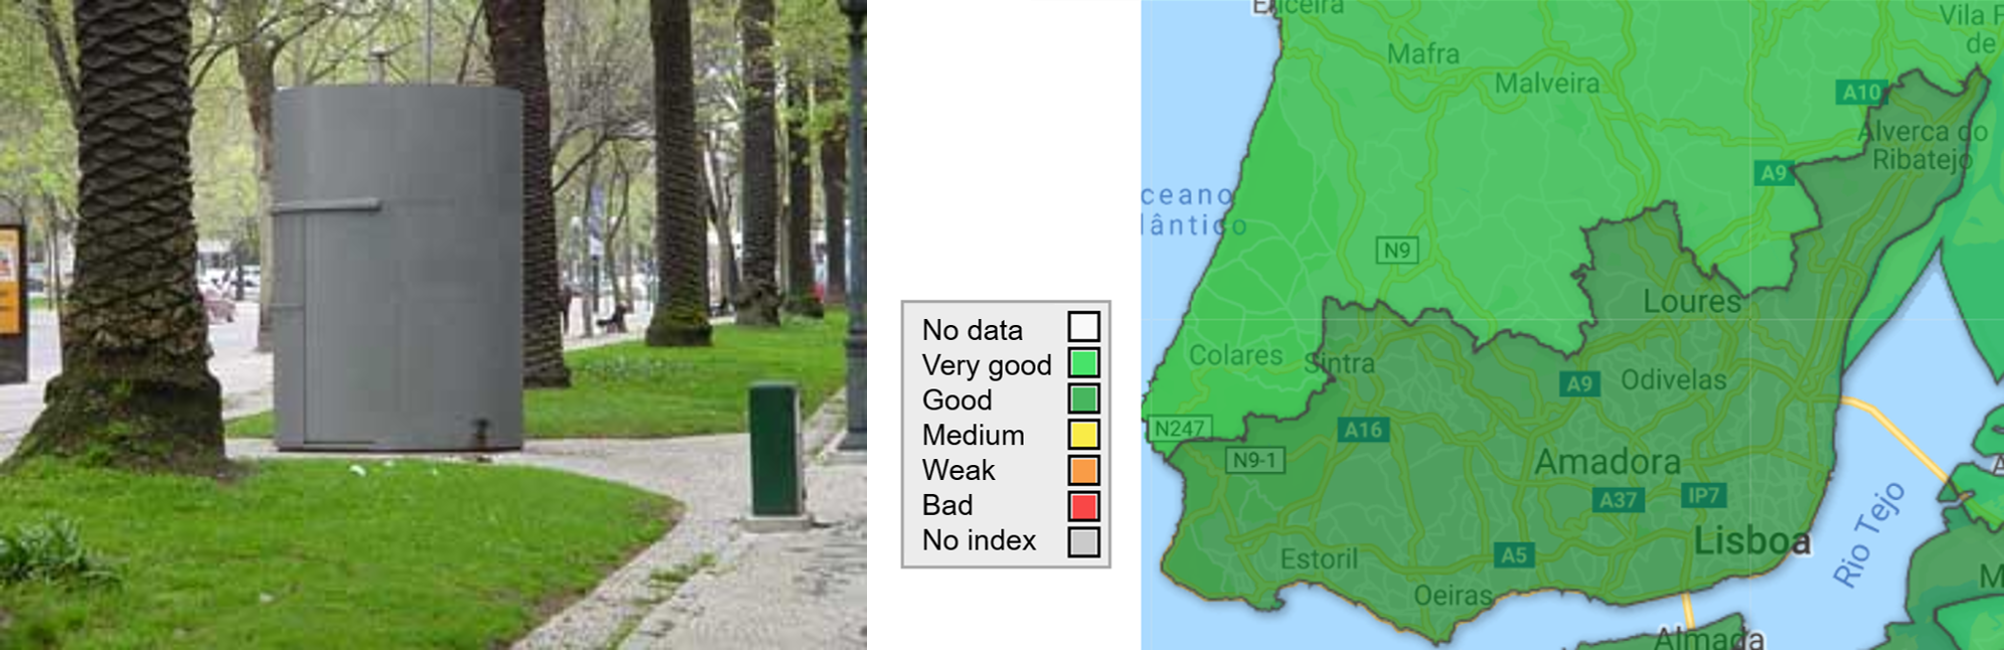
\includegraphics[width=0.9\textwidth]{./Images/ieec1.png}
\caption{Air quality monitoring and information state in Portugal.}
\label{fig:ieec1}
\end{figure}

% #############################################################################
\section{Motivation}


Throughout this and the previous decade, technology has seen big developments in the electronic and telecommunication areas, which has made possible the creation of small and low-cost sensors, compared to the ones in the aforementioned conventional systems. These sensors can be combined with electronics and technologies such as mobile communications and the \ac{IoT} to provide cheaper and more effective solutions to the current systems. With the objective of tackling the low amount of resources to model air pollution with a more granular space-time resolution, some governments are already developing initiatives with the use of these new technologies \cite{GSMA2018}.

Modelling and air quality data processing also play a big role in the control of air pollution, by providing tools for a better visualization of its evolution. This knowledge facilitates urban management, through the attainment of risk maps, which are very useful in critical situations. These provide information that raises the awareness of citizens, to change their lifestyle habits, according to the pollution in their cities, and therefore minimizing their own exposure to air pollution \cite{GSMA2018}.

In this work, from all air polluting substances, higher importance will be given to \ac{PM}, which comprises small, solid particles that are a complex mixture of chemical species, originated by a variety of sources, from anthropogenic, mainly combustion processes, to natural, such as storms, pollen and forest fires. According to \ac{EEA}, in 2017, many European cities have shown concentration values of these particles above the limit values \cite{EEA2018}. These particles can penetrate airways, lungs and blood vessels and are known to be responsible for cardiovascular and respiratory diseases as well as lung cancers. Furthermore, PM2.5 particles include pollutants such as sulfate, nitrates and black carbon, which are carcinogenic and pose the greatest risks to human health \cite{WHO2018}.

\subsection{Objectives}

The goal of this work is to develop a system for an high resolution display of PM10 concentration levels throughout the greater area of Lisbon, with the use of the latest IoT technologies available, spatial interpolation algorithms, machine learning and a web application.

The development of this system will be composed of multiple phases. First, a low-cost portable IoT PM sensing system will be developed. Second, with the help of the Lisbon air quality measures and QualAr data, several \ac{SIM}s will be assessed and compared with \ac{FBN}s in what regards spatial interpolation performance. Finally, a web application which is able to present live, fine resolution, interpolated data on PM10 concentration in the city of Lisbon will be built.

The interpolation algorithms will be evaluated based on the measures taken by the network of monitoring stations in the greater area of Lisbon and which data is available in QualAr. This database comprises validated measurement data from the year 1995 to 2017, depending on the availability of each station of the network at that time.

The development of the aforementioned system aims to tackle the current presentation of data regarding air quality, which at the moment is characterized by its coarse and poor resolution, as can be observed in \Cref{fig:ieec1}.

In \Cref{fig:methodology-flowchart} is presented a flowchart with all the steps that constitute the development of the IoT PM monitoring and presentation system.

% TODO
\begin{figure}[ht]
\centering
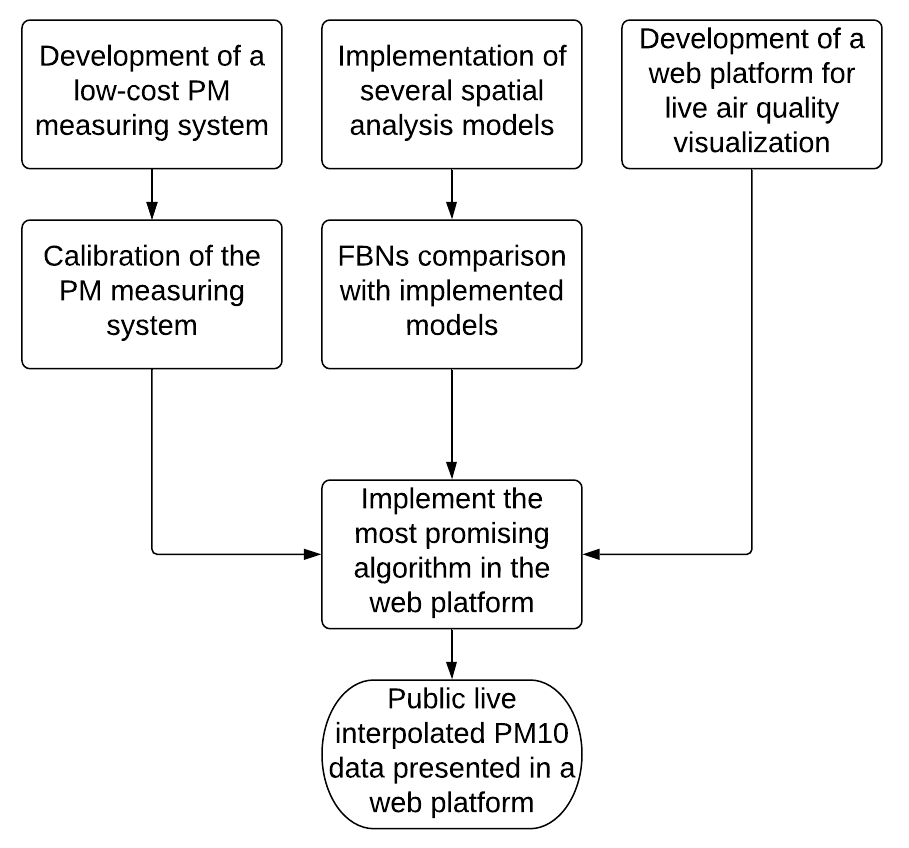
\includegraphics[width=0.64\textwidth]{./Images/methodology-flowchart.png}
\caption{Development of the IoT PM monitoring and presentation system.}
\label{fig:methodology-flowchart}
\end{figure}

% #############################################################################
\section{Claim of Contributions}

This thesis has the following contributions:

\begin{itemize}
  \item The development of an usable, affordable, and portable \ac{NB-IoT} system used for measurement of PM10 and PM2.5. In the future, this could be particularly useful for the integration of these affordable systems in the official air pollution monitoring networks.
  \item An evaluation of FBN interpolation capabilities, as well as a review of state-of-the-art SIMs, in the scope of air quality spatial interpolation applied with the state of information, in the city of Lisbon, available at the time of this thesis.
  \item The development of a web application that is able to present live interpolated PM pollution data in the city of Lisbon, with live data provided by QualAr.
  
\end{itemize}


% #############################################################################
\section{Contents}

\Cref{chap:intro} is the Introduction. It contains an overview over the topic of this work, with air pollution being revealed as a global environmental concern. A description of the motivation, objectives and contributions of this work is provided.

In \Cref{chap:back}, technologies and studies related to the field of work are reviewed, mainly in what regards performance of low-cost sensors, IoT technologies and SIMs. There is also an overview on the current forms of public presentation of available air quality data.

\Cref{chap:architecture} presents every step and methodology that will be used in this work, in detail, from the circuit development and algorithm testing, to the building of the web application prototype.

In \Cref{chap:implement}, the research and development process is concluded with an overview of the results of the built systems and the tested algorithms, along with its discussion and assessment.

In \Cref{chap:conclusion}, the main conclusions attained by this thesis are provided, along with the evaluation of its contributions and the future work that can be developed.
% If Printing on DOUBLE SIDED pages, the second page should be white.
% Otherwise, comment the following command:
\cleardoublepage
%
%Chapter 2
% #############################################################################
% This is Chapter 2
% !TEX root = ../main.tex
% #############################################################################
% Change the Name of the Chapter i the following line
\fancychapter{State of the Art}
\cleardoublepage
% The following line allows to ref this chapter
\label{chap:back}

In this section, a state-of-the-art analysis will be made to the current literature and technologies regarding the main subjects of this thesis. These will encompass the existing projects and sensors for the measurement of air quality, specifically regarding PM, the \ac{LPWAN} IoT technologies and hardware platforms used along with these in remote systems development, the current SIMs and algorithms used for environmental phenomena estimation and visualization, and finally, the current available solutions at public disposal for the visualization of live air quality, in the form of web applications.

% #############################################################################
\section{PM Measurement}

There are many types of instruments and methods for the measurement of the concentration and size distribution of PM. These rely on the various behavior characteristics of particles (mobility, aerodynamics and diffusion) \cite{Amaral2015}. The scope of this thesis only encompasses the measurement of the concentration of PM10 and PM2.5, due to its harm to human health, reviewed in the previous chapter, therefore no size distribution methods will be described. 

The main methods for the measurement of PM concentration in ambient air are gravimetric, optical and microbalance \cite{Amaral2015}.


\subsection{Gravimetric}

The gravimetric method is the European reference method for sampling and determining PM10 and PM2.5 in ambient air, as in the norm EN 12341:2014. 

In the gravimetric method, particle mass concentration is determined through the usage of filters to weigh particles, before and after the sampling period. It is considered as the basic method to measure PM mass concentrations in combustion gases. The filter collects PM in all granulometric fractions and sizes and then a cyclone or impactor is used to remove larger particles. These filters can only output measures from 15 to 15 minutes, therefore this method is not ideal for the identification of real time events. However, the collected particles can be analyzed chemically, which is not possible in some of the other methods.
The filters used in this method are very condition and calibration dependant \cite{Amaral2015}. 

%In Figure XX is presented an example of a reference high-volume gravimetric sensor equipment, Sierra-Andersen


\subsection{Optical}

Optical instruments can be based on the principles of light scattering, absorption or extinction, with scattering being the most usual. They usually include dispersion photometers for the measurement of the intensity of scattered light in one or more angles from a combination of all the particles present in the optical detection volume. 
In the light scattering methods, particles are hit by a light beam and irradiate that light in every direction.
Most commercial light scattering instruments use visible light and measuring angles of 90°, 45°, or less than 30° \cite{Amaral2015}.


\subsection{Microbalance}

In the microbalance method, particles are collected into the surface of an oscillatory microbalance, then through oscillation, these use the alteration of resonance frequency to determine PM concentration.
For this method there are two main prevalent instruments, the Tapered Element Oscillation Microbalance and the Quartz Crystal Microbalance.

In the first one, PM mass is measured based on the alteration of resonance frequency of a tapered quartz wand, according to the accumulation of particles in a sampling filter, connected to the wand. In the second, the quartz crystal has a piezoelectric property of changing its resonance frequency when there is a small addition of mass in its surface, with particles being deposited by electrostatic precipitation in a fine quartz
crystal resonator, instead of a sampling filter \cite{Amaral2015}.

Amaral et al., in 2015, reviewed every type of PM instrument available in the market, with the goal of helping researchers choose the most suitable equipment for their application. It was concluded that when deciding which device is most appropriate, issues such as detection limit and size range of the instrument must be evaluated \cite{Amaral2015}. 

Regarding specific instruments, it was concluded that methods which use filters are not very accurate, but have the advantage of performing chemical analysis in the measured particles. It also requires a lot of labor for it to function properly. Finally, it is also concluded that there was not an absolute best instrument for measuring PM, but a most suitable for each situation, and that different methods should simultaneously be used, in order to confirm values during sampling.


\subsection{Portuguese Monitoring Station Network}

In \Cref{fig:apa-stations-location} is presented the current monitoring network in the county of Lisbon presented in QualAr website, where it is possible to see the available stations at a certain time, along with color graded measures from the available stations \cite{QualAr}.
In Portugal, according to the Manual on Methods and Operational Procedures of Air Quality Monitoring Networks, made by the Portuguese Environmental Reference Laboratory, the methods used for the measurement of PM10 and PM2.5 are the gravimetric and the beta ray absorption \cite{LaboratoriodeReferenciadoAmbiente2010}.

The gravimetric method works as stated in Section 2.1.1. It allows determining the mass of particles deposited in the filters, and these are later used in laboratory to determine particle chemical properties \cite{LaboratoriodeReferenciadoAmbiente2010}.


The monitor used at the stations at the time of this thesis, which was used as reference in this work, was the Environnement S.A. Model MP101M, which is certified equivalent to the reference method in accordance with the EN12341 European standards for PM10 and PM2.5 particulate concentration. It is based on the beta ray attenuation measurement technique, which is an optical light absorption PM concentration measurement method \cite{environnementSA}.

A schematic summary of every PM concentration measurement method analysed in this section is presented in \Cref{fig:pm-measurement-methods}.

\begin{figure}[ht]
\centering
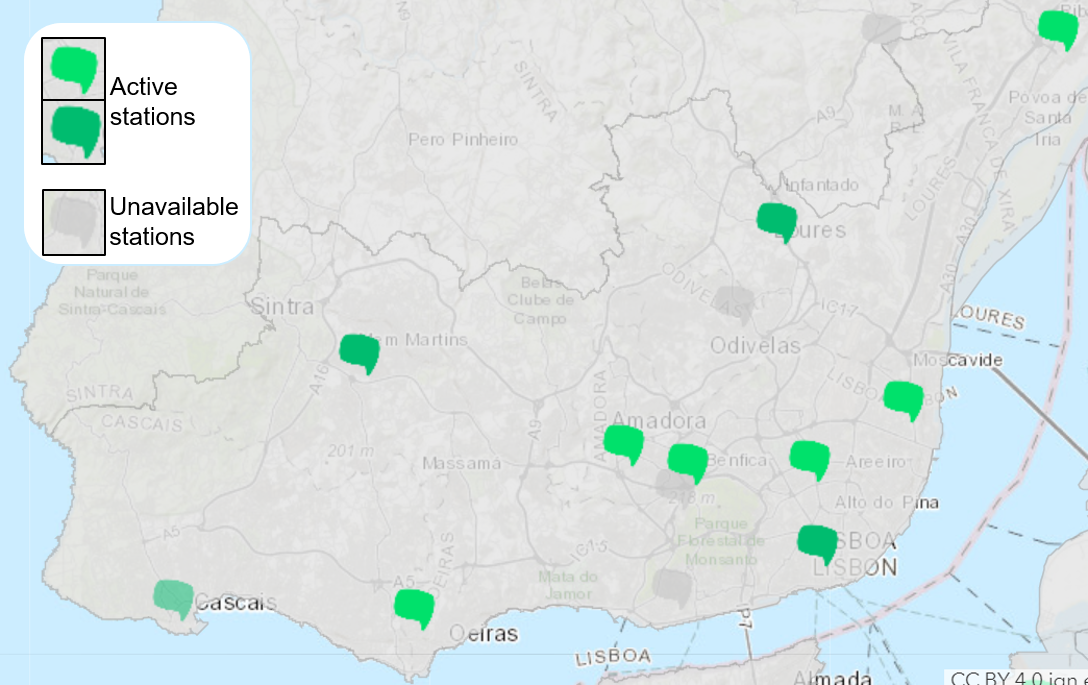
\includegraphics[width=0.8\textwidth]{./Images/apa-stations-location.PNG}
\caption{Current monitoring network in the county of Lisbon.}
\label{fig:apa-stations-location}
\end{figure}

\begin{figure}[ht]
\centering
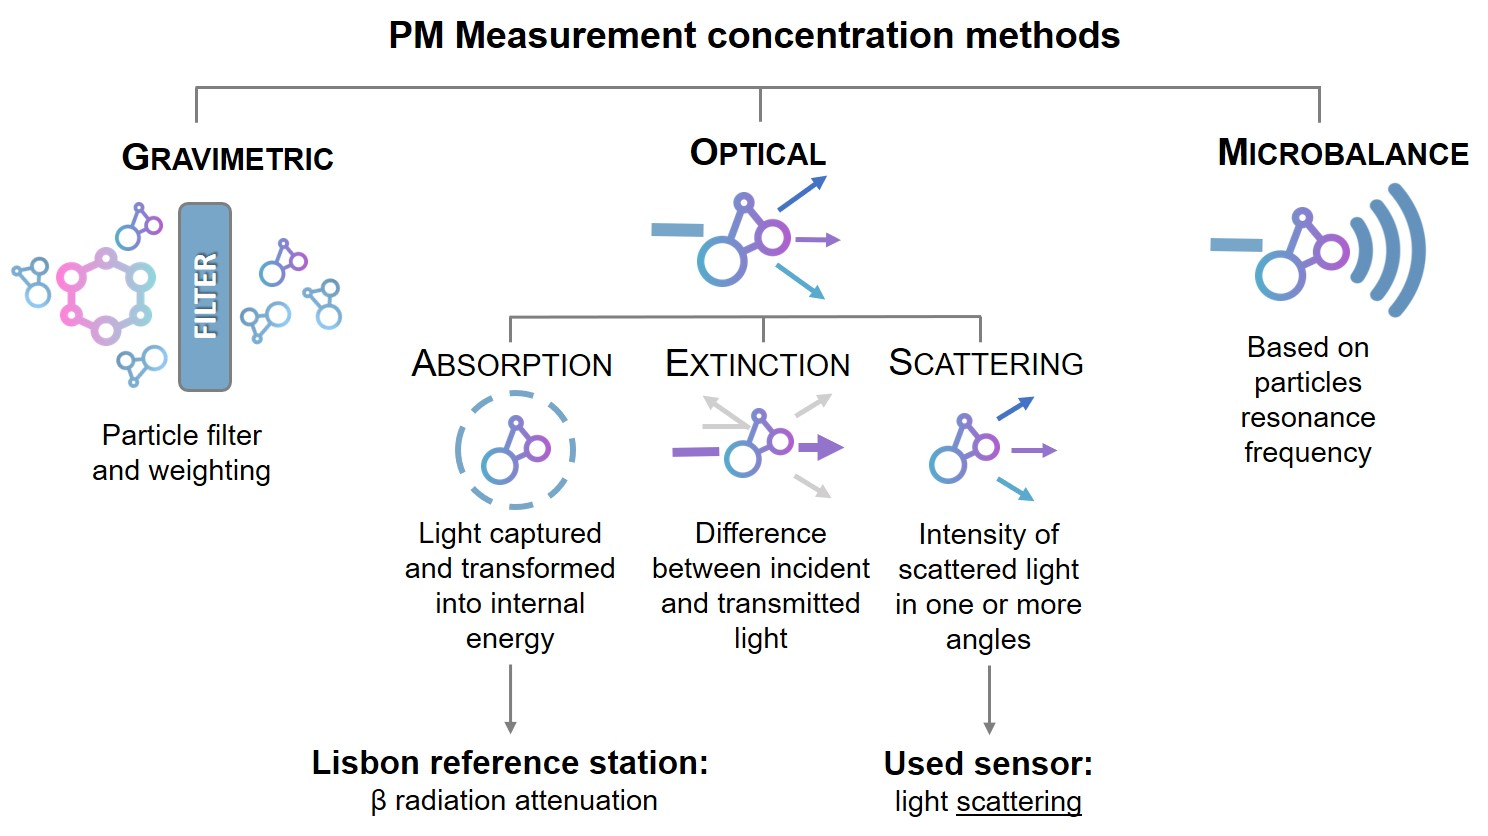
\includegraphics[width=0.9\textwidth]{./Images/pm-measurement-methods.jpg}
\caption{PM concentration measurement methods.}
\label{fig:pm-measurement-methods}
\end{figure}

% #############################################################################
\section{Low-cost Air Monitoring Systems}

The scope of this thesis is aimed at the usage of low-cost sensors to further extend current monitoring networks with more data. For this to work, some examples of usage of low-cost sensors were observed in the literature in order to conclude whether these low-cost PM sensors are reliable, taking into account its performance, cost, and calibration needs.

Several models for monitoring systems have been developed with the objective of providing a better solution for the monitoring of air pollution with much lower maintenance and production costs than the current monitoring stations. Many of these use IoT devices and take advantage from mobile communication technologies \cite{Zheng2018}\cite{Wendt2019}\cite{Quelhas2011}. 

In this section, first there will be an overview over research projects and dissertations prior to this thesis where air quality was attempted to be measured at low-costs. Second, it will be shown literature regarding the performance of low-cost PM sensors currently available in the market.

\subsection{Previous Projects}

In 2008, Carvalho developed, in his thesis, a mobile system to monitor air quality which could be connected to mobile objects such as a bus or a taxi, in order to acquire a map of the quality of air \cite{Carvalho2008}. This system had a \ac{GPS} module to provide the location of the system and a \ac{GSM} module to transmit data to a central server. The measured gases were CO, NO2, O3, SO2 and CO2, therefore PM measures were absent. Each module was self-sufficient and supplied by solar panel charged batteries, and the gases measures were presented in the server in a numerical or geographical form overlapped with a map of the city of Lisbon. However not many campaigns were done, with not much data being collected, and the system's sensors were not calibrated with the reference standard measuring stations. 

In 2011, in the context of an improvement of air quality project named URBISNET, which took place in Lisbon, made by several researchers from Instituto Superior Técnico, a prototype of a mobile station for air quality mapping sensor network was developed \cite{Quelhas2011}. This prototype also measured many polluting gases, used GPS, significant processing power, data storage, many inputs and outputs for the different sensors, and GSM. Despite the efforts on the development of this solution, there were problems with the calibration and overall validation of some of the low-cost gas sensors, which rendered the prototype not very useful and with relatively high production costs for the functions provided.

Vehicle and Propulsion Systems Laboratory, currently operating in Instituto Superior Técnico, in its proposal of creation, with the coordination of Tiago Farias, proposed a project for monitoring pedestrians exposure to PM \cite{Farias2013}. This consisted of a 11 kg bag, with a GPS module, a micro-controller, a particulate and dust sensor, a numerical pad and a computer. The collection of particle concentration data combined with nearly instant measures and the live GPS monitoring allow the estimation of the pollution pedestrians are exposed to throughout certain routes.

\subsection{Low-cost PM sensors}

Low-cost solutions for PM measurement currently in the market consist mostly of optical instruments. These are made of small lasers placed in an certain angle, against a photodiode, which is used to detect the scattered light of illuminated particles, as stated in Section 2.1.2. The generated light scattering signal is filtered and amplified. Afterwards a modulation signal is used to represent the measurements. These sensors usually cost less than 50 euros, which is a considerable difference in relation to reference instruments, which have much more expensive production and maintenance costs.

Despite their price, low-cost optical PM monitors can be used to characterize PM concentrations with high spatial and temporal resolution \cite{Manikonda2016}. In 2016, Manikonda et al. conducted a study with the objective of assessing these monitors and concluded that they perform with adequate precision for indoor air monitoring, although with some calibration requirements \cite{Manikonda2016}. Currently, many professional small factor air quality monitoring stations, for both indoor and outdoor applications, are available in the market. Additionally, communities have been formed with the objective of creating networks where individuals can collect and share data from their personal monitoring systems so that all the obtained data is presented collectively in a map. An example of this is the Weather Underground community \cite{WeatherUnderg2019}.

Some of these monitoring stations are known to use low-cost and compact size light-scattering based PM sensors, namely, the stations manufactured by Gaia Earth Sensing Labs, which use specifically Plantower PMS sensors \cite{AQICN}. These manufacturers have many product variants for outdoor monitoring. One of these products is presented in \Cref{fig:ieec3}.

\begin{figure}[ht]
\centering
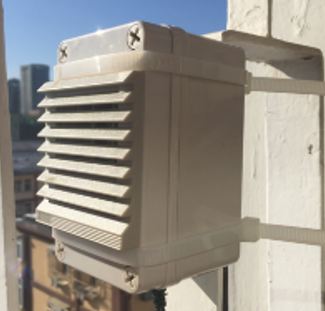
\includegraphics[width=0.4\textwidth]{./Images/ieec3.png}
\caption{Example of commercialized PM monitors.}
\label{fig:ieec3}
\end{figure}

A study from the University of Utah, in 2018, performed a long-term field evaluation of the Plantower PMS sensors, in which for 320 days, multiple season variations, and significant PM2.5 variation events, measurements were undertaken by two sensors, PMS5003 and two PMS1003, with tracking made through co-located reference air monitors. The results of this study demonstrated overall good correlations between the PMS sensors and reference monitors in the winter season, seasonal differences in sensor performance, some intra-sensor variability, and drift in one sensor, with worse results associated to the PMS1003 sensor \cite{Sayahi2018}.


Kuula et al., in 2019, investigated how sensors can be used in urban areas to complement existing air quality networks, through a campaign during the winter, with the use of the optical sensors PPD60PV and PPD42NS. These were also compared to reference instruments \cite{Kuula2019}. The results showed that these sensors could measure PM10 and PM2.5 with reasonably high correlations. It was concluded that comprehensive understanding of the sensor characteristics is necessary, and that the sensor must be validated and calibrated in the environment where it will be placed. It is also stated that one big disadvantage of these sensors is the non-guaranteed accuracy and the lack of established scientific literature. Results also show that optical sensors are suitable for measuring mass concentrations of particles that are larger than 0.5 $µm$, and that diffusion charging based sensors, instruments which use light extinction to monitor particle concentrations, are better for traffic exhaust and local combustion related ultra fine particles.

Despite being promising, the performance of these low-cost PM sensors under field conditions is still not well understood. In order to characterize the performance capabilities of a low-cost PM sensor, PMS3003 from Plantower, Zheng et al., in 2018, performed a study where these sensors were tested in both low and high particle concentration regions, during different seasons, to determine how the sensors perform across a range of concentrations and meteorological factors \cite{Zheng2018}. The attained results showed that \ac{RH} has a major influence in the sensor measures, while the temperature effects were negligible. With that, calibration correction factors were applied to measures taken by the sensor, and the mean errors were reduced from 27\% to 10\% at different time resolutions, when compared to high precision reference instruments. After calibration, the results proved that the sensor can be a promising addition to current PM sensor networks.

The South Coast Air Quality Management District, agency responsible for South California air quality monitoring, in 2018, field-tested Plantower PMS5003 PM sensor, and notable correlation and precision was attained between the PMS5003 and the reference instruments \cite{AQ-SPEC}.


% #############################################################################
\section{Interpolation Algorithms for Spatial Analysis}

Air quality analysis relies in mathematical approaches to explain the polluting gases concentration evolution. The process of developing this type of prevision with high spatial resolution is a rather complex problem, due to the wide sources of pollution in urban and industrial areas, and to all the variables that can influence air quality.

Approaches to this problem in the literature are sometimes deterministic, which require a lot of knowledge on the local sources and factors that can influence air pollution, or otherwise rely on measurement data. Spatial interpolation consists in estimating the value of measures of certain properties, at unsampled locations, within the area covered by existing observations of the same properties. The objective is to present a much more detailed overview of the air quality in a certain region.

Currently, SIMs are well developed and frequently used in various \ac{GIS} applications, in which they can be used to manipulate, analyze and present data in spatial representations. Spatial interpolation is based on the fact that observation points that are closer to each other have more similarities than the ones far away, which is known as Tobler’s First Law of Geography \cite{Stein1994}.

Some of the most popular and standardized SIMs, since the beginning of spatial interpolation modeling, are \ac{IDW}, kriging, shape functions, spline, and trend surface. These occur from different approaches to this problem, such as local neighborhood, geostatistical and variational \cite{Li2008}.

In 2014, Li and Heap made a review of the 25 most commonly applied SIMs \cite{Li2014}. As result an easy to use decision tree was created for use case dependent method selection. According to it, the most suitable interpolation algorithms in circumstances such as the ones in this work are IDW and \ac{OK}, depending on data selection and availability.

\subsection{Fuzzy Boolean Networks}

FBNs are boolean networks developed and studied by researchers at Instituto Superior Técnico \cite{Tome}. 
In order to correctly explain the functioning of these, a proper nomenclature needs to be given to its constituents.

The networks are constituted by neuronal areas. Each area has a set of neurons, and the number of neurons, which is user defined, must be equal in all areas. Each neuron has a binary value and is constituted by a binary table with a user defined length. The value at each index of each table is considered a memory of the respective neuron, and all memories are initialized with a random number between zero and one. The number of memories of each consequent neuron is equal to a granularity factor.

Each neuronal area can only be one of two types, antecedent or consequent, with their corresponding neurons named after the area, antecedent or consequent neurons respectively. FBNs must have at least one neuronal area of each of the two types. In these networks, connections are weightless, temporary, circumstance dependent and only appear between neurons located in different areas of different types, either in the learning or in the inference process.
In \Cref{fig:fbn-drawing} a very simple example of an FBN is presented, with  two antecedent areas and one consequent area, each with four neurons. The granularity factor is two and consequently, neurons in the consequent area have four memories each. In this representation dark neurons have the value one, and white neurons have the value zero.

\begin{figure}[ht]
\centering
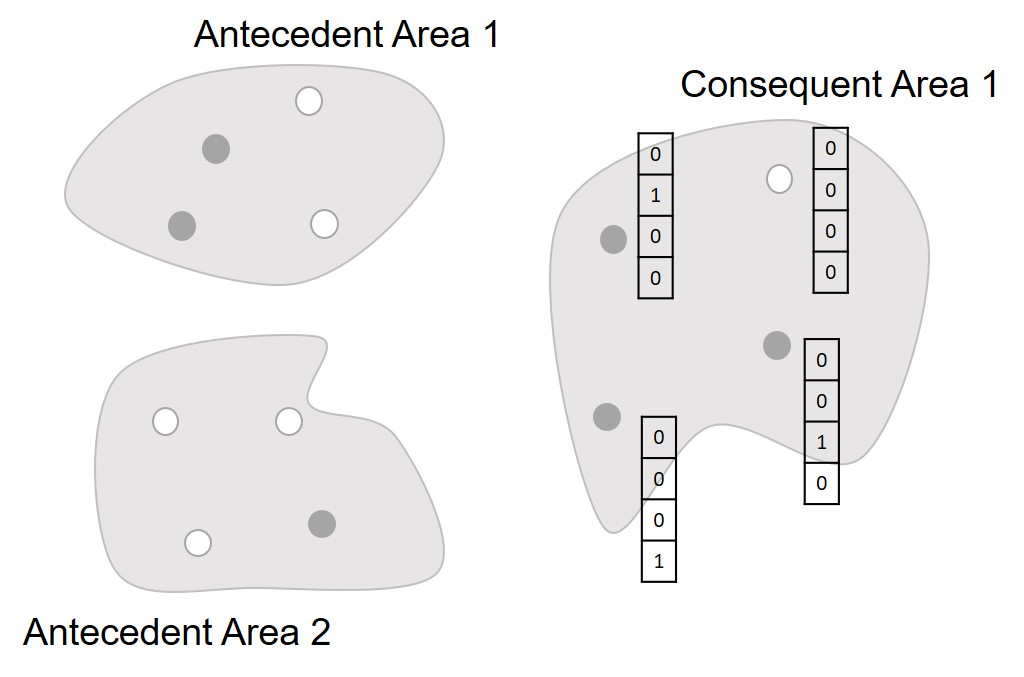
\includegraphics[width=0.65\textwidth]{./Images/fbn-drawing.jpg}
\caption{Example of the constituents of a FBN.}
\label{fig:fbn-drawing}
\end{figure}

In what regards the usage of these networks, the number of areas is defined by the number of variables in the problem. To each independent variable, an antecedent area is created and associated. The same happens with the dependent variables, for which consequent areas are created and respectively associated. As an example of usage, if used for linear interpolation, the FBN would only have an antecedent area, associated to the x axis (independent), and a consequent area, associated to the y axis (dependent). The network represented in \Cref{fig:fbn-drawing} has two independent and one dependent areas, being the latter the subject of inference.

Before the creation of the network, the definition of its parameters must be made. These parameters are the size of each neuronal area, the number of memories per neuron, the granularity factor and the number of samples each neuron uses in the inferring and learning processes. Each should be previously tested and assessed comparatively by the researcher, to each different use case \cite{Tome2014}.

The learning process of these networks is composed of several phases:
\begin{itemize}
\item First, for each network there will be sets of values of each variable in the problem. These are considered the rules that the network will learn. For each set, and for each variable, its value is translated into a percentage. Each corresponding area will be activated according to this percentage, that is, the neuron values for that area will be 1 with the probability of that percentage, and rest will remain at zero.
\item Second, each neuron, in the consequent areas, samples an user defined number of neurons from each antecedent area. This number must always be the same for every neuron and antecedent area, and counts the number of one valued neurons for each area. 
\item For each count that neuron attained, it multiplies that count by the granularity factor raised to the power of the number of the antecedent area of the respective count.
\item Finally, each consequent neuron stores its own binary value (which was defined during the consequent area initial activation) in its memory table, in the index corresponding to the previously acquired count.
\end{itemize}

Various iterations of this process, for different training values for every variable,  represent how training is performed in FBNs.
Assuming each memory was initialized with the value zero, it is possible that the represented FBN has already been trained with exactly one set of values, since one memory per activated consequent neuron has the value of one. In this single learning process step, one could conjecture that the connections for that step were as portrayed in \Cref{fig:fbn-drawing-2}, according to the activated indexes of the table of memories of each consequent neuron (connections with the zero valued neuron in the consequent area were not placed in the figure for ease of visualization, since they are not relevant).

\begin{figure}[ht]
\centering
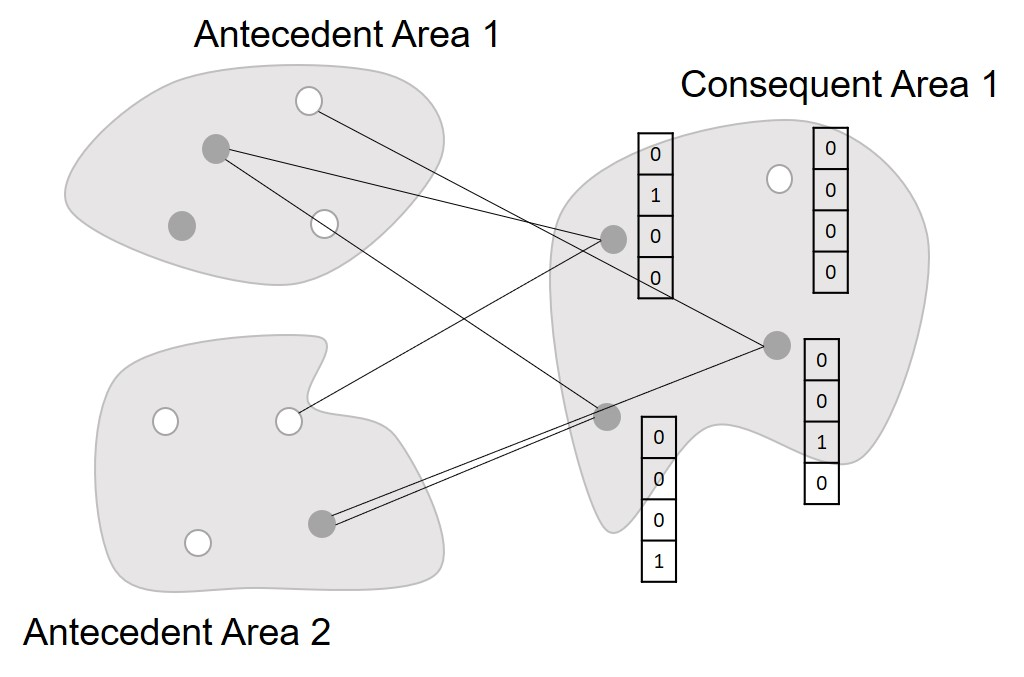
\includegraphics[width=0.65\textwidth]{./Images/fbn-drawing-2.jpg}
\caption{Example of the learning process of a FBN.}
\label{fig:fbn-drawing-2}
\end{figure}

In the inference process, the network only receives the value of the independent variables and it is supposed to infer the dependent variables value:
\begin{itemize}
\item Initially, only the antecedent areas are activated according to its variables value translated into percentage. 
\item Afterwards, in the exact same fashion of the learning process, every consequent neuron performs sampling, ending up with a count for each antecedent area. The value in the corresponding memory of that neuron is verified. If it stores a zero, then that neuron value will be modified to zero, if it stores a one, its value will be modified to one.
\item In the end of this process every neuron in every consequent area will have a binary value. Therefore, consequent areas can be translated into a percentage according to its activation ratio. 
\item This percentage is translated into the scale of the corresponding dependent variable, and it represents the inference value for the respective variable, in the respective set, according to the respective learning rules.
\end{itemize}

Studies have concluded that these networks have many nature and biologic like characteristics, such as the organization of neurons per area, to which a given variable or concept can be associated. They have random individual connections and structured meshes of links between them. They are also characterized by relative noise immunity and the capability to approximate reasoning and learning. Provided the remaining neurons are enough to define activation ratios accurately, any number of neurons or connections may be deleted or corrupted \cite{Tome2014}.

It has also been shown that the FBN learning process converges for a repetitive sequence of different rules, where in the limit, the system is able to learn a number of rules compatible with a granularity that increases with the square root of the number of inputs per neuron and per antecedent \cite{Carvalho2002}.

As Universal Approximators, FBN can learn multi-input single-output functions, and they perform pretty well in comparison to other techniques when parametrization is rather difficult. FBN perform better when the training data is very sparse, and data-sets are imbalanced \cite{Carvalho2007}. They are shown to be immune to individual neuron or connection errors, which does not happen with \ac{ANN}, and also have good generalization capabilities \cite{Carvalho2007}.
However, one problem that arises from the use of FBN is the that the memory necessity increases exponentially with the number of inputs and size of the network, which is a notable limiting factor.

Tomé et al., in 2014, in a deep analysis of FBN, despite assessing its main characteristics and advantages, also made experiments in which learning, and interpolation capabilities were compared, by interpolating sparse data. The comparisons were made between FBN, \ac{ANFIS}, ANN, Cubic spline interpolation, Support Vector Machines and Isotonic Regression Model, and it was shown that FBN outperformed all other interpolation algorithms. Even when used as a classifier, FBN outperformed every other algorithm, given a sparse set of data \cite{Tome2014}.

\subsection{Inverse Distance Weighting}

IDW is a deterministic SIM based on the assumption that the degree of influence of the nearby sample points should be greater than the effect of more distant points. Its maximum and minimum value can not occur outside the sampled points. The only parameter which is user defined in the IDW implementation is the power function, which defines the relevance of the distance to the weights of each observed value \cite{Mesquita2009}.

The IDW interpolation can be defined by the equation \eqref{idw}, where \eqref{idw-weight} represents the weights associated to each observation.

\begin{equation} 
\label{idw}
\scalebox{1.4}{ $ f(x, y) = \dfrac{\sum_{i=1}^{n} w(d_i)z_i}{\sum_{i=1}^{n} w(d_i)}, i = 1, 2, ..., n$}
\end{equation}

\begin{equation} 
\label{idw-weight}
\scalebox{1.3}{ $w(d_i)= \dfrac{1}{{d_i}^{p}}$}
\end{equation}

Where $z_i$ is the observed value, $d_i$ is the distance between the estimation and the observation points, $w(d_i)$ represents the weight associated to observation \textit{i}, and \textit{p} is the power function.

In IDW, weights are proportional to the inverse of the distance elevated to the power of p. Therefore, as distance increases, weights decrease, in a rate that increases the higher the value of p.
When p is zero, the resulting estimate is simply equal to the spatial average of all sampled points.
%The IDW can be either global or local and exact or gradual.

Even though IDW is one of the most widely used interpolation models, it has several limitations, such as its inability to produce error statistics, unlike OK, and the fact that spatial relationships between two locations are not only dependent on distance neither are they constant over space \cite{Mesquita2009}.

\subsection{Kriging}

Kriging interpolation models are fundamental geostatistic tools in the field of spatial analysis.

The main difference between kriging and other non-geostatistical models is the assumption that the spatial correlation structure of the process under study is known and can be estimated from the observed data. In kriging, weights are based not only in the distance between points but also in the overall spatial arrangement of observation points \cite{Mesquita2009}.

The kriging schemes are stochastic, local, gradual and exact interpolators. Its methodology includes two stages: the analysis of the spatial variation and the estimation of the target variable, which is also based on the weighted average approach. Furthermore, it uses several statistic models which allow the construction of a variety of maps, including previsions, errors of previsions and probabilities, which are considerable advantages in comparison to IDW.

Before kriging is used, an exploratory statistical analysis of data must be made, as well as the modelling of a variogram to represent how semivariance varies with distance. The analysis of the spatial variation is performed through the variogram modelling of how distance variations with semivariance are not linear, but have a custom relation. In \Cref{fig:variogram}, an example of a variogram is presented. The nugget represents the semivariance value when the distance tends to zero. The sill is the point where semivariance stabilizes, and range is the interval in which as distance increases, higher is the semivariance. Kriging interpolation weights are chosen using the modeled variogram, so that estimates are unbiased and the estimation variance is minimized.

The most common kriging models are simple kriging, which assumes a known constant mean, OK, which assumes that there is an unknown constant mean, estimated from the data and universal kriging, which assumes that there is a trend in the surface that partly explains the data variations \cite{Deligiorgi2011}.

\begin{figure}[ht]
\centering
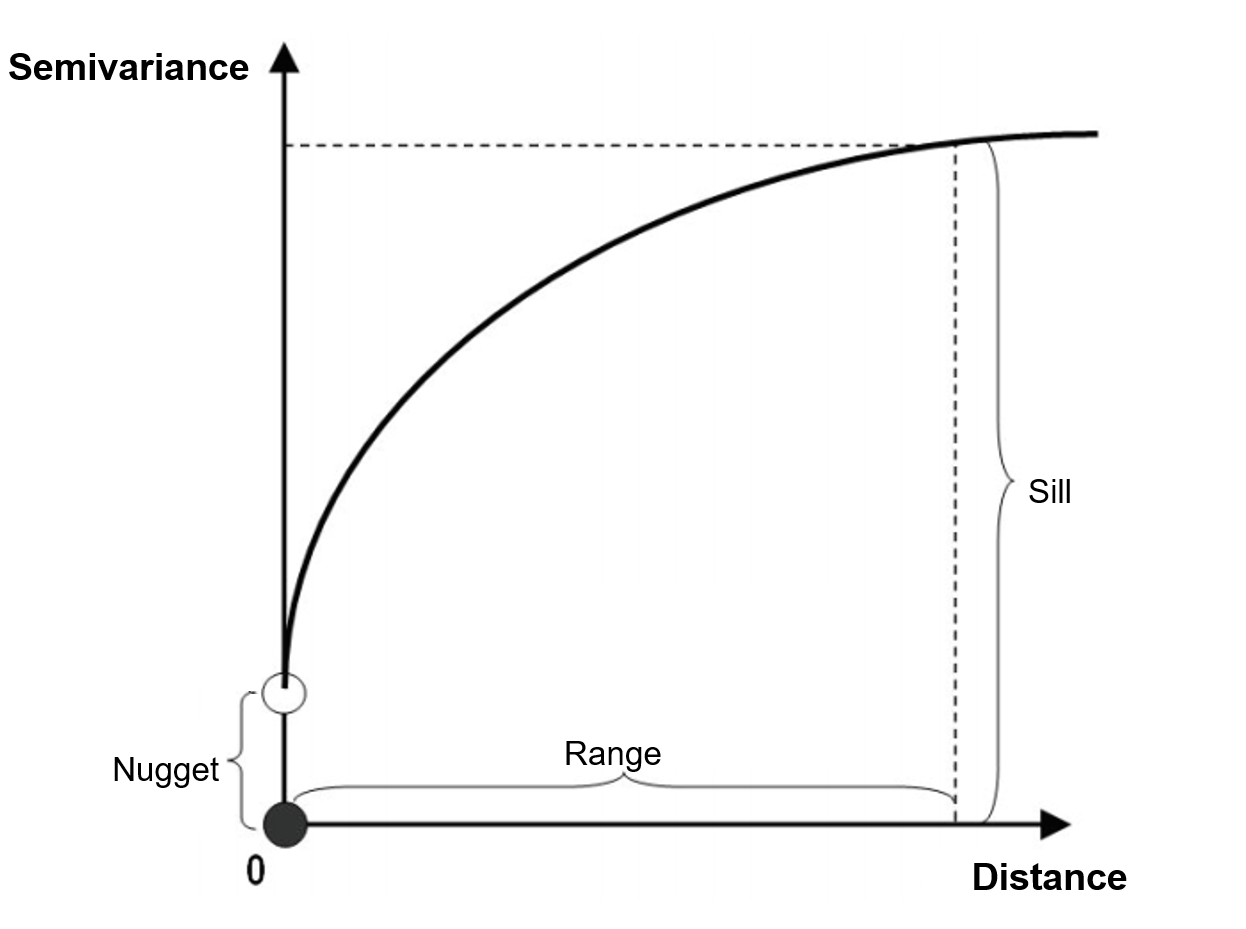
\includegraphics[width=0.6\textwidth]{./Images/variogram.png}
\caption{Example of a kriging variogram.}
\label{fig:variogram}
\end{figure}

\subsection{External Influences}

AERMOD and ADMS-urban are air pollution dispersion models that are reference standards for governments such as the ones of United States of America and United Kingdom for the precision modelling of air quality \cite{Mohan2011}.
AERMOD was developed at the United States Environmental Protection Agency and ADMS-Urban was developed by Cambridge Environmental Research Consultants. Both are used for regulatory purposes in the respective countries and highly recommended models in many other.

AERMOD is a gaussian plume air dispersion model which heavily takes meteorological and other external factors into account. The fact that it is plume based model, means that it considers the movement of one fluid through another, which in this case are the particles which move through the air. Some of the external factors which it takes into account are cloud cover observations, wind speed and direction, temperature, dew point,
humidity and sea level pressure. Meteorological data is accepted from multiple heights and wind, temperature and turbulence are treated as vertical profiles.

ADMS-Urban is a model of dispersion of pollutants released from industrial, domestic and road traffic sources in urban areas. This local Gaussian type model is nested within a trajectory model for areas within 50 km × 50 km \cite{Lee2013}.

These models recognize that air turbulence and dispersion are continuously variable, depending on height above ground, winds and temperature. Concerning the height above ground, virtually all airflow near the ground is neutral. Both models have steady state by nature, which means polluting gases conditions, between the time of emission and the time it reaches any receptor, do not change. Therefore, it is clear that plume models cannot be expected to give reasonable results for long range transport of pollutants.
Despite this, they can still be used to estimate pollutants concentration in areas where there is no monitoring stations, in the likes of interpolation methods \cite{Lee2013}.

In 2009, Mesquita, studied the performance of Multiple Linear Regression as an interpolation algorithm that uses external factors like city traffic emissions in comparison to the most common interpolation algorithms which do not encompass external factors, and this approach reflected notably better results than algorithms such as IDW and OK \cite{Mesquita2009}.


\subsection{Temporal Forecasting}

Zhang et al., in 2012, made a complete two part review of the history, techniques, current status of science and research and future prospects of real time air quality forecasting, where three major techniques for forecasting are distinguished \cite{Zhang2012} \cite{Zhang2012a}.

The simple empirical approaches, which are based on the assumption that today’s observed pollutant level is tomorrow’s forecasted value, are considered weak and of low accuracy. There are also parametric and statistical methods, which encompass regression methods and ANNs, and provide moderate to high accuracy. Finally, there are the advanced, physics based approaches, which are computationally expensive and complex and have very high operational costs and also have moderate to high accuracy \cite{Zhang2012}.

It is important to notice that for real time air quality forecasting, most methods are very circumstance dependent and regional related, with a big knowledge needed on the area subject to the forecasts.

Real time air quality forecasting does not belong to the scope of air spatial interpolation, therefore it will not be subject of study in this thesis but it could be considered for a prospect of future work for the developed systems.


\subsection{Practical Applications}

The above mentioned approaches have been developed and experimented both theoretically and empirically, with many of its applications documented in recent literature in the air pollution field.

A review of SIMs for environmental scientists made in 2008, by Li and Heap, theoretically compares 26 SIMs and concludes that the selection of an appropriate method for each different case is critical, but difficult, since its performance depends on the variable under study, the spatial configuration of the data and on the underlying assumptions \cite{Li2008}.

In 2013, Funenga, in his masters dissertation, used the OK interpolation method to infer the air quality related to polluting gases in the city of Lisbon, with the data available from the fixed monitoring stations \cite{Funenga2013}. The results showed poorly defined spatial continuity, since the interpolation only accepted inputs from 6 different stations, which represent very sparse data. Funenga also tested the Calpuff model for interpolation, which was, until 2017, the preferred system for the simulation of air pollution dispersion of the United States Environmental Protection Agency. This consisted of a model for the meteorological factors influence, a Gaussian puff dispersion model and a post-processing program for results output. In comparison to the OK, this model relative mean absolute error was lowered, which demonstrates high performance increase from the Calpuff method usage.

Tang et al., in 2017, proposed a spatial interpolation framework to incorporate diverse data sources and model the spatial processes explicitly at multiple resolutions with the use of spectral analysis and a spatial Gaussian process for interpolation, underlining the fact that when monitoring data sources are very sparse, auxiliary data should be added to the interpolation algorithms \cite{Tang2017}.

In 2018, Oteros et al., based on weather information, and on a kriging geospatial interpolation method, estimated daily pollen concentration in unmonitored areas, based on 26 monitoring stations in an area of approximately 71 000 km$^{2}$. It concluded, that the developed system was accurate enough for the spatial interpolation of pollen concentrations at unmonitored sites \cite{Oteros2018}.
Also in 2018, a study was conducted with the objective of proposing a low-cost mobile sensor network for evaluation of air quality in urban areas, with the use of kriging interpolation for data processing. It concluded that better results could have been taken if the modelling relied not only on measurements but also on spatial information such as weather data, building heights, and population density. It also confirmed that sparsely distributed sensor nodes, along with kriging interpolation, can be used to produce a real-time rendering air quality map \cite{Makowski}.

Machine learning techniques have also been incorporated into air quality interpolation, in order to improve its results and some of its processing and data constraints. 

Mishra et al., in 2015, used an artificial intelligence approach to forecast PM2.5 during haze episodes, compared Neuro-Fuzzy techniques with ANNs and Multiple Linear Regression, and concluded that its Neuro-Fuzzy model outperformed all the other approaches in the forecasting of PM2.5 \cite{Mishra2015}.

In 2018, Alimissis et al., evaluated both ANN and Multiple Linear Regression as interpolation methodologies, using data from a real urban air quality monitoring network of the concentration of different air pollutants in Athens, Greece. It was concluded that ANN were significantly better, especially where the monitoring network density was limited and there was consequently a low degree of correlation between the monitoring sites \cite{Alimissis2018}. Also in 2018, Franceschi et al. developed models to forecast particulate matter concentration using ANN, which were proven to be useful as references to issue early warnings of high air pollution in certain areas \cite{Franceschi2018}.

Measurement sensors are typically sparsely located, and that is one of the biggest problems to SIMs for the prediction of air pollution.

%In \Cref{fig:spatial-algorithms} are presented the models for %spatial air quality analysis, which are considered in this %work and will be tested in terms of overall performance for %an implementation as a live web visualization of the \ac{PM} %pollution in the city of Lisbon.

%\begin{figure}[h]
%\centering
%\includegraphics[width=1\textwidth]{./Images/spatial-algorithm%s.png}
%\caption{\ac{SIM}s considered in this work.}
%\label{fig:spatial-algorithms}
%\end{figure}

% #############################################################################
\section{LPWAN Technologies}

Small devices with \ac{CPU}, memory, sensors and capable of mobile communications through which they can connect to the internet have a great potential to change our society. The inter-networking of these devices is called IoT. Data collected can be shared and analyzed in real time through the Internet. These objects and networks can help improve society and its citizens lives in many different ways.

In fact, the number of devices connected to the Internet has seen a big growth in the recent years and is expected to keep growing exponentially, as people increase the devices they purchase. This growth is unprecedented in the communication industry as well as in the wider global economy. It is estimated that by 2020, more than 50 billion devices will be connected through radio communications \cite{Holler2014}.

IoT has seen various applications in many practical research fields, due to specific requirements such as long range, low data rate, low energy consumption and cost effectiveness.

The most widely used radio technologies nowadays are either short-range technologies such as Zigbee, Bluetooth and Wi-Fi (which are not suited for scenarios that require long-range transmission), or cellular communication technologies, such as 2G, 3G and 4G (which provide long-range access but have excessive power consumption) \cite{Mekki2018}. With this gap in the radio communications and the emerging IoT technologies, increasing number of devices and many useful practical application projections, a new group of technologies was developed so that long-range transmission could be provided with low consumption and communication costs, named LPWAN \cite{Mekki2018}. This group of technologies is considered to be ideal for the research to be developed in this work, with its application to the system that will be produced. It can be used since a low data rate is allowed, and long-range access together with low-consumption are needed.

LPWAN represents the current trend in the evolution of IoT technologies as it is increasingly gaining popularity both in industrial and research environments, due to its low production and consumption costs. In order to achieve these specifications, usually a small data rate limitation is imposed. LPWAN technologies are an excellent choice for long-term monitoring applications in urban areas, as can be seen by its advantages in \Cref{fig:ieec4}.

Until the appearance of LPWAN technologies, the two main approaches to IoT were multi-hop mesh networks with short-range technologies in the unlicensed spectrum or long-range conventional cellular technologies such as GSM and \ac{GPRS} \cite{Zanella2016}. Experimental trials made by Zanella et al. in 2016 allowed the conclusion that by using LPWAN technologies, less than half of the gateways are needed to cover the same urban area than the number of sites deployed by one of the major cellular operators in Italy, to provide mobile cellular access.

Currently, there are several LPWAN technologies being used both for research and business applications. The most popular and suitable for this work are SigFox, \ac{LoRaWAN}, \ac{LTE-M} and NB-IoT. While SigFox and LoRaWAN are proprietary technologies, operating in the unlicensed spectrum, LTE-M and NB-IoT are standardized by \ac{3GPP} and operate in the licensed spectrum. In this section, an overview of these technologies is made, as well as a comparative analysis regarding related empiric studies in the literature and the characteristics that differentiate them from each other.

The business and commercialization application of LPWAN is already taking place. A survey on LPWAN technologies, made in 2017, stated that the successful implementation of LPWAN technologies such as NB-IoT and LoRaWAN had already been started in North America and Europe. Meanwhile, several mobile operators in countries like Korea, Japan and China, according to the survey, also already had plans to implement nationwide NB-IoT or LoRaWAN \cite{Sinha2017}. 

In Portugal, the mobile operator Altice Portugal has announced total NB-IoT coverage in Portugal by the beginning of 2019 \cite{Altice2018}. 

The rest of the LPWAN technologies have the following coverage in Portugal, at the time of this thesis: SigFox has full coverage, according to its website \cite{SigFox2018}; LoRaWAN has decent coverage, available through a total of 43 gateways implemented throughout the country by several communities in Portugal \cite{ThingsNetwork2019}; there is currently no record of any LTE-M implementation. 

\begin{figure}[ht]
\centering
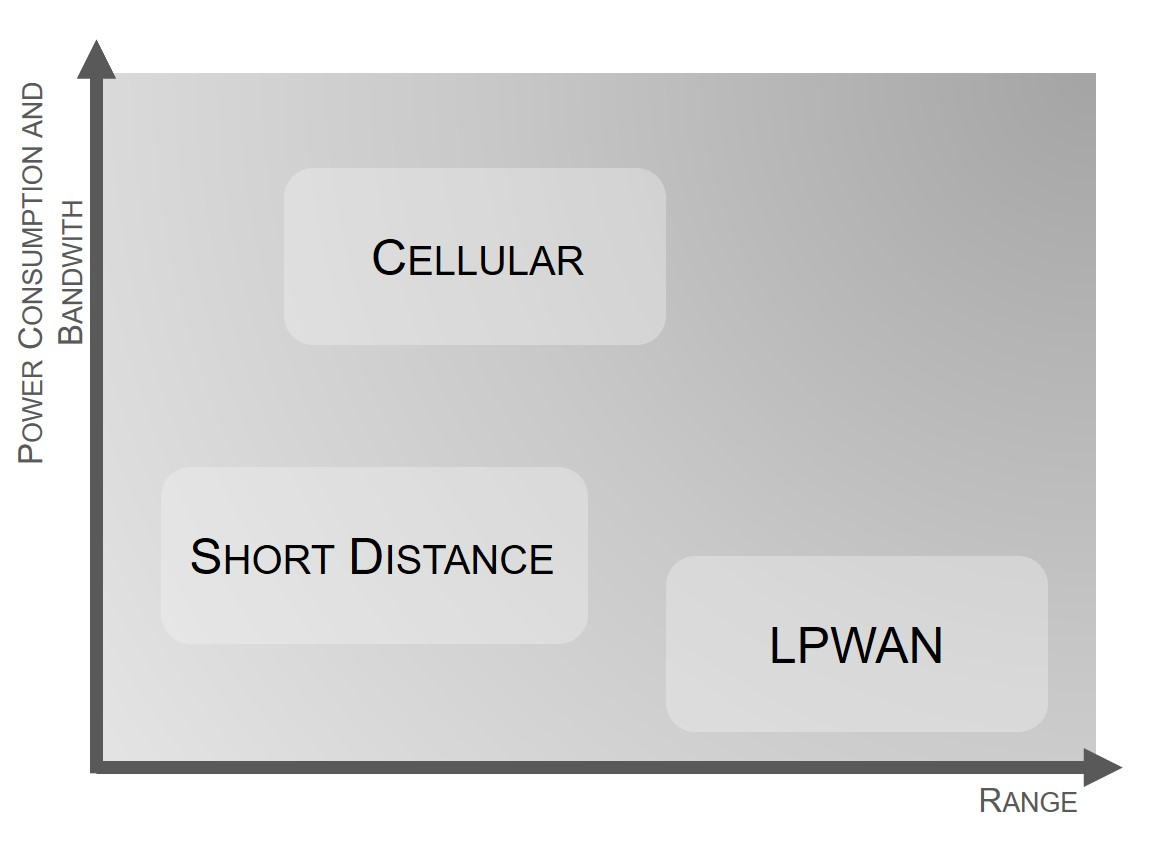
\includegraphics[width=0.6\textwidth]{./Images/ieec4.jpg}
\caption{Comparison of LPWAN with other technologies.}
\label{fig:ieec4}
\end{figure}

\subsection{SigFox}

The SigFox physical layer employs \ac{UNB} wireless modulation, and its network layer protocols are proprietary. Bidirectional communication is supported and SigFox claims that each gateway can handle up to a million connected objects, with a coverage area of 30 to 50 km in rural areas and 3 to 10 km in urban areas.

The ultra-narrow-band technology has communication channels with approximate bandwidth of 100Hz, uplink-triggered transmissions that follow a client-server model and cooperative reception from multiple gateways. An end device wakes up only when uplink data arrives, and then randomly selects a channel for uplink transmission, which is repeated three times to increase the chances of a successful reception by the network. Following this uplink transmission, for the next 10s, there is the possibility for receiving a downlink message on a predetermined channel \cite{Yang2017}.

\subsection{LoRaWAN}

LoRaWAN is another popular LPWAN solution, patented by Semtech Corporation. It has a proprietary \ac{PHY}, \ac{LoRa}, but the rest of the protocol stack, designated LoRaWAN, is open. LoRaWAN networks, like SigFox, typically have a star topology with many end devices connected by a single-hop link to gateways, which are connected to a common network server via standard IP protocols, with its gateways
being totally transparent to end devices, providing simpler network management.

LoRaWAN supports 3 types of end devices, each type characterized as a class. Class A supports bidirectional communications through, right after uplink transmission, two short period downlink receive windows. This class has the lowest power consumption, but like SigFox, for downlink transmission, servers need to wait for the next scheduled uplink transmission. Class B devices are also bi-directional, but with scheduled receive slots, and Class C devices have maximum receive slots, which offer the lowest latency for server to device communications in all the classes, but the most power consumption as well.

In order to maximize a device battery and overall capacity, the communication bandwidth is managed by the LoRaWAN network, for each device, which does not happen with SigFox, where the bandwidth is fixed. The LoRa modulation is proprietary and is based on chirp spread spectrum to increase the immunity to interference in the unlicensed bandwidth \cite{LoRaAlliance2017}.

\subsection{LTE-M}

LTE-M, also known as \ac{LTE} Cat M1, \ac{LTE-MC} or \ac{eMTC}, is a standardized LPWAN technology, by 3GPP, which operates in the licensed spectrum. It has the same design of LTE, regarding transmission structure, downlink \ac{OFDMA}, uplink \ac{SC-FDMA} and same channel coding as well. In order to reduce the cost and power consumption in comparison to LTE, technologies like reduced peak rate, simplified hardware and narrow band operation were implemented \cite{Yang2017}.

As such, LTE-M has the LTE minimum system bandwidth of 1.08 MHz and the minimum communication bandwidth of 180 kHz per device. This is considered to be wasteful in terms of spectral efficiency and also prevents the deployment in narrower cellular bands like GSM legacy cellular services bands, which have increasingly been re-farmed for new wireless services. It also raises the problem of lack of support to the upcoming industry massive IoT, considering the scarce spectrum \cite{Yang2017}.

\subsection{NB-IoT}

NB-IoT, also known as LTE Cat NB1, is also a LPWAN technology standardized by the 3GPP, created in 2015 to face the growing massive IoT connectivity challenge, targeting the exploitation of the re-farmed GSM spectrum. It operates on 180 kHz bandwidth (same as LTE bandwidth per device) for both downlink and uplink. The downlink remains with the same structure as LTE (OFDMA with 15 kHz
subcarrier spacing), and the uplink is SC-FDMA with sub-carrier spacing at 3.75 kHz (15 kHz for in-band to avoid interference from other LTE traffic), which is also the minimum transmission bandwidth for a device \cite{Ratasuk2016}.

The advantages of NB-IoT are its enhanced indoor coverage, the ability to connect a massive number of low-throughput devices, but with a lower data rate. Its main objectives include low-cost devices, high coverage, long device battery life, and massive capacity, with some relaxation in latency.

The NB-IoT network is designed to work seamlessly on existing GSM and LTE networks within the licensed frequency bands, making use of the already deployed mobile operator’s base stations. Due to this, currently many telecommunication manufacturers are supporting the standardization of the NB-IoT network \cite{Song2017}.

A literature analysis regarding empiric and review studies which contain comparisons between the IoT technologies was made. In 2016, Centenaro et al. conducted a LoRaWAN deployment test in Northern Italy, from which it was concluded that the LPWAN paradigm has the potential to complement current IoT standards as an enabler of smart city applications, since with LoRaWAN, the gateways needed to cover
a certain area are considerably less than the base stations a cellular operator would need to cover the same area. A study by Yang et al. in 2017, which analyzed and compared the effective bandwidth of SigFox, LoRa, LTE-M and NB-IoT, concluded that it is yet too early to say which is the best technology, since there still remain many challenging issues waiting for solutions in the area. A \ac{MAC} layer-based evaluation with the use of a probabilistic model, concluded that NB-IoT is more robust that both LoRaWAN and SigFox in terms of Packet Error Rate \cite{Mroue2018}.

In a study by Ikpehai et al. in 2018, through the specifications analysis and a network simulation scenario of several LPWAN technologies, it was concluded that LoRaWAN offers the longest range, LTE-M has the higher power consumption, and NB-IoT provides the widest coverage, since it is supported by mobile operators, while LoRaWAN gateways are private and sparsely scattered. A study by Lauridsen et al. in 2017, through a coverage comparison of GPRS, NB-IoT, LoRaWAN, and SigFox in a 7800 km area, using a 3GPP Rural Macro and Urban Macro non-line-of-sight model simulation in a realistic scenario, also concluded that from the LPWAN technologies NB-IoT is the one that provides the best coverage, even in indoor scenarios \cite{Ikpehai2018}.

Other interesting conclusions also were that both SigFox and LoRaWAN are better when the amount of data that must be sent daily is beneath 1000 bytes, while NB-IoT is more suitable for cases where this number is between 1000 and 10000 bytes, since it maintains its extended device lifetime in these situations \cite{Finnegan2018}. A survey specifically on LoRaWAN and NB-IoT technologies concluded that LoRaWAN is more suitable for industrial applications, while NB-IoT is better to personal and public applications \cite{Zanella2016}.

The analysis to the specifications of all the LPWAN technologies mentioned, as well as conclusions attained from the reviewed literature, are presented in \Cref{table:LPWAN}, which is inspired in the listed characteristics by Yang et al., in 2017 \cite{Yang2017}, and summarizes the analysis made in this section.

% TODO: rectificar tabela = centrar verticalmente

%\renewcommand{\tabcolsep}{3pt}
\renewcommand\arraystretch{2}
\begin{table}[ht]
\centering
\caption{LPWAN technologies comparison.}
\label{table:LPWAN}
\begin{tabular}{m{0.115\textwidth}>{\centering}m{0.17\textwidth}>{\centering}m{0.2\textwidth}>{\centering}m{0.115\textwidth}>{\centering\arraybackslash}m{0.25\textwidth}}
\toprule
&SigFox&LoRaWAN&LTE-M&NB-IoT\\
\midrule
Receiver Sensitivity&-147 dBm&-147 dBm&-132 dBm&-137 dBm\\
Frequency Band&Sub-GHz ISM&Sub-GHz ISM&Licensed&Licensed\\
Minimum Transmission Bandwidth&100 Hz&125 kHz&125 kHz&3.75 kHz\\
Modulation&D-BPSK&LoRa proprietary modulation, GFSK&BPSK, QPSK, 16QAM& $\pi \div 2 – \textrm{BPSK}, \pi \div 4 – \textrm{QPSK}$ \\
MAC & Unslotted ALOHA & Unslotted ALOHA & SC-FDMA & SC-FDMA \\
Over the air updates& No & Yes & Yes & Yes \\
Related Work & Suitable when data to be sent daily is beneath 1000 bytes \cite{Finnegan2018}.& Suitable to IoT industrial applications \cite{Sinha2017} and when data to be sent daily is beneath 1000 bytes \cite{Finnegan2018}; Longest range \cite{Ikpehai2018} & Most heavy power consumption \cite{Ikpehai2018}.& Suitable to IoT personal and public applications \cite{Sinha2017} and when data to be sent daily is between 1000 and 10,000 \cite{Finnegan2018}; Widest coverage \cite{Ikpehai2018}\cite{Lauridsen2017}; The most robust, considering the Packet Error Rate \cite{Mroue2018}.\\
\bottomrule
\end{tabular}
\end{table}%

%\begin{table}[htb]
%\centering
%{
%    \caption{LPWAN technologies comparison.}
%    \label{tab:LPWAN}
%    \begin{tabular}{ | c | c | c | c | c |}
%    \hline
%   & SigFox & LoRa & LTE-M & NB-IoT \\
 %   \hline \hline

 %   Receiver & -147 dBm & -147 dBm & -132 dBm & -137 dBm \\
 %   Sensitivity &   &   &   & \\
    %\textbf{Protocol} & & & \\ 
  %  \hline
    
  %  Frequency & Sub-GHz & Sub-GHz ISM & Licensed & Licensed \\ 
  %  Band & ISM & & & \\
    %\textbf{Codec} & &  & \\ 
 %   \hline
    
%    Minimum & 100 Hz & 125 kHz & 125 kHz & 3.75 kHz \\
%    transmission &  &   &   & \\
%    bandwidth &   &   &   &   \\
    %\textbf{Codec} & & & \\ 
%    \hline
    
 %   Modulation & D-BPSK & LoRa proprietary & BPSK, QPSK, & \\
 %    &  & modulation, GFSK & 16QAM & $\pi \div 2 – BPSK, \pi \div 4 – QPSK$ \\
%      &   &   & 16QAM & \\
    %\textbf{Format} & F4V & & \\ 
%    \hline
    
%    MAC & Unslotted ALOHA & Unslotted ALOHA & SC-FDMA & SC-FDMA \\
 %    & ALOHA &  &  & \\
 %   \hline
    
%    Over the air updates& No & Yes & Yes & Yes \\
 %   updates &  &  &  & \\ \hline
    
%    Related Work & Suitable & Suitable to IoT industrial & Most heavy & Suitable to IoT personal and \\
 %    & when data & applications \cite{Sinha2017} and & power & public applications \cite{Sinha2017} and \\ 
 %    & to be sent & when data to be sent & consumption & when data to be sent daily is \\
 %    & daily is & daily is beneath 1000 & \cite{Ikpehai2018} & between 1000 and 10,000 \\
%     & beneath & bytes \cite{Finnegan2018}; Longest &  & \cite{Finnegan2018}; Widest coverage \\
%     & 1000 bytes & range \cite{Ikpehai2018}. &  & \cite{Ikpehai2018}\cite{Lauridsen2017}; The most robust, \\
%     & \cite{Finnegan2018}. &  &  & considering the Packet Error \\
%     &  &  &  & Rate \cite{Mroue2018}. \\
%    \hline
%    \end{tabular}
%    }
%\end{table} 


% #############################################################################
\section{IoT Hardware Solutions}

In March of 2018, Rahman et al. developed and implemented an IoT based platform for developing cities aimed at environmental monitoring. For this project, 3G cellular connections were used, due to the lack of availability of other low-cost radio technologies. This system was composed of an Arduino Nano micro-controller to retrieve the data from the gas sensors, and a Raspberry Pi to store and process that data, which is then stored and sent through 3G to the cloud \cite{Rahman2018}.

In fact, throughout the literature, many IoT solutions produced for research purposes use single board computers such as Raspberry Pis as the core data processing unit, as well as micro-controllers such as Arduinos. These devices are popular research tools in the development of IoT systems in areas such as healthcare, smart home automation, smart agriculture and environment monitoring \cite{Rahman2018}. 

In recent literature, there are examples of the use of Raspberry Pis as core systems in air quality monitoring research. Ibrahim et al. developed, in 2015, an IoT Smart Monitoring system using a Raspberry Pi, to process and send the data received to the cloud. In 2016, both Shete et al. and Balasubramaniyan et al. developed a similar system to monitor climate data also with the use of a Raspberry Pi \cite{Shete2016} \cite{Balasubramaniyan2016}. These projects have the limitations of having a relatively high power consumption and the need to use Wi-fi for the Internet access. In 2017, Patil et al. developed a system for the smart monitoring of the air quality also based on a Raspberry Pi. This project was developed using the wireless communication protocol Zigbee and an Arduino micro-controller \cite{Patil2017}.

Both Raspberry Pis and Arduino based devices are reliable products to be used in IoT systems. Raspberry Pi is a single board computer, running an operating system. An Arduino based micro-controller is simpler, with much lower memory and processing power, and can only run one program at a time. This results in a higher energy consumption and cost in the Raspberry Pi, and the opposite in comparison to Arduino based micro-controllers. However, in terms of processing power and data storage, the Raspberry Pi is dominant, since Arduino has less memory and processing power \cite{Balasubramaniyan2016}.

It can be concluded that Raspberry Pis are suitable for heavy duty situations such as, in the air quality monitoring systems scope, the processing and storage of a large amount of data from many sensors. On the other hand, an Arduino based micro-controller would be suitable for a simpler implementation with only one or two sensors and a simple data retrieval and processing mechanism.

Currently, NB-IoT technologies are in early stages of availability, but there are already several solutions provided by the industry for its hardware implementations in the form of Arduino based boards. Main manufacturers of NB-IoT chipsets and modules include Huawei, Intel, QualComm, Samsung, Nordic Semiconductor, Sierra Wireless and U-Blox, and many of these solutions are already being implemented in business domain applications \cite{Yllasjarvi2018}.

Despite this, a relevant application of this technology to air quality monitoring systems could still not be found in the literature, providing this work an opportunity to enlighten some information on this area and provide useful conclusions regarding this technology implementation in a low cost and consumption air quality monitoring system.


% #############################################################################
\section{Air Pollution Visualization}

Air pollution visualization is one of the objectives of this thesis. Research was made in order to find the current forms of public presentation of live information regarding the air quality in parts of the world where there are enough monitoring stations for it to be possible.
Currently there are two types of platforms for the visualization of live air quality data: the governmental platforms and the private companies platforms.

\begin{figure}[ht]
\centering
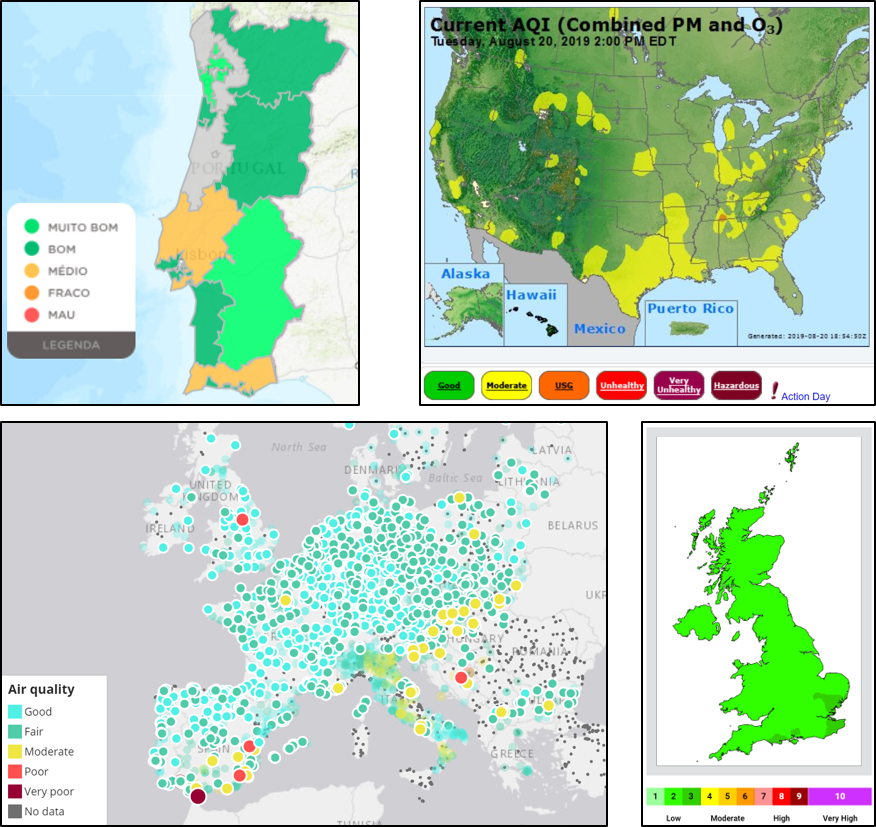
\includegraphics[width=0.65\textwidth]{./Images/air-visualization.png}
\caption{Governmental public online platforms for live air quality visualization.}
\label{fig:air-visualization}
\end{figure}

Reviewed governmental platforms in Europe and America, do not show fine interpolated data in their air quality maps. They only present, for each individual monitoring station, its local air quality index value. This leads to low resolution maps which are difficult to perceive and do not show air quality variances between stations. Some of these governmental platforms are presented in \Cref{fig:apa-stations-location}. At the top left is the QualAr platform, at the top right is the United States Environment Protection Agency one, at the bottom right is the air visualization provided by EEA, and at the bottom right is the platform provided by the United Kingdom government \cite{QualAr}\cite{U.S.EnvironmentProtectionAgency}\cite{EEA}\cite{DepartmentforEnvironment}.


Air quality visualization platforms from external companies to the government are business oriented and take advantage of the publicly available air quality data provided governments to make their live interpolated air pollution map as a product. Examples of these are Breezometer and AirVisual. These present heat maps with a much finer resolution than the ones provided by governments, as can be seen in \Cref{fig:breezo-visualization} \cite{Breezometer}. However, the spatial modelling algorithms used for the interpolation are proprietary, are not open-source and do not contribute to the literature, which is the aim of this work. Additionally, the accuracy provided from these is only extended to 500 meters \cite{Breezometera}.

\begin{figure}[ht]
\centering
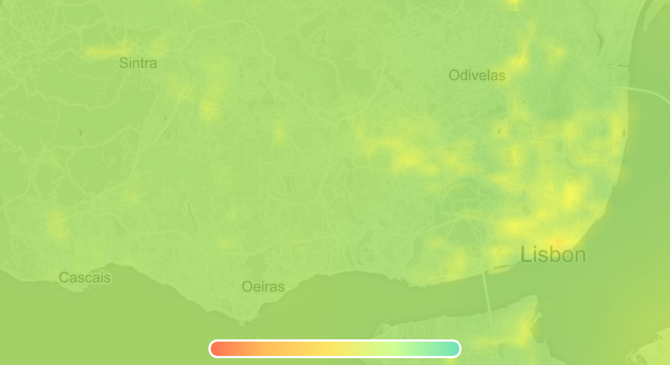
\includegraphics[width=0.6\textwidth]{./Images/breezo-visualization.png}
\caption{Breezometer high resolution live air quality map.}
\label{fig:breezo-visualization}
\end{figure}


%ler: https://blog.breezometer.com/accurate-air-quality-data
% https://blog.breezometer.com/understanding-air-quality-data
    
% #############################################################################
% If Printing on DOUBLE SIDED pages, the second page should be white.
% Otherwise, comment the following command:
\cleardoublepage
%
%Chapter 3
% #############################################################################
% This is Chapter 3
% !TEX root = ../main.tex
% #############################################################################
% Change the Name of the Chapter i the following line
\fancychapter{PM10 Monitoring, Interpolation and Visualization System}
\cleardoublepage
% The following line allows to ref this chapter
\label{chap:architecture}

%Reviewed literature has shown the current state of information available regarding urban air quality. The same can be said for the state of \ac{LPWAN} technology evolution and the current available and most used interpolation algorithms applied in the field of air quality spatial modelling. 

The methodologies and implementation details concerning the systems developed in this work are presented and explained in this section.

First, a small system that measures PM10 and retrieves them through NB-IoT to a server, which saves them in a database, was developed. This system consists of an NB-IoT module for communication and a PM low-cost sensor. Its performance was compared with one of the official standard PM sensors used by \ac{APA} in standard monitoring stations in Lisbon.

Second, SIMs were tested and assessed with the use of data from QualAr, from 2013 to 2017, with a focus on its comparison against FBNs, which have been shown to be promising when interpolating with sparse datasets \cite{Tome2014}.

Finally, a web application for the presentation of live high-resolution PM pollution rates was built, within a similar area to the city of Lisbon, covering the stations that provide data for the interpolations.

% #############################################################################
\section{Low Cost NB-IoT PM10 Monitoring System} 

The NB-IoT PM10 monitoring system was developed to evaluate how well these type of equipment could integrate current standard air monitoring networks, expanding its size, and consequently providing better data for spatial modelling approaches.

A low cost sensor was used to measure PM10 concentration in the air at a constant rate with relatively low power consumption. Sensor outputs were retrieved and processed by a programmable micro-controller.

The main requirements of this system were low production costs, a \ac{SFF}, low power consumption as well as long range transmission. A low bit rate is acceptable, since the measurement rate is also relatively low. The processing power required is low, since a low amount of data is processed by the micro-controller.

\subsection{Development and Composition}

NB-IoT was the LPWAN techology used in this work, due to the agreements between INESC-ID and Altice Portugal and NOS for its usage for research purposes, and considering the technology characteristics presented in \Cref{chap:back}.

\begin{itemize}[leftmargin=0.0mm]
  \item[] \textbf{SODAQ SARA SFF R412M}
\end{itemize}

\noindent
The development board used in this work is the SODAQ SARA SFF R412M board, which is an industry standard IoT developer board, with low power consumption, which allows the use of both NB-IoT and LTE-M networks, implying coverage across Europe, North America, Africa and Asia, with 62.5 kbit/s upload and 27.2 kbit/s download rates, and Over-The Air firmware updates \cite{U-blox}. This board contains an integrated micro-controller, the Atmel SAMD21, which allows it to be programmed through the same tools as every Arduino compatible board.

Subscriber identity module cards provided by the mobile operators NOS and Altice Portugal were used for this board remote communications with NB-IoT. These card were previously configured by the mobile operators according to the specifications needed for its optimal use in NB-IoT devices.

AT commands are used to communicate through the NB-IoT module. 
The commands used in the implementation of the developed system, and in the micro-controller program, along with its purpose are presented in \Cref{table:atCommands}. These are available in the SODAQ AT command manual \cite{U-Blox2018}.

\renewcommand\arraystretch{1.5}
\begin{table}[ht]
\centering
\caption{AT commands used with the NB-IoT micro-controller.}
\label{table:atCommands}
\begin{tabular}{l l} % centered columns (4 columns)
\toprule
Command&Functionality\\
\midrule
AT+CFUN&Sets the mobile terminal to full functionality\\
AT+CGATT&GPRS Attach\\
AT+USOCR&Create a socket\\
AT+USOST&Writes the specified amount of data to the remote address\\
AT+USOCL&Close socket\\
\bottomrule
\end{tabular}
\end{table}

The code developed for the micro-controller was written in the Arduino IDE environment, and consists of an internal loop that is continuously receiving measures from the sensor, and every 15 minutes, it makes the averages of the measures taken in that period and sends it through the NB-IoT AT commands, if there is network coverage.

The server code that receives the data from the NB-IoT modules is written in Python. In this program, an \ac{UDP} socket is used to receive packets from the sensor nodes. These contain the sensor location, id, a PM10 and a PM2.5 value, corresponding to the respective 15 minute averages. After receiving the data, it is stored in a database directly from the server.


\begin{itemize}[leftmargin=0.0mm]
  \item[] \textbf{Plantower PMS5003}
\end{itemize}

\noindent
A sensor from Plantower was used for the measurement of PM concentration, specifically the PMS5003, a low-cost light-scattering optical sensor with a built-in fan that provides air circulation, widely used and reviewed in the literature \cite{Kuula2019}\cite{Zheng2018}\cite{Zheng2019}\cite{Wendt2019}\cite{Ford2019}\cite{Manikonda2016}\cite{Liu2017}\cite{Sayahi2018}. This sensor measures both PM10 and PM2.5 concentration in suspended particles in the air, and outputs it through a digital signal, processed by a microprocessor, in real-time. Its minimum distinguishable particle diameter is 0.3 micrometers. Since it provides a low cost and low consumption profile, with an SFF, and also compatibility with Arduino boards, this sensor is optimal for this use case.


%A more detailed description of this sensor can be found in \cite{Yong2016}.

Its power supply requirements are 5V DC, and a maximum of 100mA. It can withstand operating temperatures from -10ºC to 60ºC, as well as relative humidity from 0 to 99\%. It is documented by the manufacturer that its maximum consistency error is of 10 μg/m³ if the measured values range from 0 to 100 μg/m³, and of 10\% from 100 to 500 μg/m³.

The PM sensor has two modes of functioning, the active and the passive mode. In the active mode, the sensor is always working and constantly sending digital data to the micro-controller. The data transport protocol works by sending 32 bytes periodically, of which each byte represents a different value. The first four and last four bytes are used for error checking. Bytes from 5 to 10 represent the PM concentration of suspended particles with the maximum diameter of 1, 2.5 and 10 respectively, for factory environments. Bytes from 11 to 16 have the same meaning, but in this is case for atmospheric environments. Finally, remaining bytes represent the number of particles with diameter beyond a certain value, which is a metric that is not in the scope of this thesis. This mode is depicted in \Cref{table:active-mode}.
In this work, only the bytes from 11 to 16 are of interest.

\renewcommand\arraystretch{1.5}
\begin{table}[ht]
\centering
\caption{Bytes in PMS5003 Active Mode functionality.}
\label{table:active-mode}
\begin{tabular}[t]{l>{\raggedright\arraybackslash}p{0.815\linewidth}}
\toprule
Byte Interval&Functionality\\
\midrule
1 to 4&Error check\\
5 to 10&PM10, PM2.5 and PM1.0 concentration under factory environment\\
11 to 16& PM10, PM2.5 and PM1.0 concentration under atmospheric environment\\
16 to 28&Number of
particles with diameter beyond 10, 5, 2.5, 1, 0.5 and 0.3 μm in 0.1 liters of air.\\
29 to 32&Error check\\
\bottomrule
\end{tabular}
\end{table}%


The passive mode is an host transport protocol, in which the micro-controller makes requests to the sensor and it replies accordingly. Due to the requirements on the sensor end, the active mode was the mode used in this work.


\begin{itemize}[leftmargin=0.0mm]
  \item[] \textbf{Step Up Voltage Converter}
\end{itemize}

\noindent
For the assembling of the SODAQ SFF R412M board with the PMS5003 sensor, a step up voltage converter is needed, since PMS5003 internal fan requires 5V DC power supply, and the SODAQ board can only output 3.3V. Despite this, the sensor high level of data pins is 3.3V. Therefore, the first iteration of this system can be presented as the one in \Cref{fig:ieec5}.


\begin{figure}[ht]
\centering
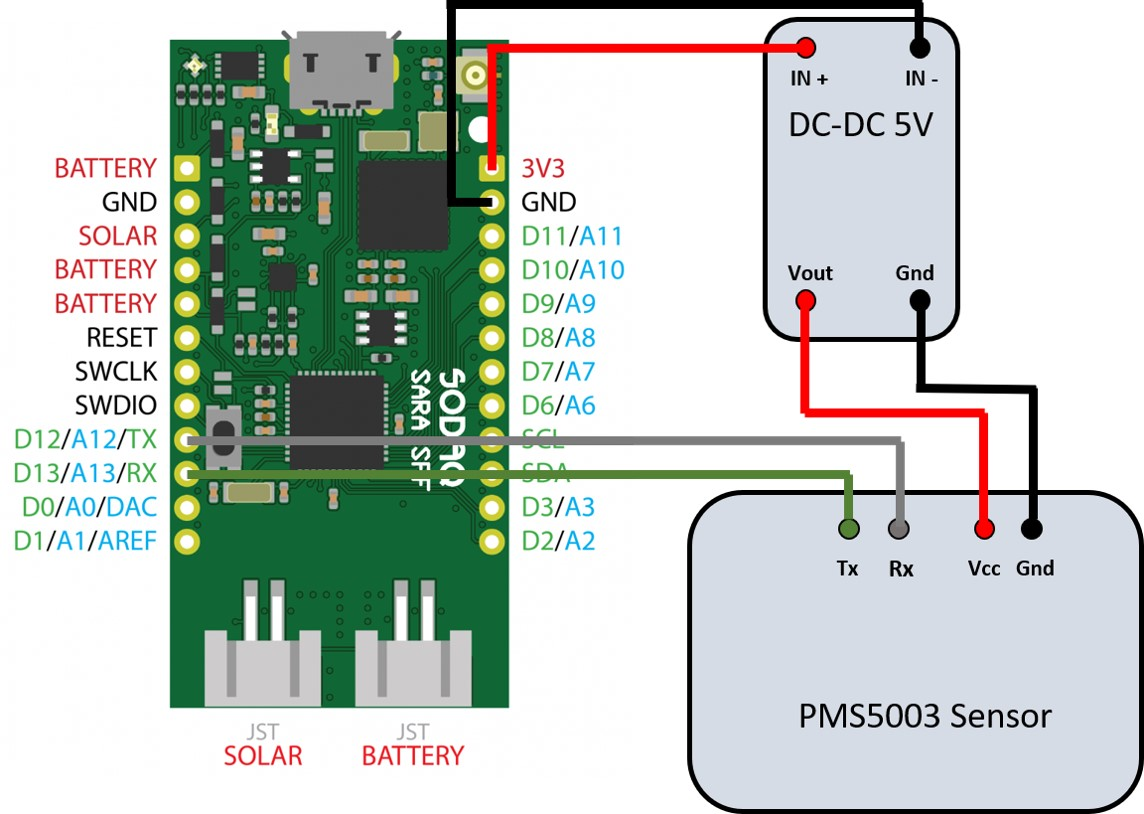
\includegraphics[width=0.6\textwidth]{./Images/ieec5.jpg}
\caption{First prototype of the developed PM monitoring system.}
\label{fig:ieec5}
\end{figure}

Similar to the behavior of the official monitoring networks, once data is collected from the sensors, 15 minute averages are calculated and sent to a server, which stores them in a database.

The developed system workflow is depicted in \Cref{fig:flowchart_monitoring_system}.

\begin{figure}[ht]
\centering
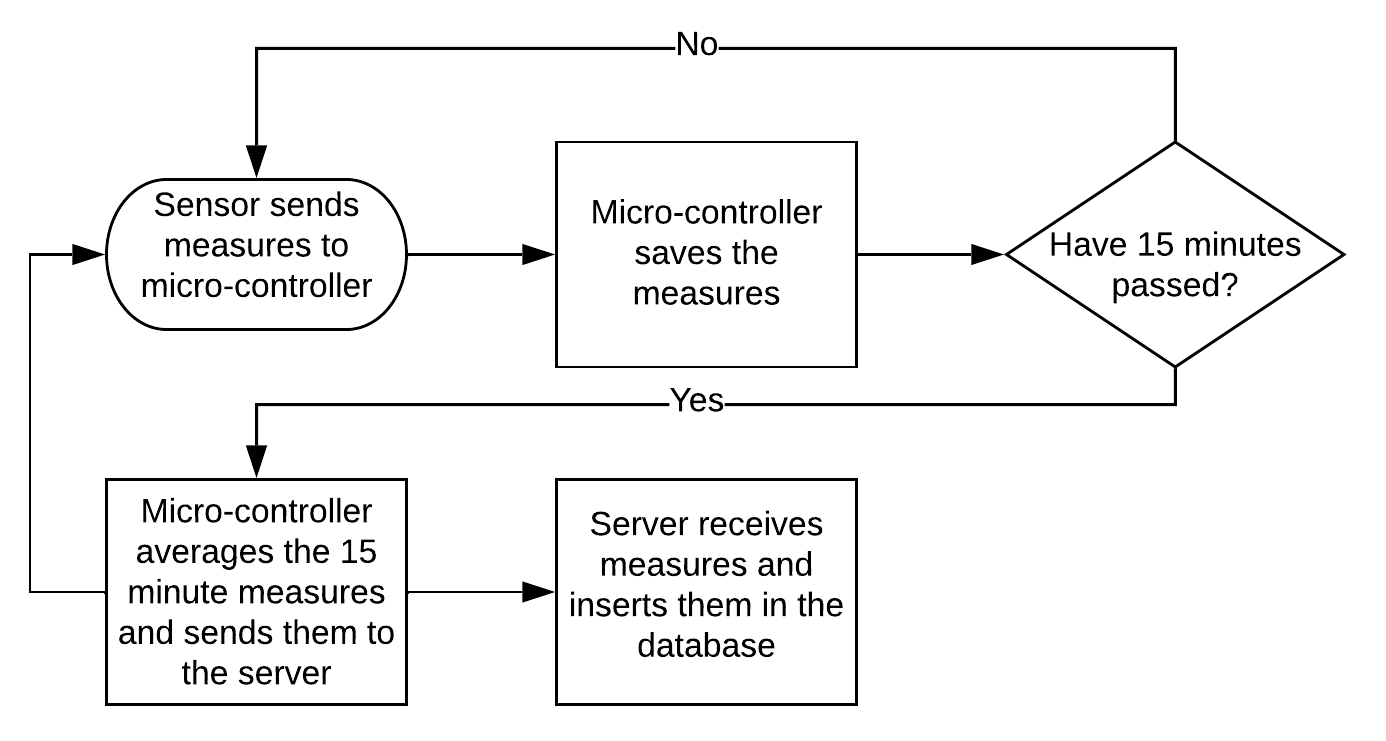
\includegraphics[width=0.75\textwidth]{./Images/flowchart_monitoring_system.png}
\caption{Overview of the developed monitoring system.}
\label{fig:flowchart_monitoring_system}
\end{figure}

\subsection{Placement and Behavior Analysis}

Both \ac{ENC} and the \ac{AVL} monitoring stations were used for the placement of the developed sensors.

Reference PM monitors are placed inside a container, and in order for air to reach the monitors, several teflon pipes are placed outside, within 2 meters of relative altitude, and the air is sucked through these pipes into the monitor container.

Similar behavior was intended to be replicated with the developed system with the junction of a vacuum pump and a plastic pipe to the developed system. However, to have better network coverage, the developed sensor had to be placed outside, in the top of the monitoring stations, next to the air entrance of the station and without any pipe, in a small box resistant to weather conditions and with an index of protection of 65. In \Cref{fig:circuit-final}, the final assembly of this system is presented.

\begin{figure}[ht]
\centering
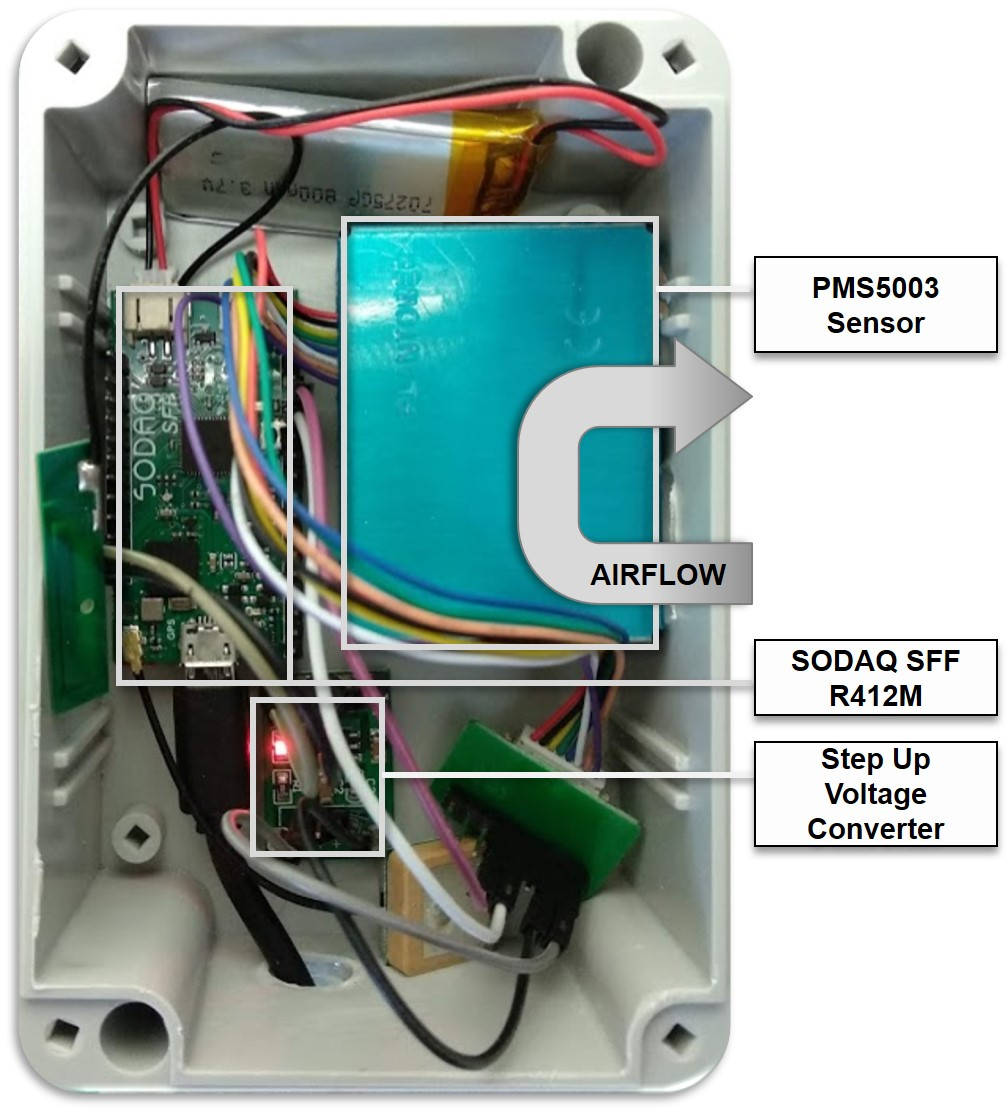
\includegraphics[width=0.45\textwidth]{./Images/circuit-final.jpg}
\caption{Final assembly of the developed monitoring system.}
\label{fig:circuit-final}
\end{figure}

%Aqui falta explicar que método será usado para fazer a calibração do sensor e talvez referênciar artigos onde esta técnica tenha já sido usada.
The developed system was placed during two weeks of July in AVL station, four weeks of August and two of September in ENC station and, finally, during the two final weeks of September in AVL station.

%\subsection{Functionality with SIMs}

%After the calibration process, based on the performance of the developed system in comparison to reference monitors, two main points can be made about it:

%\begin{enumerate}

%\item How low cost \ac{PM} monitors can be inserted in reference station networks in order to complement the data available to \ac{SIM}s, and also to help its assessment.

%The insertion of these type of systems in the current monitoring networks would greatly improve the spatial resolution of the data available for interpolation algorithms, which is crucial since the main obstacle in air quality spatial modelling is the low availability of data, as well as its sparsity.

%\item How low cost \ac{PM} monitoring systems perform against reference monitors with much higher purchase and maintenance costs.

%\end{enumerate}


% #############################################################################
\section{Spatial Interpolation Algorithms}

The main algorithms which are assessed in this work are FBN, OK and IDW. Additionally, simpler interpolation algorithms such as LI and NN are also tested. Data from 2005 to 2017 was extracted and analysed from QualAr website for the algorithms assessment. This data only concerns monitoring stations in the greater area of Lisbon,which corresponds to the area where air quality monitoring stations have the most spatial density in Portugal.

In this section, there is an overview of the data selection process, the algorithms parametrization and the tests that were done to assess the algorithms.

% Adicionar aqui informação se for possível fazer testes com algoritmos que levem em conta o tráfeog ou os ventos dominantes

\subsection{Dataset Selection}

In the greater area of Lisbon there is an air quality monitoring network composed of 14 monitoring stations, maintained by \ac{CCDR-LVT} \cite{QualAr}. Only 13 of these have operating PM10 sensors, from which only 10 are fully operating at the time of this work. Only 4 out of these have operating PM2.5 sensors. 

PM2.5 data was not regarded due to the lack of stations in the area of analysis. 

Only data from 2013 to 2017 was gathered since it is the most consistent overall, with measures from the considered stations, at high percentages of completeness (\Cref{table:completeness}).

From the five years of measures, a dataset of 43 506 hourly averaged measures was collected for each Lisbon PM10 measuring station. However, there were still many periods with incomplete data from some of the stations, since these were not working during certain periods. In order to remove data inconsistencies, the dataset was filtered based on the number of data per time interval. Each set was required to have at least 10 measures from all the considered stations, and at least 3 measures from the stations in the center of the network, presented in red in \Cref{fig:lx-stations-points}.

\begin{figure}[h]
\centering
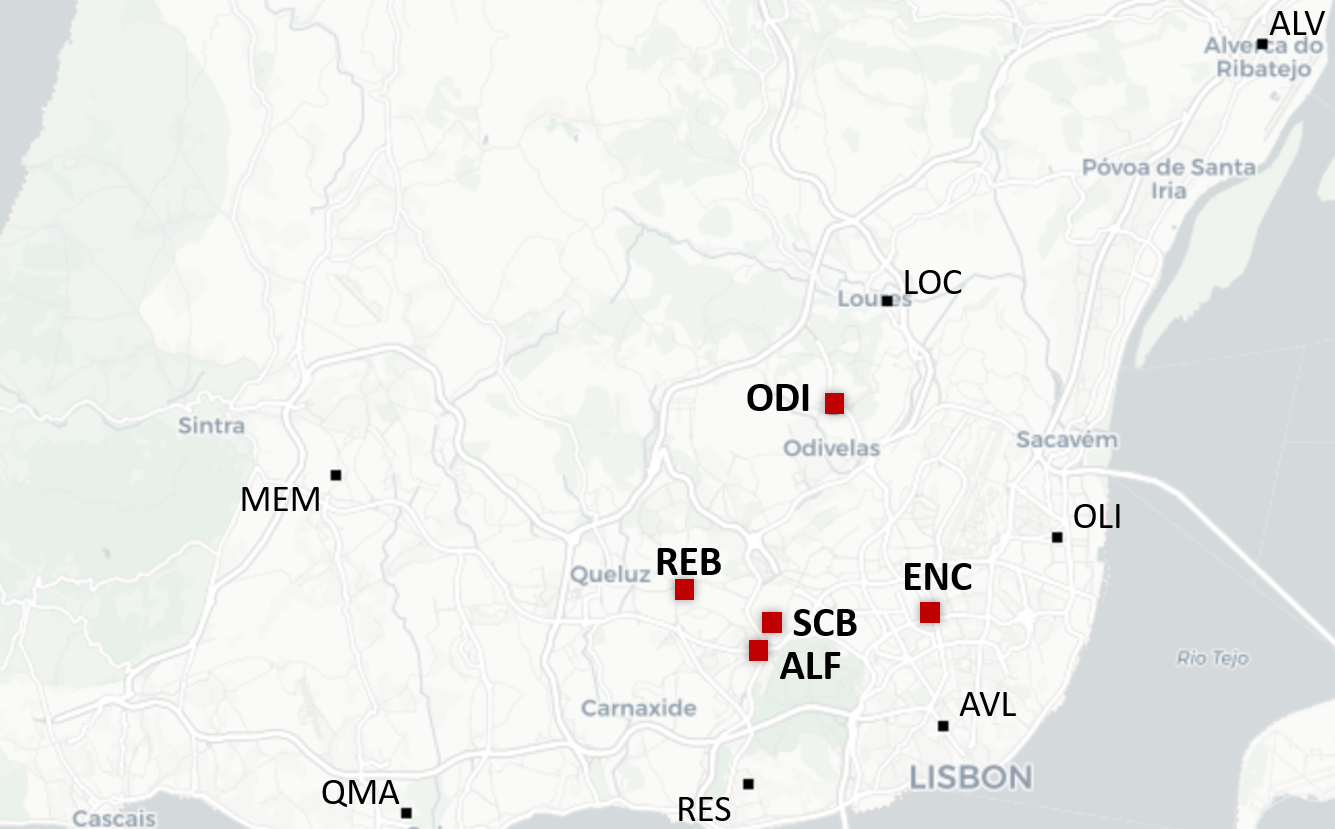
\includegraphics[width=0.7\textwidth]{./Images/lx-stations-points.png}
\caption{Considered stations in the greater area of Lisbon.}
\label{fig:lx-stations-points}
\end{figure}

In \Cref{table:completeness}, the percentages of completeness of each station before and after dataset filtering are presented. An increase of data completeness is evident in all stations. The \ac{ALF} station demonstrated very low completeness overall, before and after filtering, therefore it was removed from the dataset.

\renewcommand{\tabcolsep}{3pt}
\renewcommand\arraystretch{1.1}
\begin{table}[ht]
\centering
\caption{PM10 data completeness of considered stations before and after data filtering.}
\label{table:completeness}
\begin{tabular}{p{0.22\textwidth}>{\centering}p{0.08\textwidth}>{\raggedright}p{0.15\textwidth}>{\centering}p{0.15\textwidth}>{\centering}p{0.15\textwidth}>{\centering\arraybackslash}p{0.1\textwidth}}
\toprule
\multirow{2}{*}{Station}&\multirow{2}{*}{ID}&\multirow{2}{*}{Station Type}&\multirow{2}{*}{Area Type}&\multicolumn{2}{c}{Data Completeness (\%)}\\\cline{5-6}
&&&&Overall&Filtered\\
\midrule
Alfragide/Amadora&ALF&Background&Urban&1.40&2.85\\
Alverca&ALV&Background&Urban&97.47&99.96\\
Avenida da Liberdade&AVL&Traffic&Urban&96.49&99.21\\
Entrecampos&ENC&Traffic&Urban&76.40&99.50\\
Loures-Centro&LOC&Background&Urban&85.88&91.46\\
Mem Martins&MEM&Background&Urban&88.31&99.72\\
Odivelas-Ramada&ODI&Traffic&Urban&82.89&98.88\\
Olivais&OLI&Background&Urban&93.74&99.54\\
Quinta do Marquês&QMA&Background&Urban&89.30&99.55\\
Reboleira&REB&Background&Urban&68.88&96.88\\
Restelo&RES&Background&Urban&29.66&40.81\\
Santa Cruz de Benfica&SCB&Traffic&Urban&48.67&82.00\\
\bottomrule
\end{tabular}
\end{table}%

The \ac{ALV} station was also removed from the dataset, because it is located too far from the center stations, which would increase the problem sparsity and possibly degrade the algorithm performance. This data exclusion process can be observed in \Cref{fig:dataset-filtering}, where \textit{N} represents the size of each dataset.

\begin{figure}[ht]
\centering
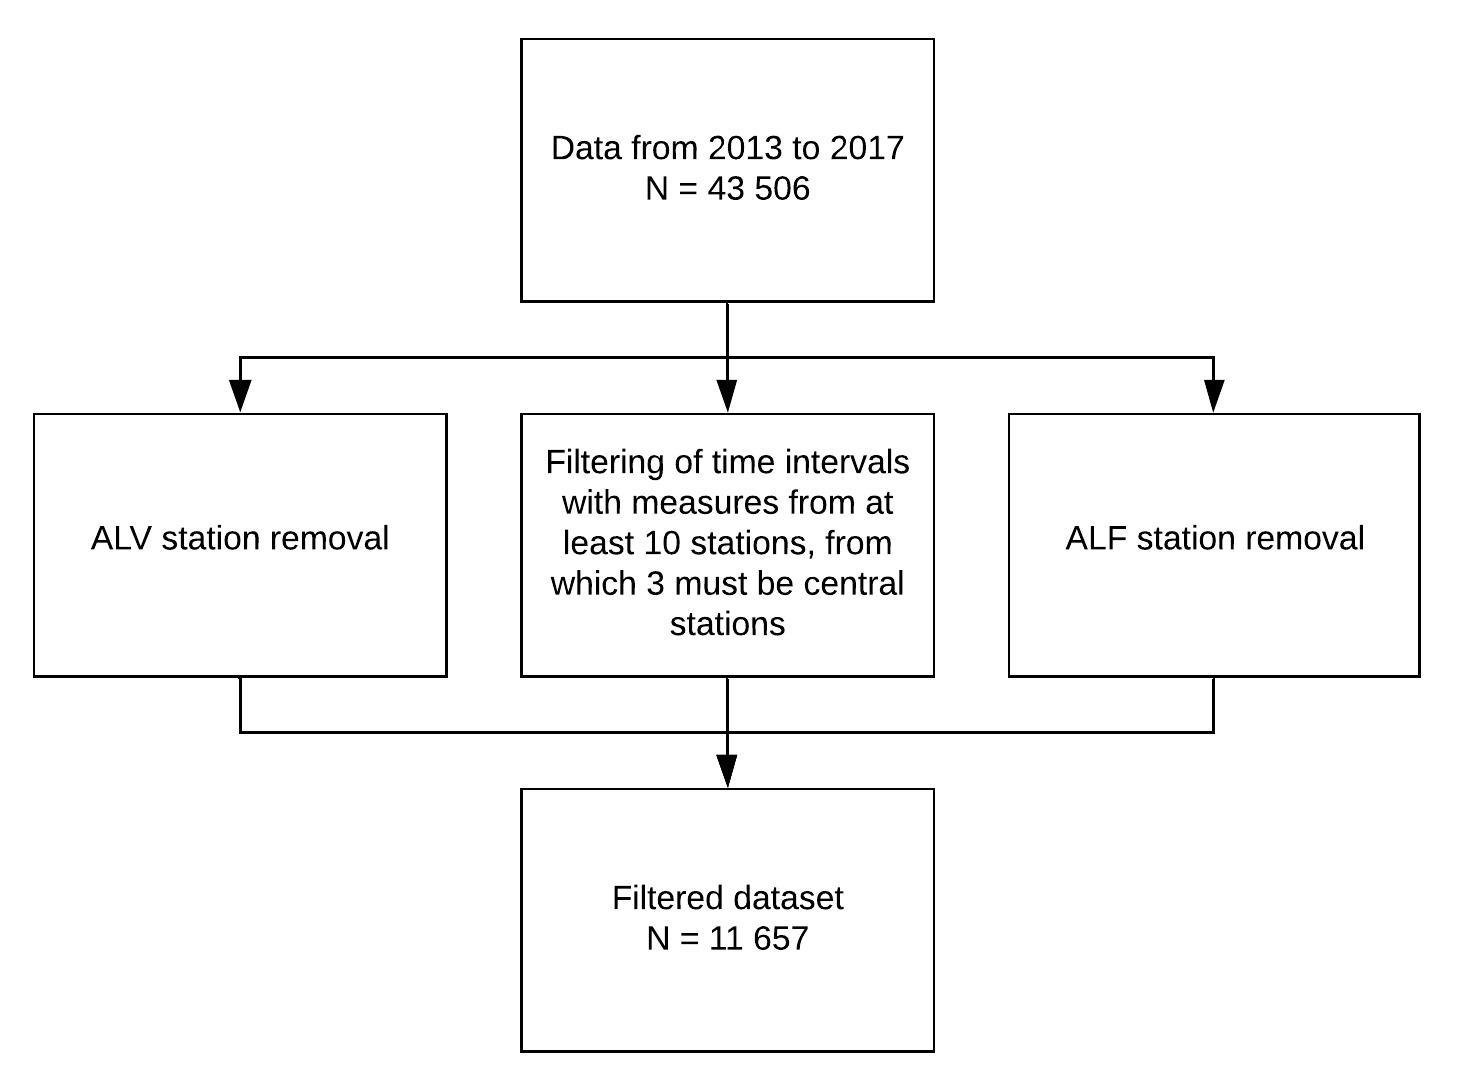
\includegraphics[width=0.8\textwidth]{./Images/dataset-filtering.jpeg}
\caption{Dataset exclusion process.}
\label{fig:dataset-filtering}
\end{figure}

The number of sets of measures in the dataset decreased from 43 506 measures in the initial dataset, to 11 657 in the filtered one. A map with the remaining Lisbon monitoring stations, after dataset filtering, is presented in \Cref{fig:map-filtered}. 

Data correlation was also calculated between every station and the center target stations. These coefficients help to explain the quality of the spatial prediction obtained by the various models. In \Cref{table:correlation-coef} these are presented, with an highlight of the stations which share higher linear correlation.

%\renewcommand{\tabcolsep}{3pt}
\renewcommand\arraystretch{1}
\begin{table}[h]
\centering
\caption{Correlation coefficient between target and remaining stations in the Lisbon monitoring network.}
\label{table:correlation-coef}
\begin{tabular}[t]{l>{\centering}p{0.1\linewidth}>{\centering}p{0.1\linewidth}>{\centering}p{0.1\linewidth}>{\centering\arraybackslash}p{0.1\linewidth}}
\toprule
&ENC&ODI&REB&SCB\\
\midrule
%ALF&1&0.53&0.47&0.42&0.54\\
%ALV&0.76&0.78&0.79&0.69\\
AVL&0.83&0.77&0.78&0.76\\
ENC&1&0.84&0.82&\textbf{0.81}\\
LOC&0.77&0.79&0.79&0.69\\
MEM&0.77&0.78&0.8&0.66\\
ODI&\textbf{0.84}&1&\textbf{0.86}&0.78\\
OLI&0.83&0.76&0.78&0.74\\
QMA&0.77&0.78&0.83&0.71\\
REB&0.82&\textbf{0.86}&1&0.8\\
RES&0.76&0.83&0.81&0.73\\
SCB&0.81&0.78&0.8&1\\
\bottomrule
\end{tabular}
\end{table}%

These were calculated with the Pearson correlation coefficient, which has been used in similar applications \cite{Deligiorgi2011}, and represents the linear correlation between two variables. 
The possible result values vary from 1 to -1, where 1 represents total positive linear correlation, 0 represents no linear correlation, and -1 total negative linear correlation.

\begin{figure}[ht]
\centering
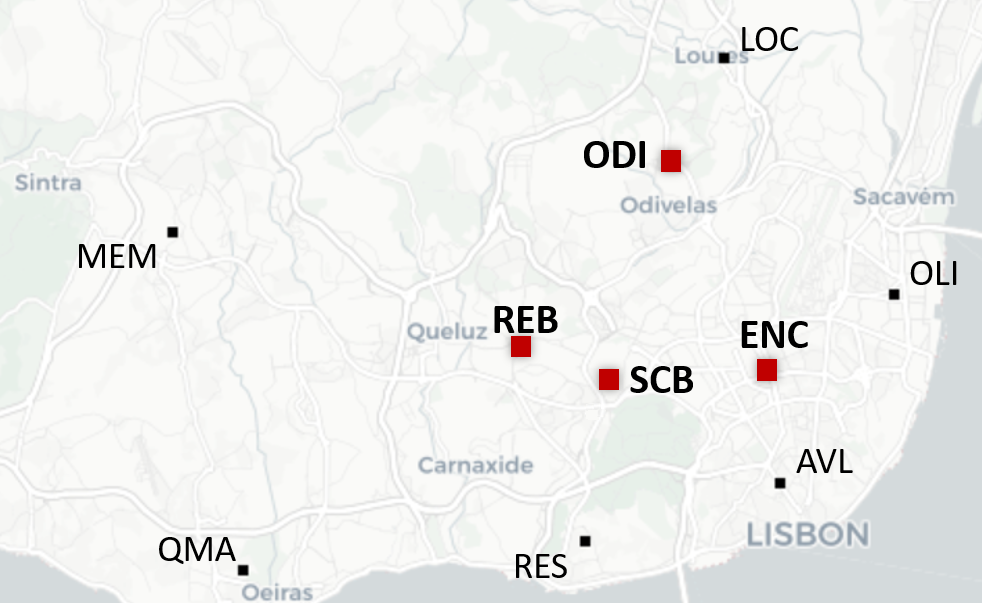
\includegraphics[width=0.7\textwidth]{./Images/map-filtered.png}
\caption{Stations in the greater area of Lisbon used in this work.}
\label{fig:map-filtered}
\end{figure}

\subsection{Spatial interpolation Algorithms Implementation}

In order to assess algorithm performance, cross validation tests were applied to the selected stations. In each iteration, one measure from one central station (\Cref{fig:map-filtered}) was inferred using the measures from remaining stations in the same time interval. In \Cref{main-pseudocode} the pseudo-code of the setup of this process is presented.

\begin{center}
\begin{algorithm}[H]
\linespread{1.35}\selectfont
\SetAlgoLined
 dataset = extractDataset()\;
 stations = stationsData()\;
 centralStations = centralStationsData()\;
 \ForEach{set in dataset}{
  \ForEach{station in stations}{
   \If{station in centralStations}{
    executeInterpolationAlgorithms(station, set)\;
   }
  }
 }
 \caption{Pseudo-code of the algorithm execution setup.}
 \label{main-pseudocode}
\end{algorithm}
\end{center}

Both LI and NN were implemented with the python \textit{scipy} library \textit{interpolate} package.

In what regards IDW, its only user defined parameter is the power function value \textit{p}, which defines how the weight of each observed point varies with the distance to the estimated point. This algorithm was implemented in Python.
Cross validation was applied to decide which is the best value of \textit{p} for the selected data.

OK is the Kriging variant which was considered in this work, and it was implemented with the \textit{pykrige} python library \cite{PyKrige2019}.

Variograms can only be modelled if datasets have a relative high number of points and spatial density, which is not the case in this work, in which observation points are only 10 and sparsely distributed \cite{Mesquita2009}.
Cross validation was applied to decide which is the best Kriging variogram for this work selected data.

\subsection{FBN Implementation}

FBNs have several implementation details which are user defined.

\begin{itemize}[leftmargin=0.0mm]
  \item[] \textbf{Antecedent and Consequent Areas}
\end{itemize}

\noindent
First, the amount of antecedent and consequent areas that constitute the network, and which variables are associated to each area, must be defined. The dataset PM10 values and its coordinates are the variables used. The interpolation objective is to model a value for the PM concentration at a specific location, with a respective pair of coordinates. Therefore, there are two independent variables, represented as antecedent areas - latitude and longitude - and one unknown value, represented as consequent area - PM10 concentration.

\begin{itemize}[leftmargin=0.0mm]
  \item[] \textbf{Variables Scale Conversion}
\end{itemize}

\noindent
Since each area only receives inputs between 0 and 1, the values of all used variables (latitude, longitude and PM10 concentration) need to be converted to the same scale, and a maximum value needs to be defined, to represent 100\% ratio of its corresponding area.

In the case of the coordinates, delimiting values were represented by the outline of the most exterior stations. 

The station at the extreme west location is \ac{MEM} whose longitude is -9.347222, and the extreme east station is \ac{OLI} with a longitude of -9.108056. Therefore, the longitude defined value for 0 is -9.35 and for 1 is -9.1.

The same was done for the latitude. The southest station is \ac{QMA}, which has latitude equal to 38.6975, and the northest is \ac{LOC} whose latitude is 38.829722. Therefore, the defined values for 0 and 1 for the antecedent area corresponding to the latitude coordinate are 38.69 and 38.83 respectively.

With these settings it is possible to define the spatial grid presented in \Cref{fig:scale-converted-grid}.

\begin{figure}[ht]
\centering
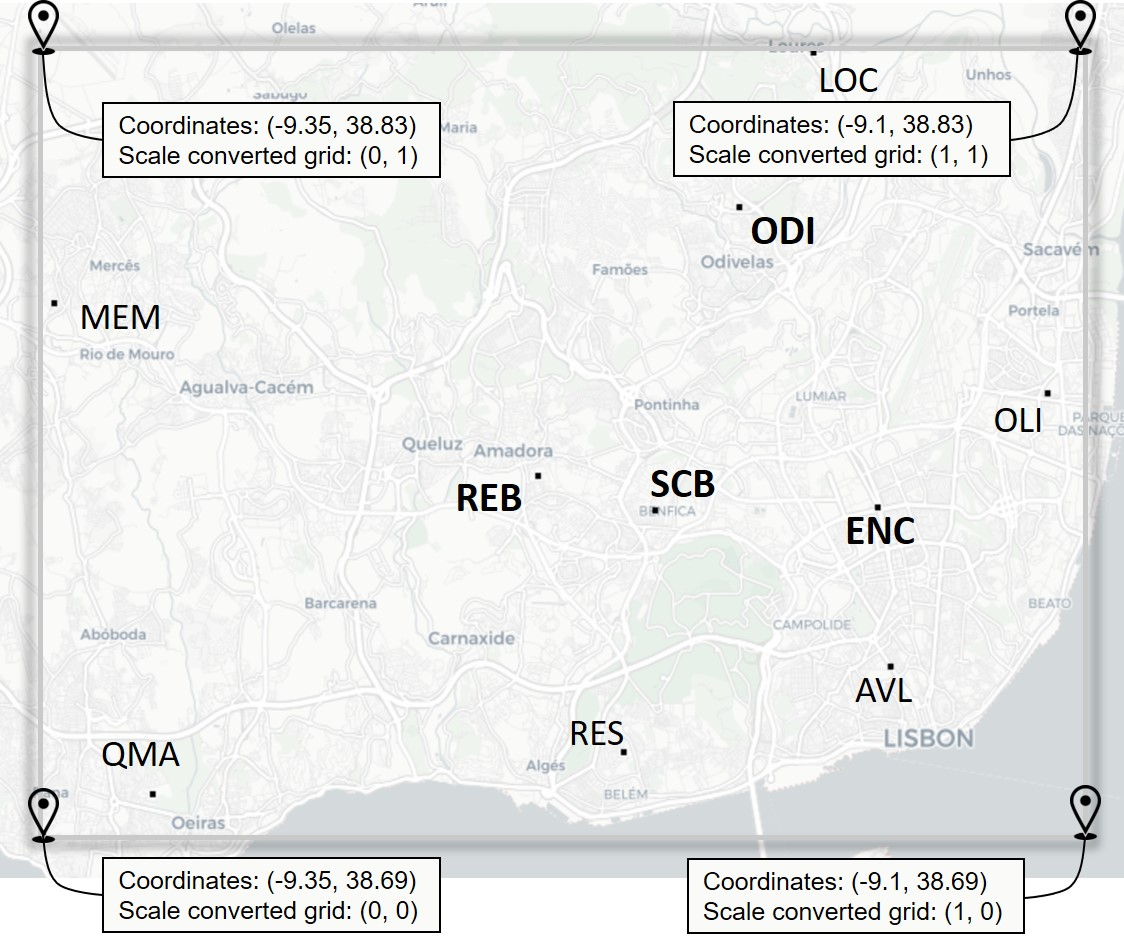
\includegraphics[width=0.8\textwidth]{./Images/scale-converted-grid.jpg}
\caption{Spatial grid used for FBN coordinate scale conversion.}
\label{fig:scale-converted-grid}
\end{figure}

Finally, for the PM10 concentration values, the minimum value was 0 μg/m³ and the maximum value was 175 μg/m³, which is above the highest registered value in the filtered 5 year dataset.

The equations from \Cref{longitude} to \Cref{pm10-concentration} represent the scale transformations used for each variables, longitude, latitude and PM10 concentration.

\begin{equation} 
\label{longitude}
\scalebox{1.4}{$ Lon_{val} = \dfrac{Lon_{station}-Lon_{min}}{Lon_{max}-Lon_{min}} $}
\end{equation}

\begin{equation} 
\label{latitude}
\scalebox{1.4}{$Lat_{val} = \dfrac{Lat_{station}-Lat_{min}}{Lat_{max}-Lat_{min}}$}
\end{equation}

\begin{equation} 
\label{pm10-concentration}
\scalebox{1.4}{$PM10_{val} = \dfrac{PM_{observed}}{175}$}
\end{equation}

%As already noted, the ALV station was excluded from the dataset due to its farther location compared to every other station. Both its longitude and latitude coordinates would represent extreme values to the scale transformation which could be detrimental to FBN execution, since it would decrease the data spatial density, namely the latitude maximum value would increase significantly the respective axis scale.

\begin{itemize}[leftmargin=0.0mm]
  \item[] \textbf{Parametrization}
\end{itemize}

\noindent
In order to better explain and understand FBN performance in this work application, several parametrizations were tested.
The user defined parameters which were tested are the number of antecedent and consequent areas in the network, the number of testing and training epochs, the granularity and the number of samples.

Training and testing epochs were tested on how its increase, independently of the network size, influences results. Furthermore, net size along with number of samples and granularity were also tested to conclude how these parameters can provide a better accuracy against time of execution through cross validation in the selected dataset.

In order to analyse how resolution of data influences FBNs interpolation performance results, these were tested with a dataset of 15 minutes intervals values measured at monitoring stations. This dataset was provided by CCDR-LVT, and contained only measures from the stations AVL, ENC, OLI, RES and SCB.

Additionally, FBNs were tested with data from four 15 minute sets of values per hour, to infer an average for that hour at the location of each station. This was different than previous tests, in which only hourly averages were used to train and were infered by FBNs.

%OK, IDW and FBNs were executed with the hourly average sets for the corresponding period, as a control measure of increases in performance between FBN executions. Afterwards, FBNs were solely trained with the 15 minutes intervals. The only difference between both FBN implementations, is the number of training sets. In the implementation which received only hour averages as inputs, there was only one set of training sets for each interpolation. In the implementation with 15 minutes measures, there were 4 training sets.


\begin{itemize}[leftmargin=0.0mm]
  \item[] \textbf{Implementation}
\end{itemize}

\noindent
The implementation of FBN was the result of previous works \cite{Tome2014}. This implementation was migrated from Python 2 to Python 3, and code was additionally developed to insert every training and testing rule in the networks directly from an excel dataset. This enables the interpolation of several datasets in only one execution.

%One of the goals of this work is to experiment and compare \ac{FBN}s performance against state-of-the-art algorithms for the spatial interpolation of air pollution, namely \ac{PM10} and \ac{PM2.5}, such as Kriging and \ac{ANN} based models. For this its better parameters need to be defined. This will be made through the use of the cross validation technique further explained in the following section.

%FBN functioning was already explained in section XX, therefore it is known that for its implementation several parameters need to be previously assessed and defined in order to get the best results possible with the lowest amount of execution time.
%These parameters are the number of samples, …
%Several tests with the data explained above will be made in this study in order to define the best parameters for this problem.

%In the original implementation of FBNs, several files need to be previously written with the details of the details, specifications and user defined parameters of the FBN.

%the rules of the learning and the training process which consist of…

%and the data for the inference process which consists of…

%In order to systemize this, a python program was developed to write these files automatically without the need to write these files.
%This program reads the training data directly from the excel provided by APA in the case of the hourly data, or the excel filled by the pre mentioned python program with the quarter of an hour data, the user can define the fbn parameters directly in the code, and the program further produces the files needed for the FBN execution.
%The 15 to 15 data provided by the CCDR-LVT were presented in a normal text file with no specific format. A python program was made to export these to excel, for them to be used by the above systematic program.

\subsection{Algorithm Performance Evaluation}

In order to assess the results of the cross validation approach, the statistical error parameters presented in equations \eqref{mae} and \eqref{rmse} were considered.

\begin{equation} 
\label{mae}
\scalebox{1.4}{ $ MAE = \dfrac{\sum_{i=1}^{n} |M_i - O_i|}{n}$}
\end{equation}

\begin{equation} 
\label{rmse}
\scalebox{1.4}{ $ RMSE = \sqrt[2]{\dfrac{1}{n}\sum_{i=1}^{n} {(M_i - O_i)}^{2}}$}
\end{equation}

%\begin{equation} 
%\label{r2}
%\scalebox{1.4}{ $ {R}^{2} = 1 - \dfrac{\sum_{i=1}^{n} {(O_i %- M_i)}^{2}}{\sum_{i=1}^{n} {(O_i - \overline{O_i})}^{2}}$}
%\end{equation}

Where $M_i$ represents the modelled value, $O_i$ represents the observed value and $n$ is the total of inferences.% and $\overline{O_i}$ is the mean of the observed values.

\ac{MAE} measures the average magnitude of errors in a set of predictions. \ac{RMSE} is a quadratic parameter which also measures the average magnitude of the error.
Both express average model prediction error in units of the variable of interest, which for PM10 concentration are μg/m³. Regarding RMSE, since errors are squared before they are averaged, increased weight is given to large errors.

%${\textrm{R}}^{2}$ is a statistical measure that represents the proportion of the variance of a dependent variable that is explained by the independent variables. 

%According to directive 2008/50/EC, the measure of the uncertainty

%max uncertainty is 25\%.
%uncertainty = (observed value - modelled value)/ limit value
%averaging period one day: 50 μg/m3
%calendar year: 40

%\begin{equation} 
%\label{uncertainty}
%\scalebox{1.3}{$ uncertainty = \dfrac{O - M}{limit\: value} $}
%\end{equation}

%Where $M$ is the modelled value, 

% #############################################################################
\section{System for Online Data Visualization} 

The system for online data visualization is composed of a database, an html, css and javascript apache website with a javascript library which provides custom map web visualization and rendering, Mapbox GL JS.

\subsection{Database}

A MongoDB database was developed to store the values obtained by monitoring systems. Depending on the performance of the developed low-cost system, several of its replicas could be placed around Lisbon, in locations where there are no other monitoring stations, in order to complement and increase the density of data for the city of Lisbon.

MongoDB was the database technology chosen for this specific application, due to its high scalability and flexibity. It is a NoSQL type of database, which stores data in flexible, JSON-like documents. It is a distributed database at its core, therefore it has high availability through built-in replication, and horizontal scalability with native sharding, with end-to-end security. Each database contains collections, which in turn contain documents. Documents are filled with fields and the size and content of documents in the same collection can vary.

The database used in this work only has one collection, in which every measure from the system is saved. Despite the non-enforcement of document structure in the database, for the purpose of this work, each valid document must have date, location, sensor ID and pm10 value as valid fields, and the date field along with the sensor ID can not be repeated in different documents.

\subsection{Mapbox GL JS}

Mapbox is a provider of custom online maps for websites and applications. The company was founded in 2010 and has contributed to, and created, several tools which let developers use custom maps in their own platforms. It has emerged as a response to the limited choice offered by map providers such as Google Maps. Some of these tools are open source mapping libraries and applications, such as the Mapbox GL JS JavaScript library, the MBTiles specification, the TileMill cartography IDE, the Leaflet JavaScript library and the CartoCSS map styling language and parser \cite{Mapbox2019}.

Mapbox GL JS is a JavaScript library which uses WebGL to render interactive maps from vector tiles and Mapbox styles, and it was used in this work to represent the results of the real-time spatial interpolation PM10 values.

Its online map implementations are widely customizable and allow the visualization of a wide variety of data representations in the chosen map, such as polygons, icons, buildings, polygons, 3D models and animations.

In this work, extrusion of polygons was used to represent the levels of estimated PM10 concentration values, whose height and color is determined by the pollution value in each point of the map.

For the representation of these polygons, a grid was defined, which is delimited by the coordinates of the Lisbon monitoring station networks which are on the edges of the city. This is a convex hull grid, with a resolution of 100 m². For these extrusions to be included, a geojson file was created, with the polygons of every element in the defined grid. A python script is running in the background which updates the values at each station every hour, performs a new interpolation with the updated values, and updates the geojson file accordingly.

Regarding the javascript implementation, a Map object, which represents the whole map visualization, is defined in the main website file. In the javascript code of the webpage, the geojson file, which should be saved in a local directory, is accessed, and then its respective extrusions are inserted in the Map object, which is rendered when users access the webpage.

%\subsection{API}

% Ideally there should be an API - Ou então dizer que é apenas um servidor Apache
% The part about the python script needs to be changed once this change is % done.

% #############################################################################
% If Printing on DOUBLE SIDED pages, the second page should be white.
% Otherwise, comment the following command:
\cleardoublepage
%
%Chapter 4
% #############################################################################
% This is Chapter 4
% !TEX root = ../main.tex
% #############################################################################
% Change the Name of the Chapter i the following line
\fancychapter{Results}
\cleardoublepage
% The following line allows to ref this chapter
\label{chap:implement}

In this chapter, the results regarding the overall developed system for air quality monitoring and visualization with NB-IoT will be presented, as well as the performance of the considered SIMs. It will be divided into four sections, the PM10 Monitoring System experiment, SIMs performance, Online Data Visualization Web Application and finally Discussion. In this final section, the obtained results are addressed and analyzed in terms of what substantial inferences can be made regarding the experiments of this work.

For a better understanding of the results, it is important to note how PM10 concentrations affect air quality.
In \Cref{table:pm10-classification} one can see the official classification of the PM10 concentration values \cite{QualAr}.

\definecolor{springgreen}{rgb}{0.0, 0.65, 0.31}
\definecolor{carrotorange}{rgb}{0.93, 0.57, 0.13}
\definecolor{electricgreen}{rgb}{0.0, 1.0, 0.0}
\definecolor{bostonuniversityred}{rgb}{0.8, 0.0, 0.0}
\begin{table}[ht]
\centering
\caption{Classification of PM10 concentration values.}
\label{table:pm10-classification}
\begin{tabular}[t]{>{\centering}p{0.13\linewidth}>{\centering\arraybackslash}p{0.4\linewidth}}
\toprule
Classification&PM10 concentration interval (μg/m³)\\
\midrule
\cellcolor{electricgreen}Very Good& 0 - 20\\
\cellcolor{springgreen}Good& 21 - 35\\
\cellcolor{yellow}Medium& 36 - 50\\
\cellcolor{carrotorange}Weak& 51 - 100\\
\cellcolor{red}Bad& 101 - 1200\\
\bottomrule
\end{tabular}
\end{table}%

It can be observed that the smallest classification interval corresponds to a 14 μg/m³ variation, for both Good and Medium intervals. 
This value is useful to assess overall error results in relation to official metrics, for both the assessment of SIMs and the errors of measures between the developed system and reference monitors.


% #############################################################################
\section{NB-IoT PM10 Monitoring System}

This section objective is to describe the developed monitoring system performance and measures in comparison to the reference monitors, to later assess how it may integrate existing reference monitoring networks, which lack geographical density. Furthermore, the state and performance of the NB-IoT technology during the period of its use in this work is characterized.

\subsection{NB-IoT Coverage in Lisbon}

In \Cref{table:measurement-period} are presented the weeks during which the developed system was placed in a CCDR-LVT station. Colored cells represent the location where the developed sensor was placed during each week. In weeks colored in green, consistent measures were taken since there was NB-IoT coverage. On the other hand, in red colored weeks it was impossible to get consistent coverage and consequently no measures were obtained.

\definecolor{springgreen}{rgb}{0.0, 0.65, 0.31}
\definecolor{bostonuniversityred}{rgb}{0.8, 0.0, 0.0}
\renewcommand\arraystretch{1.5}
\renewcommand{\tabcolsep}{3pt}
\begin{table}[ht]
\centering
\caption{Weeks during which the developed system was placed next to a CCDR-LVT monitoring container.}
\label{table:measurement-period}
\begin{tabular}[t]{l>{\centering}p{0.06\linewidth}>{\centering}p{0.06\linewidth}>{\centering}p{0.06\linewidth}>{\centering}p{0.06\linewidth}>{\centering}p{0.06\linewidth}>{\centering}p{0.06\linewidth}>{\centering}p{0.06\linewidth}>{\centering}p{0.06\linewidth}>{\centering}p{0.06\linewidth}>{\centering\arraybackslash}p{0.06\linewidth}}
\toprule
&\multicolumn{2}{c}{July}&\multicolumn{4}{c}{August}&\multicolumn{4}{c}{September}\\
\midrule
{}Week&3&4&1&2&3&4&1&2&3&4\\
\midrule
AVL&\cellcolor{bostonuniversityred}&\cellcolor{bostonuniversityred}&&&&&&&\cellcolor{springgreen}&\cellcolor{springgreen}\\
ENC&&&\cellcolor{bostonuniversityred}&\cellcolor{bostonuniversityred}&\cellcolor{bostonuniversityred}&\cellcolor{bostonuniversityred}&\cellcolor{bostonuniversityred}&\cellcolor{bostonuniversityred}&&\\
\bottomrule
\end{tabular}
\end{table}

%%%%%%%%%%%%%%%%%%%%%%%%%%%%%%%%%%%%%%%%%%%%%%%%%%%%%%%%%%%%

\subsection{Evaluation of Obtained Measures}

From 13 to 26 September, measures obtained for each 15 minute interval were consistent and valid. The resulting data characteristics from these during this period are presented in \Cref{table:data-calibration-characteristics}.

\begin{table}[ht]
\centering
\caption{Data obtained during the measurement period.}
\label{table:data-calibration-characteristics}
\begin{tabular}[t]{>{\centering}p{0.13\linewidth}>{\centering}p{0.3\linewidth}>{\centering\arraybackslash}p{0.32\linewidth}}
\toprule
Full days&Obtained measures& Resulting hourly averages\\
\midrule
12&1195&298\\
\bottomrule
\end{tabular}
\end{table}%

Since data available from the reference monitor only corresponded to hourly averages, these were also calculated for the data obtained from the developed sensor, for comparison purposes. It is important to note that the reference monitor averages available online \cite{QualAr} are made for each hour with all the 15 minute spaced measures from the previous hour. Therefore, the same process was applied to calculate the developed system averages.

Statistics, such as the mean value, standard deviation and maximum and minimum values, regarding both obtained data sets were calculated and are presented in \Cref{table:error-measurement-period}.

\renewcommand\arraystretch{1.1}
\renewcommand{\tabcolsep}{1.4pt}
\begin{table}[ht]
\centering
\caption{Results of the measurement period, in (μg/m³).}
\label{table:error-measurement-period}
\begin{tabular}[t]{l>{\centering}p{0.15\linewidth}>{\centering}p{0.2\linewidth}>{\centering}p{0.2\linewidth}>{\centering\arraybackslash}p{0.2\linewidth}}
\toprule
{} &Mean value&Standard Deviation&Maximum value&Minimum value\\
\midrule
Reference Monitor&27.88&8.78&55.00&8.00\\
Developed System &15.04&10.64&56.80&2.49\\
\bottomrule
\end{tabular}
\end{table}

In \Cref{fig:system-calibration}, simultaneous measures of both sensors can be observed, for the whole time of placement of the developed system, along with the average RH values for the city of Lisbon.

\begin{figure}[ht]
\centering
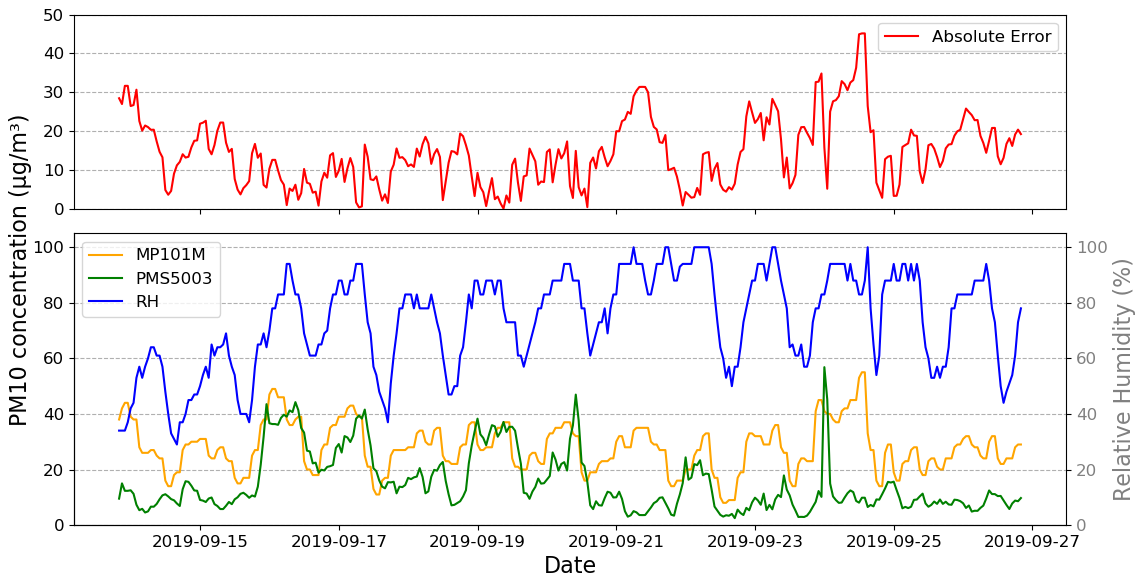
\includegraphics[width=1\textwidth]{./Images/Results/calibration2.png}
\caption{Time series of the PM10 concentrations reported by the sensors and corresponding RH.}
\label{fig:system-calibration}
\end{figure}

Several tendencies can be observed. The PMS5003 sensor often obtained lower measures. However, sometimes it peaked, surpassing the MP101M measures. This only happens for high values of RH. When the RH is decreasing, there is often less error between sensors.


The days 14, 15, 21 and 22 of September corresponded to weekend days, which means there is less car traffic in AVL. No meaningful tendencies were observed in these days, despite the average PM10 concentration being slightly lower in both sensors.

The average absolute error between the measures of the different sensors is 14.40 μg/m³. Furthermore, the scatter diagram in \Cref{fig:scatter-measurements} also highlights that the developed system measured values are predominantly lower than the reference measures.

\begin{figure}[ht]
\centering
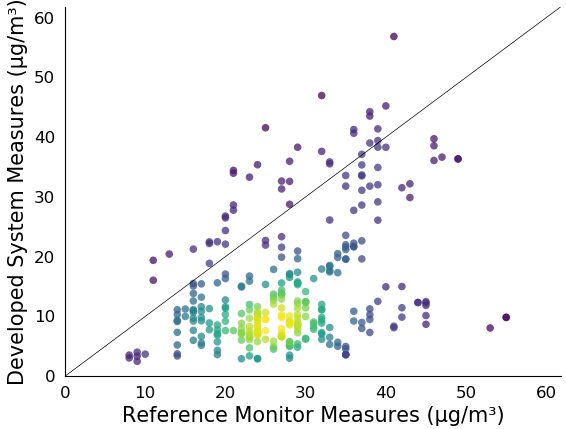
\includegraphics[width=0.55\textwidth]{./Images/Results/scatter-measurements.png}
\caption{Scatter diagram between the developed system and the reference monitor obtained measures.}
\label{fig:scatter-measurements}
\end{figure}

In the comparison of time series data, it is important to assess not only the error statistics between datasets, but also their linearity.
In order to identify correlations between different sensor readings, the Pearson coefficient was used. As explained in Section 3.2.1, the Pearson coefficient represents a measure of the linear correlation between two variables. The resulting coefficient varies from 1 to -1,  where 1 represents total positive linear correlation,  0 represents no linear correlation, and -1 total negative linear correlation.

The Pearson coefficient was calculated for every full day of the time series data, during the developed sensor placement. These and the overall Pearson coefficient are presented in \Cref{table:pearson-coefs-sensor}.

\renewcommand\arraystretch{1.5}
\renewcommand{\tabcolsep}{0.5pt}
\begin{table}[!htbp]
\centering
\caption{Pearson coefficients calculated for the full days of sensor positioning.}
\label{table:pearson-coefs-sensor}
\begin{tabular}[t]{>{\centering}p{0.07\linewidth}>{\centering}p{0.07\linewidth}>{\centering\arraybackslash}>{\centering}p{0.07\linewidth}>{\centering}p{0.07\linewidth}>{\centering}p{0.07\linewidth}>{\centering}p{0.07\linewidth}>{\centering}p{0.06\linewidth}>{\centering}p{0.07\linewidth}>{\centering}p{0.07\linewidth}>{\centering}p{0.07\linewidth}>{\centering}p{0.07\linewidth}>{\centering}>{\centering}p{0.07\linewidth}>{\centering\arraybackslash}p{0.1\linewidth}}
\toprule
\multicolumn{12}{c}{Day of placement (September of 2019)}&\multirow{2}{*}{Overall}\\\cline{1-12}
14&15&16&17&18&19&20&21&22&23&24&25&\\
\midrule
0.22&0.57&0.68&0.60&0.75&0.62&0.59&-0.23&0.57  &0.34&0.01&-0.37&0.39\\
\bottomrule
\end{tabular}
\end{table}%

The highest correlation coefficient corresponded to the fifth day of placement, 18 of September, in which the value of the coefficient was 0.75. The day with the lowest correlation values was the twelfth day, 25 of September, with a coefficient of -0.37. In terms of average errors, the day where higher absolute error was observed was 24 of September, with an error of 23.52 μg/m³, and the day with the lowest was 19 of September, with an error of 6.87 μg/m³. The measures corresponding to these days, as well as respective RH, are presented individually in \Cref{fig:worst-and-best}.

\begin{figure}[ht]
\centering
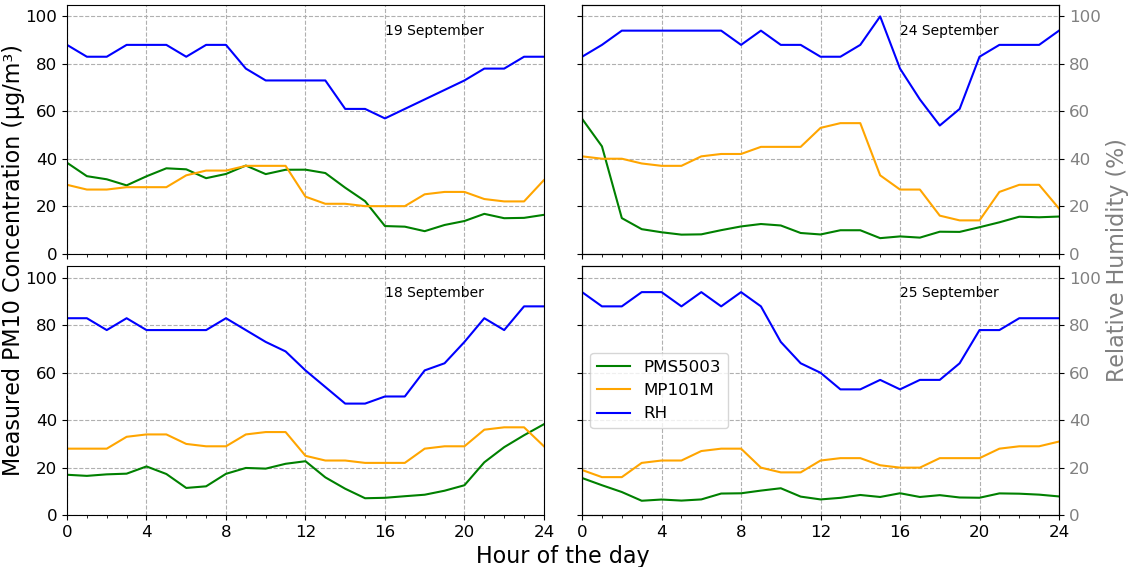
\includegraphics[width=1\textwidth]{./Images/Results/worst-and-best.png}
\caption{Measures of the days with the highest and lowest absolute errors and Pearson coefficients.}
\label{fig:worst-and-best}
\end{figure}

\pagebreak
%
% #############################################################################
\section{SIMs Testing}

In this section, SIM parametrization and performance results are presented. In the parametrization phase, the main objective is to define the best parameters for every interpolation algorithm, with main focus on FBN, which is the less documented algorithm. In both phases, error statistics are calculated in order to define whether there is an algorithm which performance stands out from the remaining.

%%%%%%%%%%%%%%%%%%%%%%%%%%%%%%%%%%%%%%%%%%%%%%%%%%%%%%%%%%%%%%%%%%%%%%%%
%               Parametrization Results
%%%%%%%%%%%%%%%%%%%%%%%%%%%%%%%%%%%%%%%%%%%%%%%%%%%%%%%%%%%%%%%%%%%%%%%%
\subsection{SIM Parametrization}

The used algorithms which have user defined parameters are IDW, OK and FBNs. In this section these parameters are tested in what regards error statistics in the 5 year dataset.

In IDW, the only user defined parameter is the power function. Through the cross validation approach application in the dataset, the power function with the best error statistics was chosen. Values of \textit{p} from 0 to 5 were tested. Results are presented in \Cref{table:idw-params}, and the value selected, which has the lowest overall MAE and RMSE values is \textit{p} = 0. 

\renewcommand\arraystretch{1.5}
\begin{table}[ht]
\centering
\caption{IDW power function comparison results.}
\label{table:idw-params}
\begin{tabular}[t]{>{\raggedright}p{0.05\linewidth}>{\centering}p{0.11\linewidth}>{\centering}p{0.11\linewidth}>{\centering}p{0.11\linewidth}>{\centering}p{0.11\linewidth}>{\centering}p{0.11\linewidth}>{\centering}p{0.11\linewidth}>{\centering}p{0.11\linewidth}>{\centering\arraybackslash}p{0.11\linewidth}}
\toprule
\multirow{2}{*}{\textit{p}}&\multicolumn{2}{c}{ENC}&\multicolumn{2}{c}{ODI}&\multicolumn{2}{c}{REB}&\multicolumn{2}{c}{SCB}\\
\cline{2-9}
&MAE&RMSE&MAE&RMSE&MAE&RMSE&MAE&RMSE\\
\midrule
0&4.57&6.34&4.97&6.59&5.79&7.37&11.15&14.88\\
1&4.74&6.25&4.97&6.62&7.19&9.04&10.73&14.34\\
2&5.69&7.38&5.15&6.88&9.40&11.94&11.06&14.64\\
3&6.80&8.79&5.61&7.52&11.11&14.33&11.80&15.42\\
4&7.76&10.06&6.17&8.26&11.92&15.49&12.47&16.15\\
5&8.54&11.09&6.60&8.86&12.24&15.94&12.90&16.62\\
\bottomrule
\end{tabular}
\end{table}

The same approach was applied in the parameter assessment of the remaining algorithms.

In OK, the variogram is the main user defined parameter. As stated in Section 3.2.2, the dataset used in this work's problem has a very low number of data points, which are sparsely located in space. This problem makes it not viable to define a custom variogram for the OK interpolation. Therefore, several pre-defined variograms were tested, in order to identify which was the most suitable for this specific interpolation problem. 

The obtained results are presented in \Cref{table:kriging-params}. The variogram model which has the lowest overall MAE and RMSE values is the linear model. 

\renewcommand\arraystretch{1.5}
\begin{table}[ht]
\centering
\caption{OK variogram comparison results.}
\label{table:kriging-params}
\begin{tabular}[t]{>{\raggedright}p{0.12\linewidth}>{\centering}p{0.1\linewidth}>{\centering}p{0.1\linewidth}>{\centering}p{0.1\linewidth}>{\centering}p{0.1\linewidth}>{\centering}p{0.1\linewidth}>{\centering}p{0.1\linewidth}>{\centering}p{0.1\linewidth}>{\centering\arraybackslash}p{0.1\linewidth}}
\toprule
\multirow{2}{*}{Variogram}&\multicolumn{2}{c}{ENC}&\multicolumn{2}{c}{ODI}&\multicolumn{2}{c}{REB}&\multicolumn{2}{c}{SCB}\\
\cline{2-9}
&MAE&RMSE&MAE&RMSE&MAE&RMSE&MAE&RMSE\\
\midrule
Linear&4.95&6.68&5.03&6.69&5.88&7.52&10.89&14.51\\
Gaussian&5.96&8.02&5.38&7.29&8.93&12.23&11.21&14.69\\
Exponential&5.42&7.24&5.14&6.87&7.28&9.38&10.94&14.49\\
Spherical&5.72&7.66&5.25&7.04&8.24&10.77&11.19&14.69\\
Power&4.97&6.68&5.08&6.77&6.12&7.89&10.88&14.49\\
Hole-effect&4.77&6.62&5.03&6.65&5.95&7.57&11.36&15.08\\
\bottomrule
\end{tabular}
\end{table}

In what regards FBN interpolation, an higher number of parameters need to be addressed, namely both testing and training epochs, the network size, the number of samples made by each neuron and the granularity of the memories of each consequent neuron.

Tests were made with several samples, with 2000 iterations, from the dataset, with the objective to assess the set of training and testing epochs, and the set of the net size, number of samples and granularity, independently, as can be observed in \Cref{table:fbn-parametrization}.

\renewcommand\arraystretch{1.5}
\begin{table}[ht]
\centering
\caption{FBN Parametrization assessment results.}
\label{table:fbn-parametrization}
\begin{tabular}[t]{>{\centering}p{0.1\linewidth}>{\centering}p{0.1\linewidth}>{\centering}p{0.1\linewidth}>{\centering}p{0.1\linewidth}>{\centering}p{0.1\linewidth}>{\centering}p{0.175\linewidth}>{\centering\arraybackslash}p{0.175\linewidth}}
\toprule
Training Epochs&Testing Epochs&Net Size&Samples&Granularity&RMSE (μg/m³)&MAE (μg/m³)\\
\midrule
%TODO:
10&10&15&4&2&13.99&18.35\\
50&50&15&4&2&13.63&17.96\\
\midrule
%TODO:
10&10&75&9&3&11.22&14.80\\
50&50&75&9&3&10.98&14.54\\
\midrule
%TODO:
10&10&125&16&4&12.94&16.91\\
50&50&125&16&4&12.05&15.92\\
\bottomrule
\end{tabular}
\end{table}

From further studying and experimenting with FBNs, it was observed that:

\begin{itemize}
    \item Performance increased with the number of testing and training epochs;
    \item Similarly to the observed in other studies \cite{Tome2014}, the number of samples should be substantially lower than the net size;
    \item When very low granularity values are used, consequent neurons will have very small memory tables. Therefore, the information sampled in sampling phases, in both learning and testing epochs, will have insufficient resolution;
    \item For high granularity values, the number of testing and learning epochs needs to be higher, than with values close to the square root of number of samples.
    \item As also pointed in previous studies, FBNs advantages lie in their ability to obtain very good results without extensive parameterization efforts \cite{Tome2014}.
\end{itemize}

% Discussion - FBNs
%The following statements can be concluded from these %results:
%\begin{itemize}
%    \item Testing and training epochs do not have %influence in the results;
%    \item Net size, along with the number of samples %and granularity increase leads to consistently %better results, in terms of both \ac{MAE} and %\ac{RMSE}.
%\end{itemize}

% Discussion - FBNs
% A substantial increase in computing times with the increase of the network size was observed. If larger network sizes would be used, with large datasets, execution times would increase to impractical values.

The chosen parameters for the FBN interpolation, accounting the previous results, are presented in \Cref{table:fbn-chosen-parameters}.

\renewcommand\arraystretch{1.5}
\begin{table}[ht]
\centering
\caption{Choice of parameters for FBNs used in this work.}
\label{table:fbn-chosen-parameters}
\begin{tabular}[t]{>{\centering}p{0.17\linewidth}>{\centering}p{0.17\linewidth}>{\centering}p{0.17\linewidth}>{\centering}p{0.17\linewidth}>{\centering\arraybackslash}p{0.17\linewidth}}
\toprule
Training Epochs&Testing Epochs&Net Size&Samples&Granularity\\
\midrule
50&50&75&9&3\\
\bottomrule
\end{tabular}
\end{table}

FBN interpolation performance was also tested using the dataset with measures corresponding to 15 minute intervals, as referred in Section 3.2.3. This test main objective is to analyze how resolution of data influences FBNs interpolation performance.

The resulting error statistics are presented in \Cref{table:fbn-15mins}.

\renewcommand\arraystretch{1.5}
\begin{table}[ht]
\centering
\caption{FBN 15 minute improvements.}
\label{table:fbn-15mins}
\begin{tabular}[t]{l>{\centering}p{0.08\linewidth}>{\centering}p{0.08\linewidth}>{\centering}p{0.08\linewidth}>{\centering}p{0.08\linewidth}>{\centering}p{0.08\linewidth}>{\centering}p{0.08\linewidth}>{\centering}p{0.08\linewidth}>{\centering}p{0.08\linewidth}>{\centering}p{0.08\linewidth}>{\centering\arraybackslash}p{0.08\linewidth}}
\toprule
&\multicolumn{2}{c}{AVL}&\multicolumn{2}{c}{ENC}&\multicolumn{2}{c}{OLI}&\multicolumn{2}{c}{RES}&\multicolumn{2}{c}{SCB}\\
\midrule
{} &MAE&RMSE&MAE&RMSE&MAE&RMSE&MAE&RMSE&MAE&RMSE\\
\midrule
Regular FBN      & 8.36 & 10.99 & 7.18 & 9.52  & 9.72  & 11.97 & 6.05 & 9.38  & 6.53 & 9.68\\
15min FBN        & 9.42 & 12.49 & 8.87 & 11.87 & 10.77 & 13.35 & 6.72 & 10.41 & 6.50 & 10.17\\

\bottomrule
\end{tabular}
\end{table}

% TODO: alterar estes valores quando atualizar a tabela
In the regular FBN execution these values were 7.57 and 10.57, which are better than the 15 minute implementation, which were 8.46 and 11.71. 


% Discussion - FBNs
%Worse performance was observed in the FBN execution with the 15 minute interval resolution, which leads to the conclusion that the number of training rules used for each interpolation has no influence on the overall inference performance of FBNs.

%
%%%%%%%%%%%%%%%%%%%%%%%%%%%%%%%%%%%%%%%%%%%%%%%%%%%%%%%%%%%%%%%%%%%%%%%%
%               SIM comparison results and analysis
%%%%%%%%%%%%%%%%%%%%%%%%%%%%%%%%%%%%%%%%%%%%%%%%%%%%%%%%%%%%%%%%%%%%%%%%

\subsection{SIM Comparison}

Every algorithm considered so far in this work was tested with the cross validation approach in the 5 year dataset. 
%Other simpler interpolation algorithms, with no user defined parameters, were additionally added to the tests, namely the Linear Interpolation and the Nearest Neighbors interpolation algorithms.

Results regarding the error statistical parameters MAE and RMSE of every algorithm are presented in table \Cref{table:sim-comparison}, for a total of 43 956 single inferences each.

\renewcommand\arraystretch{1.5}
\begin{table}[ht]
\centering
\caption{Model comparison results.}
\label{table:sim-comparison}
\begin{tabular}[t]{l>{\centering}p{0.1\linewidth}>{\centering}p{0.1\linewidth}>{\centering}p{0.1\linewidth}>{\centering}p{0.1\linewidth}>{\centering}p{0.1\linewidth}>{\centering}p{0.1\linewidth}>{\centering}p{0.1\linewidth}>{\centering\arraybackslash}p{0.1\linewidth}}
\toprule
&\multicolumn{2}{c}{ENC}&\multicolumn{2}{c}{ODI}&\multicolumn{2}{c}{REB}&\multicolumn{2}{c}{SCB}\\
\midrule
{} &MAE&RMSE&MAE&RMSE&MAE&RMSE&MAE&RMSE\\
\midrule
IDW&4.65&6.52&4.89&6.48&5.46&6.97&11.52&15.31\\
OK&4.67&6.52&4.89&6.49&5.55&7.06&11.41&15.18\\
FBN&5.82&7.62&6.36&8.41&7.55&9.62&11.08&14.75\\
Linear&5.90&7.74&6.59&9.46&10.11&13.11&11.04&14.51\\
NearestN&11.20&14.63&7.35&9.82&12.58&16.36&13.45&17.22\\
\bottomrule
\end{tabular}
\end{table}


The algorithms with the overall lower MAE and RMSE results were IDW, with 6.42 μg/m³ and 9.25 μg/m³, respectively, and OK, with 6.42 μg/m³ and 9.23 μg/m³. NN with 11.03 μg/m³ and 14.66 μg/m³, had the worse results, followed by LI, with 8.28 μg/m³ and 11.36 μg/m³. FBN results were 7.55 μg/m³ and 10.24 μg/m³. Density scatter diagrams and histograms of the IDW, OK and FBN algorithms can be observed in \Cref{fig:performance-scatter-diagrams} and \Cref{fig:performance-histograms}. % TODO


% TODO Mudar para os anexos.
\begin{figure}[ht]
\centering
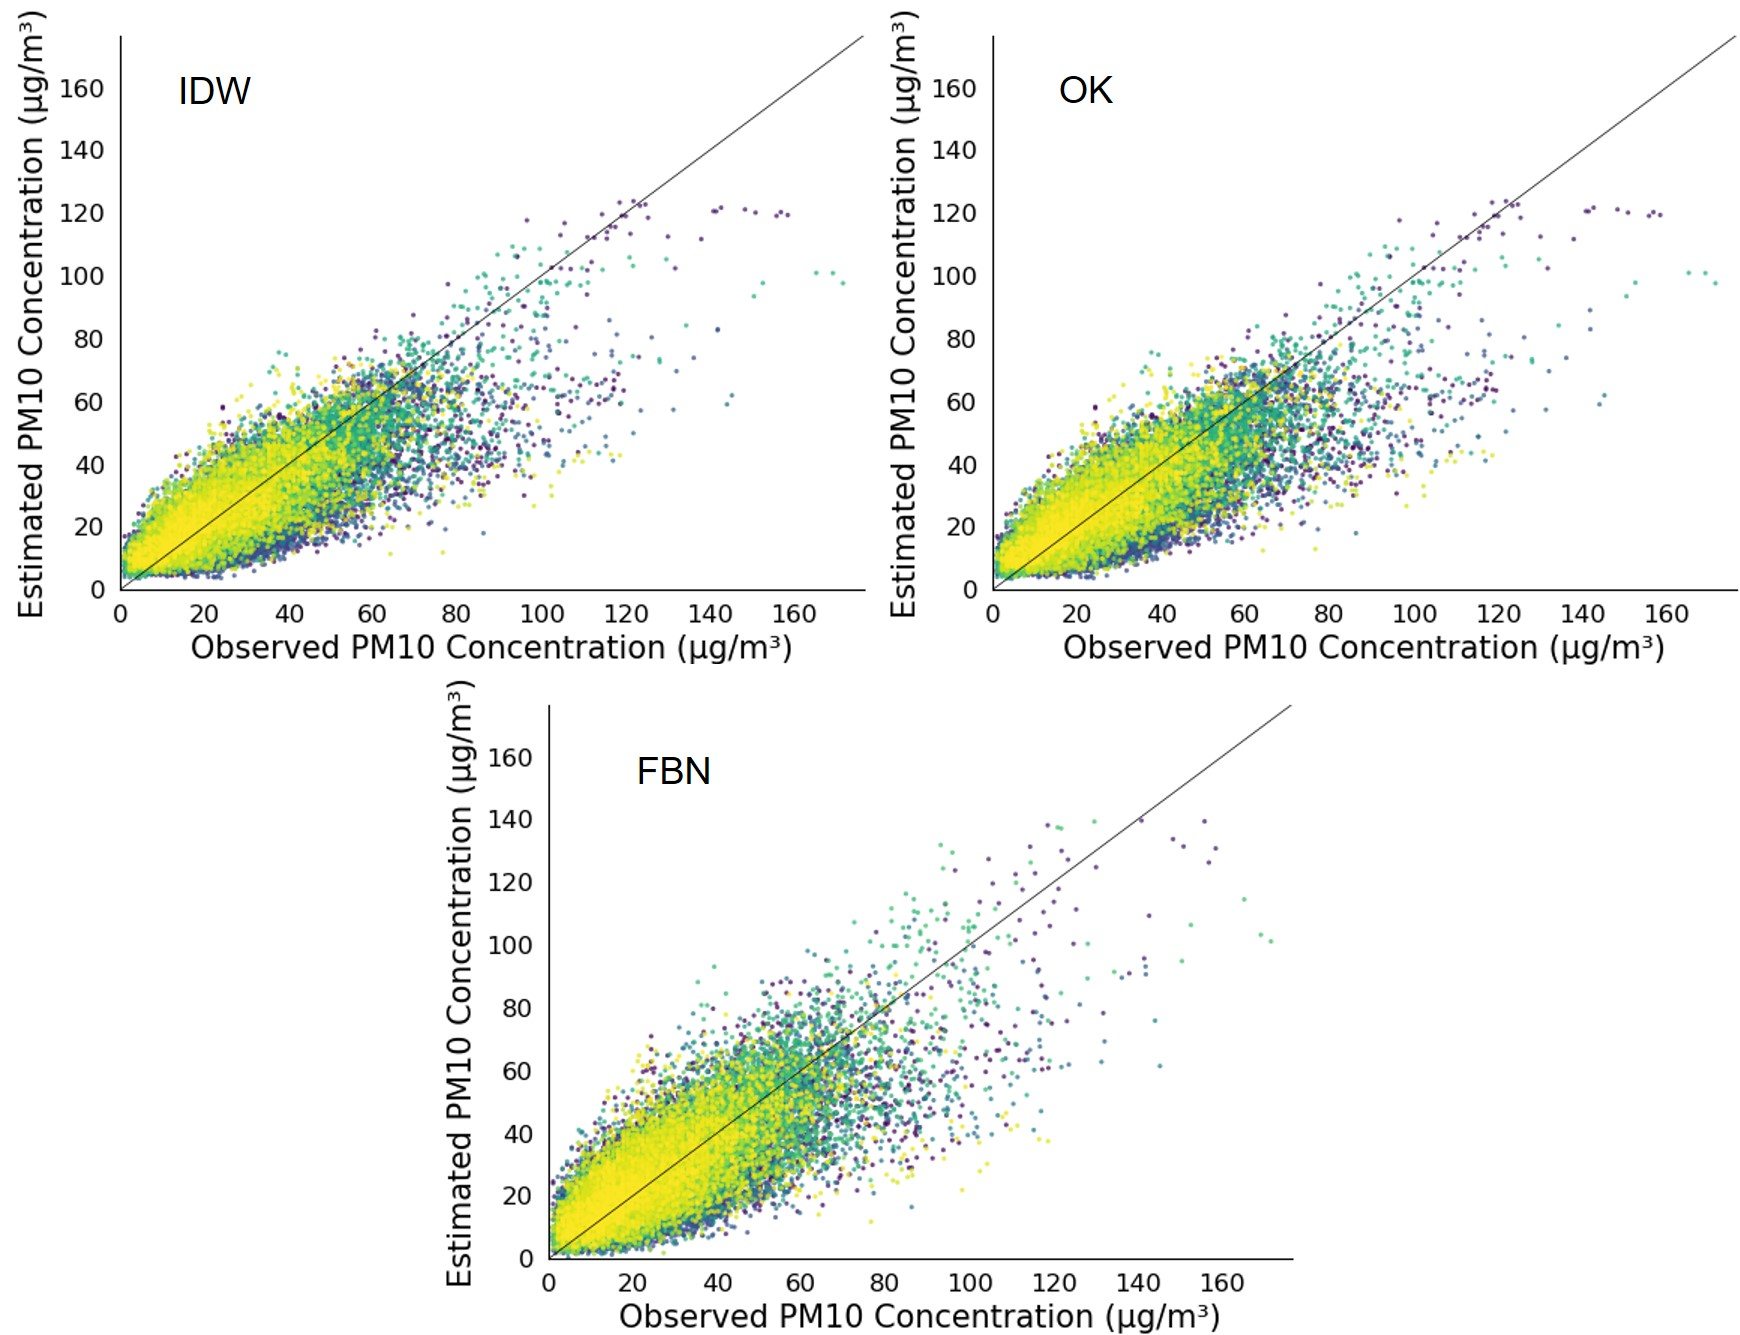
\includegraphics[width=0.8\textwidth]{./Images/Results/performance-scatter-diagrams.jpg}
\caption{Scatter diagrams obtained from 43 956 inferences for IDW, OK and FBN, respectively.}
\label{fig:performance-scatter-diagrams}
\end{figure}

It should additionally be noted that FBNs execution times of the obtained results took approximately 9 hours, while every remaining algorithm only took from 5 to 10 minutes interpolating through the entire dataset.

% Discussion - FBNs
%This again adds to the conclusion that FBNs have less practical application in large dataset problems.

% Discussion - Algorithms
%It is important to note that despite worse values RMSE and MAE for the FBNs, these still represent error values which are under variations of 14 μg/m³, which corresponds to the smallest classification interval of the \ac{PM10} concentration values official classification.

\begin{figure}[ht]
\centering
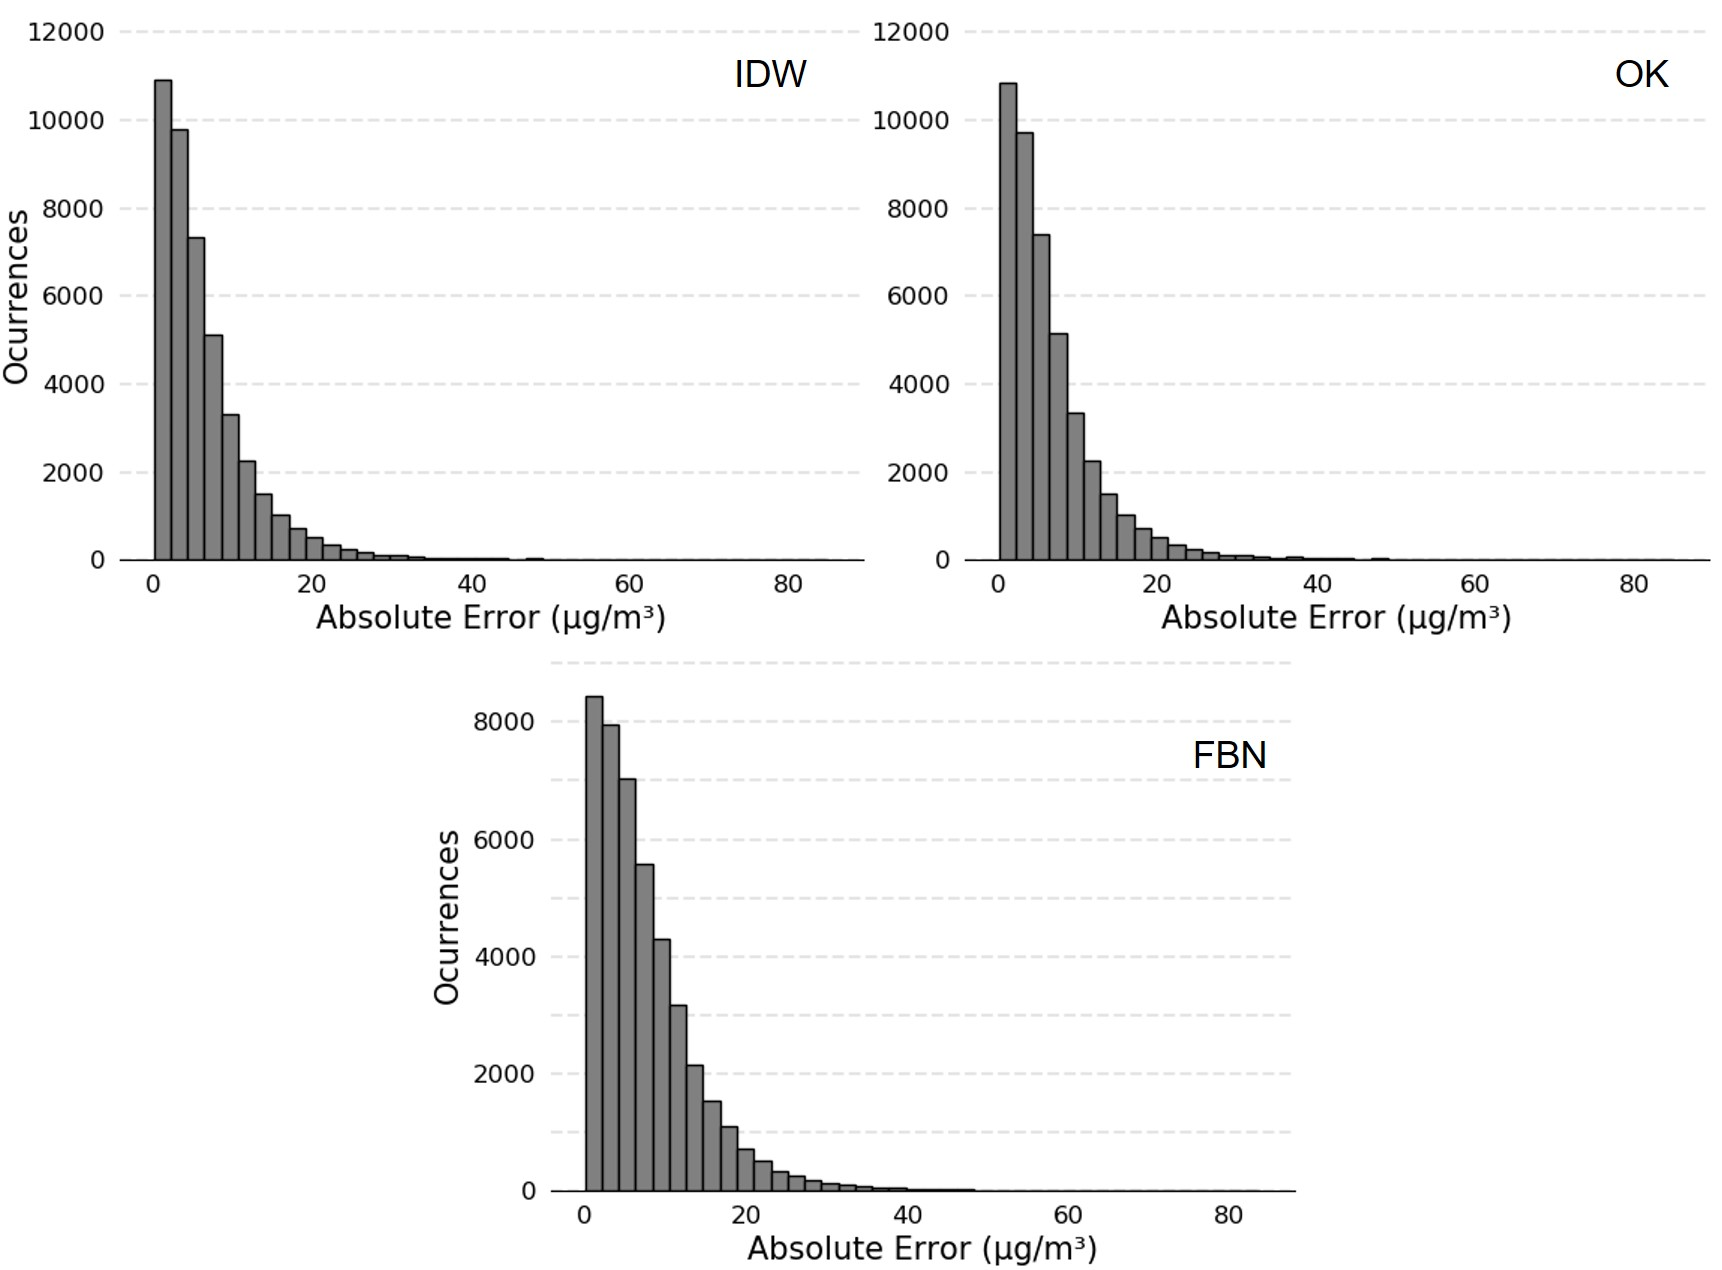
\includegraphics[width=0.8\textwidth]{./Images/Results/performance-histograms.jpg}
\caption{Histograms obtained from 43 956 inferences for IDW, OK and FBN, respectively.}
\label{fig:performance-histograms}
\end{figure}

% Para introduzir aqui secção sobre as FBNS:
%- mencionar em: 
%   - introducao capitulo 4, discussao, e conclusao.

%
% É concluído que nao ha correlação espacial suficiente para que sejam retiradas conclusoes relativamente ao desempenho das FBNs em interpolação espacial.
% Esta secção terá uma ou duas experiencias com dados estocasticos simulados e de alta correlação espacial, num plano, para fazer inteprolação 2d com as fbns e testar a sua performance contra outros algoritmos num ds com alta spatial autocorrelation.

\section{Online Data Visualization Web Application}

The developed PM10 visualization application was created to present a tool to visualize tested geographical interpolation algorithms and also to constitute a prototype for a platform of live online visualization of interpolated air quality related phenomena.

The resulting prototype is an application with PM10 interpolated data for the city of Lisbon. It has a resolution of 100 meters, both in color and in height of the pollution surface. It provides the possibility to hover over to know estimated PM10 concentration values in any location inside the outline defined by the CCDR-LVT monitoring network stations.

The application design is focused in the user experience, and allows the user to zoom in and out, and change both pitch and bearing of the map.

The final result of the developed web application is presented in \Cref{fig:developed-visualization} and is available at \url{http://138.68.165.208/}.

% Alterar esta figura para uma mais atualizada
\begin{figure}[ht]
\centering
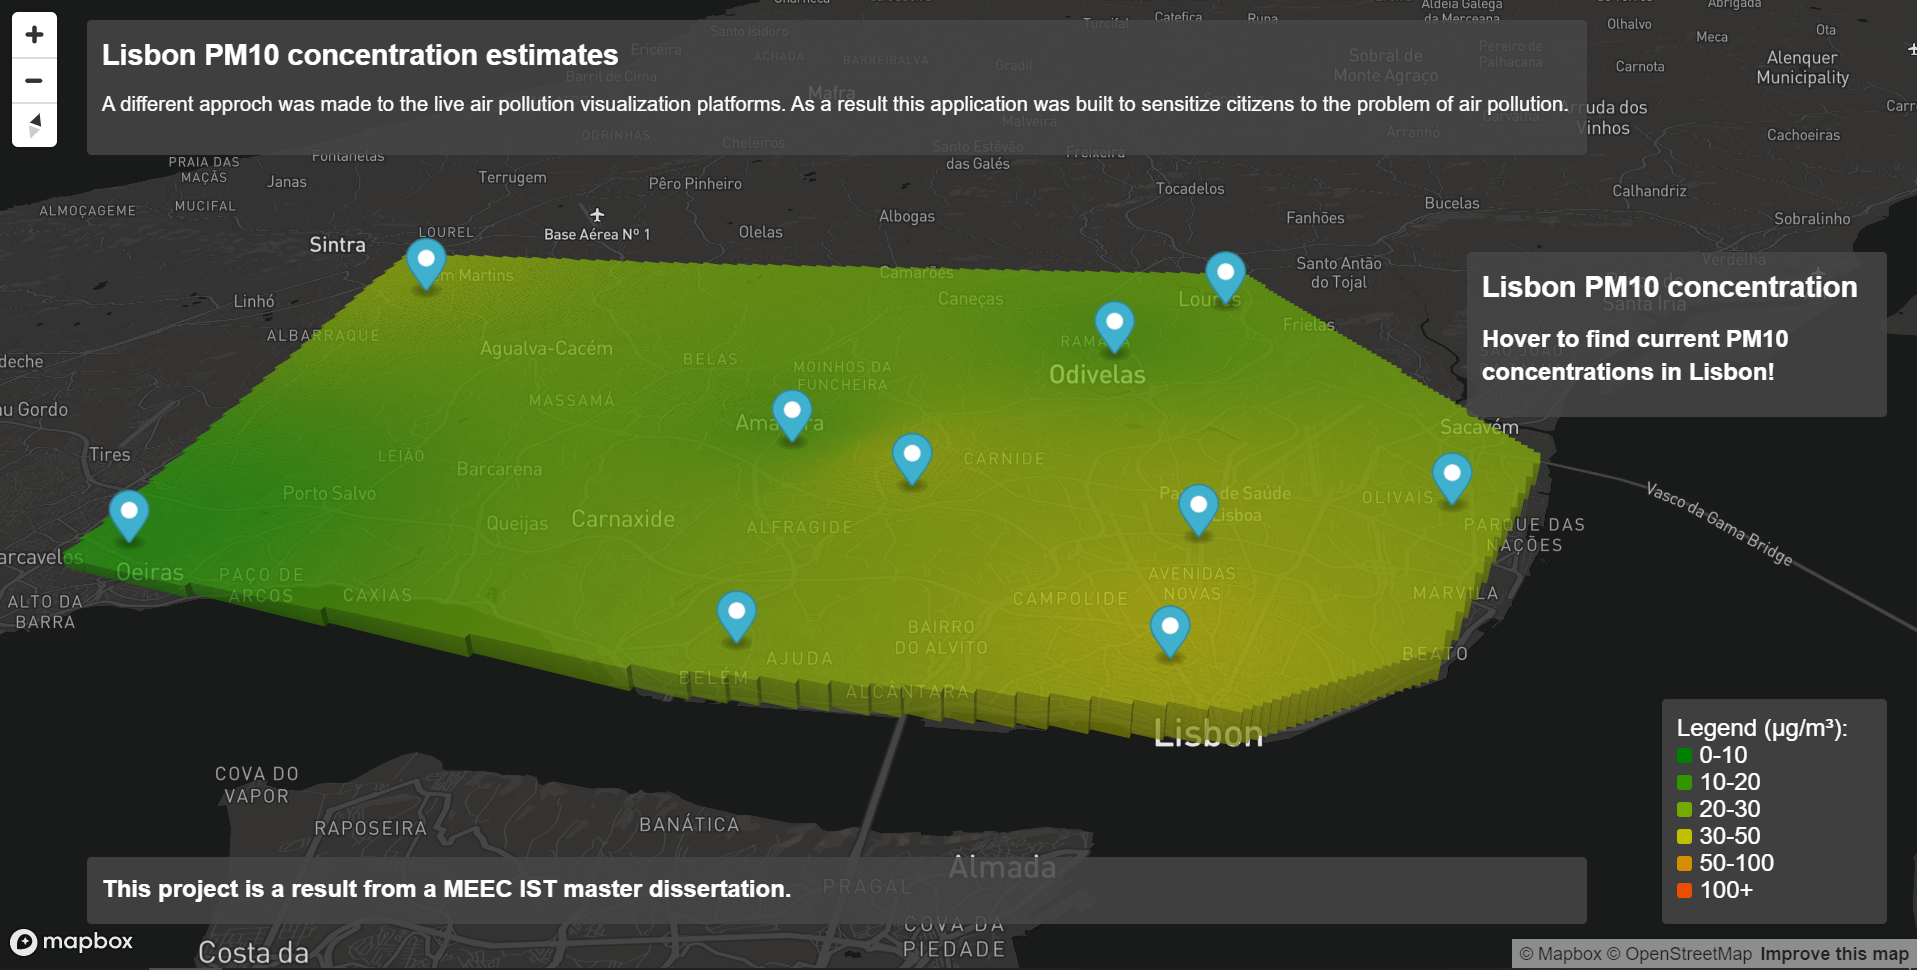
\includegraphics[width=1\textwidth]{./Images/Results/developed-visualization.PNG}
\caption{Developed web application final result, with live data from QualAr, interpolated with OK.}
\label{fig:developed-visualization}
\end{figure}

In \Cref{table:access-times} are presented the access times of some of the platforms for air pollution visualization referenced in this work, on comparison to the developed one. These results were provided from tests from Pingdom tool for web page performance assessment \cite{pingdom}.

\begin{table}[ht]
\centering
\caption{Access times of various air quality visualization web pages.}
\label{table:access-times}
\begin{tabular}[t]{l>{\centering}p{0.18\linewidth}>{\centering}p{0.13\linewidth}>{\centering\arraybackslash}p{0.16\linewidth}}
\toprule
Web Page&Access Time (ms)&Requests&Page Size (MB)\\
\midrule
138.68.165.208 (developed application)&207&44&7.5\\
airindex.eea.europa.eu&2580&77&3.8\\
qualar.apambiente.pt&3400&180&9.1\\
breezometer.com/air-quality-map/city/lisbon&3629&184&2.2\\
\bottomrule
\end{tabular}
\end{table}

% Se houver tempo, optimizar o ficheiro geojson https://docs.mapbox.com/help/troubleshooting/working-with-large-geojson-data/
% e colocar aqui uma tabela com tempos de acesso a alguns websites



\section{Discussion}

Results obtained and presented in this chapter are discussed in this section.

\subsection{Developed PM10 Monitoring System}

%%
Regarding the NB-IoT coverage in Portugal, from both MEO and NOS, namely in the capital Lisbon, it could be concluded that it is not good enough for professional applications at the time of this work.
During the 10 weeks of placement of the developed system, in different locations in the city of Lisbon, there were only 2 weeks when it was possible to get consistent coverage.

According to its specifications, overviewed in Section 2.4.4, NB-IoT has one of the widest coverages between IoT technologies. This was not observed in this work. It might have happened because NB-IoT is still in early implementation stages in Portugal.

These results demonstrate that the developed sensor, at the time of this work, from the network coverage perspective, can not be employed neither integrate current official monitoring networks.

Before assessing the used low-cost sensor performance, it is important to note that the obtained data only corresponds to a period of approximately two weeks as presented in \Cref{table:measurement-period}, which represents a small sample size in comparison to what was expected, due to the NB-IoT network coverage constraints.


% observations

During the sensor placement and comparison period, the PMS5003 sensor often obtained lower measures. However, sometimes it peaked, surpassing the MP101M measures. This only happened for high values of RH. It additionally can be observed in \Cref{fig:system-calibration} that when the RH is decreasing is when often less error is observed between the sensors.

% error statistics
The average absolute error between the measures of the different sensors (14.40 μg/m³) is slightly above the smallest scale division in \Cref{table:pm10-classification}. In the scatter diagram of \Cref{fig:scatter-measurements} it can be observed that the developed system measured values are predominantly lower than the reference measures. The daily pearson correlation coefficients (\Cref{table:pearson-coefs-sensor}) showed inconsistency in the linearity between sensor readings.

%temperature
PMS5003 sensor manufacturers claim that the sensor presents high consistency in the temperatures between 10 and 40ºC \cite{Sayahi2018}. It was summer season during this experiment, and the temperature values never exceeded positively nor negatively the above mentioned interval. 
However, the reference monitor has a controlled sampling flow rate of 1 m³/h, as well as a temperature-regulated sampling tube. This does not happen in the PMS5003, in which neither air flow nor its temperature are controlled.
Furthermore, it is important to note that the low-cost sensor was placed in the outside of the monitoring container, while the reference monitor was placed on the inside.

% rain
The only rain occurrences during the placement periods happened in the day 21 of September. It is the day with the second highest absolute error between readings, and PMS5003 measures were very low in comparison to the MP101M.

% humidity
In a study by Zheng et al., in 2018, a similar sensor model (PMS3003) was extensively tested against professional reference monitors and it was observed that while temperature took a negligible part in the difference observed between sensors, RH had a considerable influence in the deviation observed in the low-cost sensor \cite{Zheng2018}. This can be the one cause for the high observed error and linearity inconsistencies in this work experiment.

Humidity can have a negative effect on electronic circuits, such as the one in the developed system. However, no recurrent effects were observed due to humidity peaks specifically in the PMS5003 readings.

The registered high humidity intervals correspond to night and dawn periods. Similar to what happened in a study by Jayaratne et al., in 2018, in these periods, measures are often higher than in the rest of the time. The increase of measured values when there is high humidity is expected in the PMS5003 due to its documented humidity sensitivity, however it suggests that the MP101M is also influenced by high RH.

In the same study, it was stated that above 75\% humidity, marked effects are seen in low-cost sensors due to air particle size growth by deliquescence, specially if these do not have drying facilities at the sample inlets \cite{Jayaratne2018}. However, in this work, no effect in the PMS5003 was observed in high humidity periods. There is a substantial increase in measured values, but coincident with the increase reported by the MP101M, and there are undervalued measurements during the rain periods.

% car traffic
The days 14, 15, 21 and 22 of September corresponded to weekend days, which often means there is less car traffic in AVL. No meaningful tendencies were observed in these days, despite the average PM10 concentration being slightly lower in both sensors.

During the day, MP101M readings are mostly higher than PMS5003's.
According to Jayaratne et al., in the same study \cite{Jayaratne2018}, this may happen because the size of traffic particles are below the minimum detectable size limit of low-cost sensors, which for the PMS5003 is 0.3 µm (300 nm). As presented in a study by Li et al., in 2018, where the size-resolved mass concentration of volatile and non-volatile components of vehicle emitted particles is studied, the diameter of particles emitted by vehicles was mostly below 300 nm, which corroborates the fact these are not accordingly measured by the PMS5003 \cite{Li2018}.

% conclusion on placement in official networks
The objective of this experiment was to find out whether it is possible to define a correction factor for the low-cost sensors, through which they could provide PM10 readings with very low error in comparison with reference monitors. Results show that the absolute error between sensors is not linear neither correlated with the absolute value of RH. Therefore appropriate correction factors are not possible to derive with the obtained data.

Due to the numerous disadvantages observed in this work, it can be concluded, with this work data, that low-cost sensors are not suited for regulatory applications, such as assess if the air quality meets stipulated guidelines for particle pollution. However, with previous study of the placement location, such as average particle size and overall RH, and the deduction of a fitting correction factor to that specific location, it could be used for informative purposes, for example in interpolation platforms, to provide a better resolution to monitoring networks which currently suffer from sparsity.

% Comparing conclusions to other works conclusions
In mentioned studies concerning PMS low-cost sensor calibration, it was concluded that appropriate calibration models using dynamic adjustments for meteorological parameters are an essential prerequisite for these sensors to achieve high accuracy and precision in the ambient monitoring and that after proper calibration, low-cost PM sensors can be promising monitors for PM sensor network development and to complement the existing networks, without specifying its integration in official networks \cite{Zheng2018}.


%One calibration approach which could be considered, through what is observed in \Cref{fig:scatter-measurements}, which are predominantly lower measured values in the low-cost sensor, is the simple increase of the values below 10 ug/m3 to the double of its value, which would reduce the error between measures. This could lower the error only to a certain value, however it is not considered to be good enough as a calibration function, since it only covers a small number of measures, and the special case of low pollution. It also would not allow the sensor to take accurate enough measures for it to be used as a data point for interpolations and even in terms of integration in the official monitoring networks.


\subsection{SIMs Assessment}

The algorithms with the best overall performance were IDW and OK, followed by FBNs, LI and lastly NN.

In \Cref{table:correlation-coef}, correlation coefficients between every station of the dataset was calculated. It can be observed that the stations with the highest correlation coefficients between them were relatively close in terms of geographical location, despite an overall big correlation observed between almost every station.

The high performance of IDW with \textit{p} = 0, which means that distance between data points is not considered for the calculation of the interpolated values, suggests that the distance correlation between stations is low.

%This could help formulate the hypotheses of the high spatial correlation between stations. However, the fact that an algorithm where distances between station was the one with the best performance leads to the conclusion that this hypotheses is not valid.

Air dispersion and movement in urban environments is an environmental problem of high complexity, due to its influence by many factors. In the last 5 years, in the city of Lisbon, the dataset reveals the city to have an overall low concentration of PM10, with maximum mean value for the whole dataset, between every station, being 34.22 ug/m3 in the station AVL, which is a value classified as \textit{Good}.

The fact that these SIMs were tested for periods where no big pollution phenomena affected the city, could degrade the sense of distance correlation between the stations in the city, because the collected data was predominantly constant and similar between stations.

Other environmental factors can influence the correlation of air quality throughout the city, such as the wind direction, the temperature, humidity, the altitude of the interpolation point and the traffic density and pollution, as well as the presence of buildings and other geological and geographical barriers to airflow.

In what regards FBNs performance, no conclusions can be obtained towards its performance regarding multi dimensional spatial interpolation problems due to the low distance correlation between the data points of the performed experiments. However it can be concluded that FBNs are not suitable for problems which require real time interpolations with fast computations and construction of interpolation surfaces, due to the long computing times observed in this work.



%%
%Contudo, pode concluir se que, no problema da qualidade do ar, provavelmente devido aos edifícios etc e outras barreiras geológicas , a simples relação espacial dos dados através de distância horizontal pode não ser indicada.

%Sugere q o problema da qualidade do ar é mt complexo e q portanto é essencial promover a interaçao entre equipas multidisciplinares de engenheiros informaticos e tecnicos ambientais no sentido de entender que fatores externos devem ser contabilizados no algoritmo de interpolaçao e melhorar a previsao espacial de dados. 
%[FALAR Q AS COISAS SAO MULTIDISCIPLINARES E MT COMPLEXAS E Q DEVE HAVER INTERAÇAO ENTRE PROFISSIONAIS DÁ SEMPRE BOM ASPETO A UMA CONCUSAO AHAHAHAH] TODOO







% Faltam conclusões sobre as FBNs

\subsection{Web Visualization Application}

The developed application resulted in a user-friendly platform, with the presentation of live PM10 concentration data with high resolution in the area covered by the CCDR-LVT monitoring stations network in Lisbon.
Since results obtained from the low-cost sensors reveal these sensors lack performance, without specific calibration corrections, these were not included in the network used for the spatial interpolation in the application.

%%
%Como os resultados obtidos pelos sensores criados não foram precisos, optou-se por não incluí-los para já na rede de estações utilizadas na previsão espacial de dados. 

%[tens q explicar porque nao usaste os sensores moveis no site, pois tinhas dito no state pf art que esta seria uma hipotese q tavas a testar ]


The application has good performance and is flexible from a development point of view. It can easily be extended to support several other air polluting gases concentration or indicators. The same structure could additionally be applied in other geographical interpolation fields.

In what concerns web page performance, the developed application has an extremely lower access time than other mentioned web pages, as well as a less number of requests. This is expected since it does not use any kind of back end processes, besides the ones of Mapbox GL JS, and is only composed of a map with interpolated data, while other web pages have several more web elements and components which can cause delays in access times. High page size was also observed and expected, since no component compression was built into the application.

In comparison with current governmental web applications available, the developed application has higher resolution and provides better user experience, despite still not covering large areas such as whole countries. Furthermore, it is already prepared for a future state of official monitoring networks with increased density of monitoring stations and an interpolation representation which accuracy is expected to rise with the increase of data points.

As a product, there are already companies with applications which outperform it, as seen in Section 2.6 of this work, being the most evident Breezometer.

Breezometer presents data regarding numerous air polluting gases and indicators with a resolution of 500 meters \cite{Breezometer}, and worldwide coverage. However, due to its proprietary characteristics, its used air modelling algorithms and used tools are not documented and consequently not available for assessment.

It is important to note that the characteristics enumerated do not constitute disadvantages of the developed application, but rather a comparison and position of the developed prototype with the state of the art of the current web visualization applications for air quality pollution.

It can be concluded that the developed platform could bring awareness to the citizens in what regards their cities air quality, in high resolution, and constitute a replacement for current government platforms.
% If Printing on DOUBLE SIDED pages, the second page should be white.
% Otherwise, comment the following command:
\cleardoublepage
%
%Chapter 5
% #############################################################################
% This is Chapter 5
% !TEX root = ../main.tex
% #############################################################################
% Change the Name of the Chapter i the following line
\fancychapter{Conclusion}
\cleardoublepage
% The following line allows to ref this chapter
\label{chap:conclusion}

The main objective of the work developed in this master thesis is the analysis of the current state of the information available publicly regarding air quality, namely PM10 concentration data, in the city of Lisbon, and to experiment with different technologies which could improve it. This was done through the development of a prototype for a low-cost PM10 sensor node with the use of the NB-IoT technology, the creation of a live PM10 concentration visualization application, and the assessment of various spatial interpolation algorithms in the inference of PM10 concentration in the city of Lisbon, with the limited data points available of the CCDR-LVT air quality monitoring network.
This work conclusions solidify knowledge on the application of every used technology, in the field of air quality monitoring, interpolation and visualization.

% #############################################################################
\section{Conclusion}

The developed low-cost sensor was successfully deployed in AVL station for two weeks. Measures were taken and compared with the simultaneous reference AVL PM10 monitor. Results showed an error of 14.40 μg/m³ between the two, which is slightly above the smallest scale division of PM10 classification. Inconsistent linearity was observed during the whole period, through the calculated daily Pearson correlation coefficients. Finally, it was concluded that the sensor is not able to integrate current official monitoring networks, and further experiments should be made to better understand these low-cost sensors calibration adjustments.

The spatial interpolation algorithms tested, with data constituting 5 years of Lisbon's monitoring network measurements, from 2013 to 2017, revealed that there is not an high distance correlation between the stations in the network, in terms of geographical location influence. These were used only with geographic coordinates, and pollution in Lisbon was considered low in the considered 5 years, with very sparse data points, specially accounting the present urban topology, which might constitute reasons for why IDW with \textit{p} = 0, was one of the best performing algorithms. Finally, the developed online visualization platform resulted in a web application which can provide PM10 data with finer resolution than other current available platforms, even though it only covers the city of Lisbon, and in an approach which can be used by further studies and platforms to represent geographical interpolation phenomenons online.

As an overall conclusion to this work, the current state of the data available publicly regarding air quality was studied and assessed and several experiments were made in other to evaluate the application of new technologies, and the creation of prototypes, which could improve it. Relevant results were obtained regarding the usage and performance of every technology used and applied in this work. Finally, information was gathered for further study of the phenomenon of spatial interpolation of air quality, its measurement and its visualization.

%Several other variables should be measured at the placement location, in order to conclude on how susceptible that low-cost sensor is to different environment conditions. However, the used board, SODAQ SFF R412M did not work appropriately with both PMS5003 and any of the available sensors tested (DHT11, DHT22 and BME280), simultaneously.


\section{Future Work}

% NB-IoT + Sensor
In a study using NB-IoT, several tests and an evaluation of the study area coverage should be made previously to its application. These tests should be made in the field and with several different mobile operators and different NB-IoT chipsets, in order to deduce coverage constraints and hardware limitations.

Low-cost PM monitoring sensors, should be studied beforehand in controlled environments. Various tests should be made with different conditions in order to evaluate the deviations between measures as an answer to real world conditions.

Ideally, with a very well understanding of this sensor properties, and a calibration function which could minimize the error to extremely low values, for each specific placement location, this type of sensors could integrate air quality monitoring networks, but only to further increase their spatial density and the resolution at which air quality could be visualized. This would ultimately improve researchers understanding of air quality phenomenons, and propel research progress in related fields of study.

%Spatial Interpolation Models
Spatial algorithms tested in this work could be studied and complemented with air dispersion models. Data could be gathered for certain long periods of time for variables such as traffic, wind direction, temperature, altitude and relative humidity, and could be incorporated into machine learning algorithms.

Regarding FBNs, its implementation could be parallelized, which could drastically optimize its performance, due to the parallel nature of its neuron sampling operations. It could be further studied regarding spatial geographical interpolation, with the integration of additional variables to the problem.

% WEB VIS APP
The web visualization tool developed in this work, as already pointed out in Section 4.3 of this work, could be used in the future as a visualization tool in different geographical fields. It could also be extended in order to include other air quality pollution gases and indicators.

The developed prototype could also be extended into a web application, since it is constituted predominantly by web components, through the development of an adequate application programming interface, and the deployment with a mobile app development technology, such as Ionic, which allows the development of mobile applications using web technologies such as CSS and HTML. 

% #############################################################################

% If Printing on DOUBLE SIDED pages, the second page should be white.
% Otherwise, comment the following command:
\cleardoublepage
%
% -----------------------------------------------------------------------------
% BIBLIOGRAPHY
% Add the Bibliography to the PDF table of contents (not the document table of contents)

\pdfbookmark[0]{Bibliography}{bib}
% The bibliography style sheet
% Chose your preferences on the format of the entries and the Labels:
% IEEEtran: Used in general (recommended for IST Thesis)
%           Entries are labelled and sorted by appearance in the document
%           Labels are Numeric inside square brackets
\bibliographystyle{IEEEtran}
%
% Apalike:  Entries formatted alphabetically, last name first, with identation
%           Labels with Autor's Name and Year inside square brackets
%\bibliographystyle{apalike}
%
% Alpha:    Entries formatted with Autor's Name and Year, hanging identation
%           Labels with Autor's abbr. Names and Year inside square brackets
%\bibliographystyle{alpha}
%
% Acm:     Entries formatted with Autor's Name (small Caps), hanging identation
%          Labels are Numeric inside square brackets
%\bibliographystyle{acm}
% The following command resets the 'emphasis' style for bibliography entries
\normalem
% Name of your BiBTeX file
\bibliography{./Thesis-MSc-Bibliography} % Put here your own filename
%
% The following command modifies the 'emphasis' style for bibliography entries
\ULforem
% If Printing on DOUBLE SIDED pages, the second page should be white.
% Otherwise, comment the following command:
\cleardoublepage
%
% -----------------------------------------------------------------------------
% HERE GO THE APPENDIXES IF REQUIRED
% If not required just comment the blocks
%\appendix
%% First Appendix
%\pdfbookmark[1]{Appendix A}{appendix}
%% #############################################################################
% This is Appendix A
% !TEX root = ../main.tex
% #############################################################################
\chapter{Code of Project}
\label{chapter:appendixA}

Nulla dui purus, eleifend vel, consequat non, dictum porta, nulla. Duis ante mi, laoreet ut, commodo eleifend, cursus nec, lorem. Aenean eu est. Etiam imperdiet turpis. Praesent nec augue. Curabitur ligula quam, rutrum id, tempor sed, consequat ac, dui. Vestibulum accumsan eros nec magna. Vestibulum vitae dui. Vestibulum nec ligula et lorem consequat ullamcorper. 

%% If Printing on DOUBLE SIDED pages, the second page should be white.
%% Otherwise, comment the following command:
%\cleardoublepage
%% Second Appendix
%\pdfbookmark[1]{Appendix B}{appendix}
%% #############################################################################
% This is Appendix B
% !TEX root = ../main.tex
% #############################################################################
\chapter{A Large Table}
\label{chapter:appendixB}

Aliquam et nisl vel ligula consectetuer suscipit. Morbi euismod enim eget neque. Donec sagittis massa. Vestibulum quis augue sit amet ipsum laoreet pretium. Nulla facilisi. Duis tincidunt, felis et luctus placerat, ipsum libero vestibulum sem, vitae elementum wisi ipsum a metus. Nulla a enim sed dui hendrerit lobortis. Donec lacinia vulputate magna. Vivamus suscipit lectus at quam. In lectus est, viverra a, ultricies ut, pulvinar vitae, tellus. Donec et lectus et sem rutrum sodales. Morbi cursus. Aliquam a odio. Sed tortor velit, convallis eget, porta interdum, convallis sed, tortor. Phasellus ac libero a lorem auctor mattis. Lorem ipsum dolor sit amet, consectetuer adipiscing elit.
%% If Printing on DOUBLE SIDED pages, the second page should be white.
%% Otherwise, comment the following command:
%\cleardoublepage

% -----------------------------------------------------------------------------
% And this is THE END of the IST Thesis Document
\end{document}